%!TEX TS-program = xelatex
\documentclass[a4paper, oneside]{report}

% ===== ระยะขอบ A4 ตามข้อกำหนด =====
% top=3.81cm, left=3.81cm, right=2.54cm, bottom=2.54cm
\usepackage[top=3.81cm, left=3.81cm, right=2.54cm, bottom=2.54cm, headheight=1cm]{geometry}

% ----- แพ็กเกจที่ใช้งาน -----
\usepackage{ragged2e}
\usepackage{enumitem}
\usepackage{tabularx,array}
\usepackage{graphicx}
\usepackage{makecell}
\usepackage{booktabs}
\usepackage{etoolbox}
\usepackage{titlesec}
\usepackage{indentfirst}
\usepackage{needspace}
\usepackage{caption}
\usepackage{adjustbox}
\usepackage{tocloft}

% ===== การตั้งค่าหัวข้อสารบัญ (สำหรับหน้าสารบัญโดยเฉพาะ) =====
% 1. กำหนดให้คำว่า "สารบัญ" อยู่กึ่งกลาง, เป็นตัวหนา, ขนาด 16pt
\renewcommand{\cfttoctitlefont}{\centering\bfseries\fontsize{16pt}{19.2pt}\selectfont}

% 2. กำหนดสิ่งที่อยู่หลังหัวข้อ "สารบัญ"
\renewcommand{\cftaftertoctitle}{%
	\par\nobreak
	\vskip-1.2em % ดึงบรรทัด "หน้า" ขึ้นไปให้ชิดกับ "สารบัญ"
	{\hfill\fontsize{16pt}{19.2pt}\selectfont หน้า\par}% จัดคำว่า "หน้า" ไปชิดขวา
	\vspace{0.5\baselineskip} % เว้นช่องว่างเล็กน้อยก่อนเริ่มรายการสารบัญ
}

% ===== ชื่อหัวเรื่องสารบัญ/สารบัญภาพ/สารบัญตาราง (ไทย) =====
\renewcommand{\contentsname}{สารบัญ}
\renewcommand{\listfigurename}{สารบัญภาพ}
\renewcommand{\listtablename}{สารบัญตาราง}

% ===== การตั้งค่าสารบัญ =====

% --- บท (Chapter) ---
\renewcommand{\cftchapfont}{\fontsize{16pt}{19.2pt}\bfseries} % ตัวหนา
\renewcommand{\cftchappagefont}{\fontsize{16pt}{19.2pt}\bfseries} % ตัวหนา
\renewcommand{\cftchapleader}{\cftdotfill{\cftdotsep}} % เส้นจุด
\setlength{\cftbeforechapskip}{1.0em} % ระยะห่างก่อนหน้า
\setlength{\cftchapnumwidth}{5em} % ความกว้างเลขบท

% --- หัวข้อ (Section) ---
\renewcommand{\cftsecfont}{\fontsize{16pt}{19.2pt}\selectfont} % ปกติ
\renewcommand{\cftsecpagefont}{\fontsize{16pt}{19.2pt}\selectfont} % ปกติ
\renewcommand{\cftsecleader}{\cftdotfill{\cftdotsep}} % เส้นจุด
\setlength{\cftbeforesecskip}{0pt} % ระยะห่างก่อนหน้า
\setlength{\cftsecindent}{2em} % เยื้องจากขอบ
\setlength{\cftsecnumwidth}{3em} % ความกว้างเลขหัวข้อ

% --- หัวข้อย่อย (Subsection) ---
\renewcommand{\cftsubsecfont}{\fontsize{16pt}{19.2pt}\selectfont} % ปกติ
\renewcommand{\cftsubsecpagefont}{\fontsize{16pt}{19.2pt}\selectfont} % ปกติ
\renewcommand{\cftsubsecleader}{\cftdotfill{\cftdotsep}} % เส้นจุด
\setlength{\cftbeforesubsecskip}{0pt} % ระยะห่างก่อนหน้า
\setlength{\cftsubsecindent}{4em} % เยื้องจากขอบ
\setlength{\cftsubsecnumwidth}{4em} % ความกว้างเลขหัวข้อย่อย

% ===== จัดเลขหน้า =====
\usepackage{fancyhdr}

\graphicspath{{/home/anming/Dropbox/ProJect/}}

% ย่อหน้าแบบไทย (เรียกใช้เป็นครั้งคราว)
\providecommand{\ThaiPara}[1]{%
	\par\begingroup
	\justifying
	\XeTeXlinebreakskip=0pt plus 1pt minus 0.5pt
	\indent #1\par
	\endgroup
}

% ----- ฟอนต์ไทย -----
\usepackage{fontspec}
\setmainfont{TH Sarabun New}[
Path=/home/anming/.local/share/fonts/THSarabun/,
UprightFont    ={THSarabunNew.ttf},
BoldFont       ={THSarabunNew Bold.ttf},
ItalicFont     ={THSarabunNew.ttf},
BoldItalicFont ={THSarabunNew Bold.ttf}
]
\XeTeXlinebreaklocale "th"
\XeTeXlinebreakskip = 0pt plus 1pt

% ===== ขนาดตัวอักษรทั้งเล่ม =====
\makeatletter
\renewcommand\normalsize{\@setfontsize\normalsize{16pt}{19.2pt}}
\normalsize
\renewcommand\small{\@setfontsize\small{13pt}{15.6pt}}
\renewcommand\footnotesize{\@setfontsize\footnotesize{13pt}{15.6pt}}
\renewcommand\scriptsize{\@setfontsize\scriptsize{13pt}{15.6pt}}
\renewcommand\tiny{\@setfontsize\tiny{13pt}{15.6pt}}
\renewcommand\large{\@setfontsize\large{18pt}{21.6pt}}
\renewcommand\Large{\@setfontsize\Large{18pt}{21.6pt}}
\renewcommand\LARGE{\@setfontsize\LARGE{18pt}{21.6pt}}
\renewcommand\huge{\@setfontsize\huge{18pt}{21.6pt}}
\renewcommand\Huge{\@setfontsize\Huge{18pt}{21.6pt}}
\makeatother

% ===== จัดหน้า =====
\setlength{\parindent}{1.5cm}
\setlength{\parskip}{0pt}
\emergencystretch=2em

% ===== ชื่อรูป/ตาราง =====
\captionsetup[table]{name=ตารางที่}
\captionsetup[figure]{name=ภาพที่}
\captionsetup[table]{justification=raggedright,singlelinecheck=false, labelfont=bf,textfont=bf}
\captionsetup[figure]{justification=centering, singlelinecheck=false, labelfont=bf, textfont=bf}
\AtBeginEnvironment{figure}{\centering}

% ===== ฟอนต์ตารางเริ่มต้น =====
\newcommand{\tablefont}{\fontsize{13pt}{15.6pt}\selectfont}
\AtBeginEnvironment{tabularx}{\tablefont\setlength{\parindent}{0pt}}

% ===== ไฮเปอร์ลิงก์ =====
\usepackage[hidelinks,unicode]{hyperref}

% ===== บรรณานุกรม: Numeric ต่อเนื่องทั้งเล่ม ตามลำดับอ้างในเนื้อหา =====
\usepackage{csquotes}
\usepackage[
backend=biber,
style=numeric-comp,
sorting=none,
sortcites=true,
doi=false, isbn=false, url=true
]{biblatex}
\addbibresource{./references.bib}

% หัวข้อ "บรรณานุกรม" ไทย: หนา 16pt กึ่งกลาง + (ไม่เพิ่มใน TOC)
\defbibheading{thai-bib}{
	\clearpage
	\centering\bfseries\fontsize{16pt}{19.2pt}\selectfont บรรณานุกรม\par
	\vspace{\baselineskip}
}
% แขวนบรรทัด (รายการยาวบรรทัดต่อไปเยื้อง 1.50 ซม.)
\setlength{\bibhang}{1.5cm}

% --- Use Case ID auto-increment ---
\newcounter{usecaseid}
\newcommand{\UseCaseID}[1][]{%
	\refstepcounter{usecaseid}%
	\textbf{Use Case ID: \theusecaseid}%
	\if\relax\detokenize{#1}\relax\else\label{#1}\fi
}

% คอลัมน์ Description แบบไม่เยื้อง + จัดกระจายไทย
\newcolumntype{D}{>{\noindent\parindent0pt\justifying\arraybackslash}X}

% ===== enumerate layout (global, same spec) =====
\makeatletter
\@ifundefined{LoneLabelSep}{\newlength{\LoneLabelSep}}{}
\@ifundefined{LoneLabelWidth}{\newlength{\LoneLabelWidth}}{}
\@ifundefined{LoneContentCol}{\newlength{\LoneContentCol}}{}
\@ifundefined{LtwoLabelSep}{\newlength{\LtwoLabelSep}}{}
\@ifundefined{LtwoLabelWidth}{\newlength{\LtwoLabelWidth}}{}
\@ifundefined{ExtraAlign}{\newlength{\ExtraAlign}}{}
\@ifundefined{LthreeLabelSep}{\newlength{\LthreeLabelSep}}{}
\@ifundefined{LthreeLabelWidth}{\newlength{\LthreeLabelWidth}}{}
\@ifundefined{NestedStep}{\newlength{\NestedStep}}{}
\makeatother

\setlength{\LoneLabelSep}{0.5em}
\settowidth{\LoneLabelWidth}{9.}
\setlength{\LoneContentCol}{\dimexpr 1.5cm + \LoneLabelWidth + \LoneLabelSep\relax}

\setlength{\LtwoLabelSep}{0.5em}
\settowidth{\LtwoLabelWidth}{9.9.}
\setlength{\ExtraAlign}{-2.8em}

\setlength{\LthreeLabelSep}{0.5em}
\settowidth{\LthreeLabelWidth}{9.9.9.}
\setlength{\NestedStep}{0pt}

% Level 1
\setlist[enumerate,1]{%
	label=\arabic*., align=left,
	leftmargin=1.5cm, labelindent=0pt,
	labelwidth=\LoneLabelWidth, labelsep=\LoneLabelSep,
	itemsep=0pt, topsep=0.5\baselineskip
}
% Level 2
\setlist[enumerate,2]{%
	label*=\arabic*., align=left,
	leftmargin=*,
	labelwidth=\LtwoLabelWidth, labelsep=\LtwoLabelSep,
	labelindent=\dimexpr \LoneContentCol + \ExtraAlign - \LtwoLabelWidth - \LtwoLabelSep\relax,
	itemsep=0pt, topsep=0pt
}
% Level 3
\setlist[enumerate,3]{%
	label*=\arabic*., align=left,
	leftmargin=*,
	labelwidth=\LthreeLabelWidth, labelsep=\LthreeLabelSep,
	labelindent=\dimexpr \LoneContentCol + \ExtraAlign + \NestedStep
	- \LthreeLabelWidth - \LthreeLabelSep\relax,
	itemsep=0pt, topsep=0pt
}

% ===== การตั้งค่าเลขหน้า =====
\pagestyle{fancy}
\fancyhf{}
\renewcommand{\headrulewidth}{0pt}
% เลขหน้าอยู่มุมบนขวา ระยะจากขอบบน 2.5 cm และขอบขวา 2.5 cm
\fancyhead[R]{\fontsize{16pt}{19.2pt}\selectfont\thepage}

\fancypagestyle{plain}{%
	\fancyhf{}%
	\renewcommand{\headrulewidth}{0pt}%
	\fancyhead[R]{\fontsize{16pt}{19.2pt}\selectfont\thepage}%
}

% กำหนดรูปแบบเลขหน้าสำหรับส่วนนำ (อักษรไทย)
\newcommand{\thaiPageNumber}[1]{%
	\ifcase#1\or ก\or ข\or ค\or ง\or จ\or ฉ\or ช\or ซ\or ฌ\or ญ\or
	\or ด\or ต\or ถ\or ท\or ธ\or น\or บ\or ป\or ผ\or ฝ\or พ\or ฟ\or ภ\or ม\or ย\or ร\or ล\or ว\or ศ\or ษ\or ส\or ห\or ฬ\or อ\or ฮ\fi
}

\begin{document}
	
	% ===== ส่วนนำ =====
	\pagestyle{empty}
	\IfFileExists{Cover.tex}{%==================== Cover.tex ====================

% ---------- ปกนอก (หน้า 1) ----------
\clearpage
\thispagestyle{empty}
\begingroup
\fontsize{16pt}{19.2pt}\selectfont % ทั้งหน้าตัวหนา 16pt ตามสเปก
\bfseries

% ส่วนต้น (ชื่อเรื่อง ชิดขอบบนของหน้ากระดาษ)
% จัดแบบ "ปิรามิดคว่ำ" อย่างหยาบโดยแบ่งบรรทัดแล้วจัดกึ่งกลาง
\noindent
\begin{minipage}[t]{\textwidth}
	\centering
	เว็บแอปพลิเคชันศูนย์รวมการจัดประกวดปลากัดไทย
\end{minipage}

% ส่วนกลาง (ชื่อผู้ทำ อยู่กึ่งกลางระหว่างท้ายชื่อเรื่องกับต้นส่วนท้าย)
\vspace*{\fill}
\begin{center}
	เอกสิทธิ์ อัศวดารา
\end{center}

% ส่วนท้าย (ข้อความบล็อกด้านล่าง)
\vspace*{\fill}
\noindent
\begin{minipage}[b]{\textwidth}
	\centering
	ภาคนิพนธ์เสนอมหาวิทยาลัยพะเยา เพื่อเป็นส่วนหนึ่งของการศึกษา\\
	หลักสูตรปริญญาตรี วิทยาศาสตรบัณฑิต\\
	สาขาวิทยาการคอมพิวเตอร์\\
	กันยายน พ.ศ. 2568\\
	ลิขสิทธิ์ของมหาวิทยาลัยพะเยา
\end{minipage}
\par
\endgroup
\clearpage

% ---------- หน้าเปล่า (หน้า 2) ----------
\thispagestyle{empty}\null\clearpage

% ---------- ปกใน (ไทย) (หน้า 3) ----------
\thispagestyle{empty}
\begingroup

\noindent
\begin{minipage}[t]{\textwidth}
	\centering
	เว็บแอปพลิเคชันศูนย์รวมการจัดประกวดปลากัดไทย
\end{minipage}

\vspace*{\fill}
\begin{center}
	เอกสิทธิ์ อัศวดารา
\end{center}

\vspace*{\fill}
\noindent
\begin{minipage}[b]{\textwidth}
	\centering
	ภาคนิพนธ์เสนอมหาวิทยาลัยพะเยา เพื่อเป็นส่วนหนึ่งของการศึกษา\\
	หลักสูตรปริญญาตรี วิทยาศาสตรบัณฑิต\\
	สาขาวิทยาการคอมพิวเตอร์\\
	กันยายน พ.ศ. 2568\\
	ลิขสิทธิ์ของมหาวิทยาลัยพะเยา
\end{minipage}

\par
\endgroup
\clearpage

% ---------- ปกใน (อังกฤษ) (หน้า 4) ----------
\thispagestyle{empty}
\begingroup


% Title (approx. translation; แก้คำแปลได้ตามที่ต้องการ)
\noindent
\begin{minipage}[t]{\textwidth}
	\centering
	Web Application for the Centralized\\
	Thai Betta Fish Competition
\end{minipage}

\vspace*{\fill}
\begin{center}
	% เปลี่ยนเป็นสะกดชื่ออังกฤษที่ต้องการได้
	Aekkasit Oatsawadara
\end{center}

\vspace*{\fill}
\noindent
\begin{minipage}[b]{\textwidth}
	\centering
	A Term Paper submitted to the University of Phayao in Partial Fulfillment of the\\
	Requirements for the bachelor’s degree. Bachelor of Science.\\
	Department of Computer Science\\
	Computer Science Program\\
	September 2025\\
	Copyright belongs to the University of Phayao
\end{minipage}

\par
\endgroup
\clearpage

%================== จบ Cover.tex ==================
}{}
	\IfFileExists{Approval.tex}{%==================== Approval.tex ====================

\clearpage
% \thispagestyle{empty}

\begingroup
\fontsize{16pt}{19.2pt}\selectfont
\sloppy % ผ่อนกฎจัดบรรทัดเฉพาะหน้าแบบฟอร์ม

% ----- ปุ่มปรับได้ -----
\newlength{\SignRule} \setlength{\SignRule}{5cm}   % ความยาวเส้นจุด (5cm/11cm แล้วแต่ต้องการ)
\newlength{\SignSep}  \setlength{\SignSep}{0.75em}  % ช่องว่างหลังเส้นจุด
\newlength{\DotUnit}  \setlength{\DotUnit}{0.15em}  % ยิ่งเล็กยิ่งจุดถี่

% วาดเส้นจุด: หน่วยจุดยิ่งเล็กยิ่งถี่
\newcommand{\dotleaders}{\leaders\hbox to \DotUnit{\hss.\hss}\hfill}

% #1 = ข้อความตำแหน่ง (ต่อจากเส้นจุด; ยาวแค่ไหนก็ตัดบรรทัดเอง)
% #2 = ชื่อในวงเล็บ (บรรทัดถัดไป ชิดซ้าย)
\newcommand{\signrow}[2]{%
	% ย่อเฉพาะบรรทัดแรก = ความยาวเส้นจุด + ช่องว่าง
	{\parshape 2
		\dimexpr\SignRule+\SignSep\relax \dimexpr\linewidth-\SignRule-\SignSep\relax
		0pt \linewidth
		% ซ้อนเส้นจุดให้เริ่มที่ "ขอบซ้ายจริง" โดยยื่นกลับไปทางซ้ายด้วย \llap
		\noindent\llap{%
			\makebox[\dimexpr\SignRule+\SignSep\relax][l]{%
				\makebox[\SignRule][l]{\dotleaders}%
			}%
		}%
		\raggedright #1\par}%
	% ชื่อในวงเล็บ บรรทัดใหม่ ชิดซ้าย
	\noindent(#2)\par\vspace{\baselineskip}%
}


% ---------- ส่วนหัว (กึ่งกลาง) ----------
\begin{center}
	ภาคนิพนธ์\\[-0.15\baselineskip]
	เรื่อง\\[1\baselineskip]
	
	เว็บแอปพลิเคชันศูนย์รวมการจัดประกวดปลากัดไทย\\[1\baselineskip]
	
	ของ เอกสิทธิ์ อัศวดารา\\[1\baselineskip]
	
	ได้รับการพิจารณาอนุมัติให้เป็นส่วนหนึ่งของการศึกษา
	หลักสูตรปริญญาวิทยาศาสตรบัณฑิต\\
	สาขาวิชาวิทยาการคอมพิวเตอร์
	ของมหาวิทยาลัยพะเยา
\end{center}

\vspace{\baselineskip}

% ---------- ลำดับผู้ลงนาม (ห้ามครอบด้วย center) ----------
\signrow{อาจารย์ที่ปรึกษา}{ผู้ช่วยศาสตราจารย์ ดร.สุรางคนา ระวังยศ}

\signrow{กรรมการ}{อาจารย์วรกฤต แสนโภชน์}

\signrow{กรรมการ}{อาจารย์ธนวัฒน์ แซ่เอียบ}

% แถวที่คุณต้องการให้ “ต่อท้ายยาว ๆ แล้วตัดบรรทัดเอง”
\signrow{ประธานหลักสูตรวิทยาศาสตรบัณฑิต \\ สาขาวิชาวิทยาการคอมพิวเตอร์
	คณะเทคโนโลยีสารสนเทศและการสื่อสาร มหาวิทยาลัยพะเยา}{อาจารย์วรกฤต แสนโภชน์}

\par\endgroup
\clearpage

%================== จบ Approval.tex ==================
}{}
	
	% เริ่มนับหน้าส่วนนำด้วยอักษรไทย
	\clearpage
	\pagenumbering{roman}
	\setcounter{page}{1}
	\pagestyle{fancy}
	\renewcommand{\thepage}{\thaiPageNumber{\value{page}}}
	
	% แสดงเลขหน้าเฉพาะ "บทคัดย่อไทย" และ "กิตติกรรมประกาศ"
	\IfFileExists{Abstract.tex}{%==================== abstract.tex ====================

\clearpage
\phantomsection
% \thispagestyle{empty} % ถ้าไม่เอาเลขหน้า ให้เอาคอมเมนต์ออก

\begingroup
% ทั้งหน้า 13pt (baseline ~15.6pt)
\fontsize{13pt}{15.6pt}\selectfont

% จัดเต็มบรรทัดแบบไทย + ย่อหน้า 1.5 ซม.
\justifying
\XeTeXlinebreakskip=0pt plus 1pt minus 0.5pt
\setlength{\parindent}{1.5cm}
\setlength{\parskip}{0pt}

% ---------- จัดบรรทัด "ป้ายกำกับ : ค่า" ให้ตรงคอลัมน์ ----------
% วัดความกว้างป้ายกำกับที่ยาวสุด (ใช้ตัวหนา + มีโคลอน)
\newlength{\FieldLabelWidth}
\newlength{\FieldSep} \setlength{\FieldSep}{3em} % ระยะเว้นระหว่างฉลากกับค่า

\settowidth{\FieldLabelWidth}{\bfseries ประเภทสารนิพนธ์ :}

% ป้ายกำกับบรรทัดแรก "ตัวหนา 13pt" + ค่า "13pt ธรรมดา" อยู่บรรทัดเดียวกัน
% ถ้าค่ายาวจะตัดบรรทัดภายในคอลัมน์ขวาและชิดซ้ายใต้คอลัมน์ค่าเดิมเสมอ
\newcommand{\Field}[2]{%
	\noindent
	\makebox[\FieldLabelWidth][l]{\bfseries #1 :}%
	\hspace{\FieldSep}%
	\parbox[t]{\dimexpr\linewidth-\FieldLabelWidth-\FieldSep\relax}{#2}%
	\par
}

% ---------- บล็อกข้อมูลหัวเรื่อง ----------
\Field{เรื่อง}{เว็บแอปพลิเคชันศูนย์รวมการจัดประกวดปลากัดไทย}
\Field{ผู้ศึกษาค้นคว้า}{เอกสิทธิ์ อัศวดารา}
\Field{อาจารย์ที่ปรึกษา}{ผศ.\,ดร.\,สุรางคนา ระวังยศ}
\Field{ประเภทสารนิพนธ์}{ภาคนิพนธ์ ปริญญาตรี สาขาวิชาวิทยาการคอมพิวเตอร์}
\Field{คำสำคัญ}{ปลากัดไทย, การประกวด, เว็บแอปพลิเคชัน}

% เว้น 1 บรรทัด
\vspace{\baselineskip}

% ---------- หัวข้อ "บทคัดย่อ" ----------
\phantomsection
\addcontentsline{toc}{chapter}{บทคัดย่อ}

\begin{center}
	\bfseries บทคัดย่อ
\end{center}

% เว้น 1 บรรทัด
\vspace{\baselineskip}

% ---------- เนื้อหาบทคัดย่อ ----------
การแข่งขันปลากัดไทยในปัจจุบันมีการแพร่หลายผ่านสื่อออนไลน์ เช่น กลุ่ม Facebook ต่าง ๆ
ซึ่งทำให้ข้อมูลการประกวดกระจัดกระจาย ไม่เป็นระบบ และยากต่อการอ้างอิง
งานวิจัยนี้จึงพัฒนาเว็บแอปพลิเคชันศูนย์รวมการจัดประกวดปลากัดไทย
เพื่อรวบรวมข้อมูลการประกวด การจัดเก็บผลการตัดสิน และการเผยแพร่ข่าวสารอย่างเป็นระบบ
โดยมีเป้าหมายเพื่ออำนวยความสะดวกแก่นักเพาะเลี้ยงและผู้สนใจทั่วไป
รวมถึงยกระดับคุณภาพการประกวดให้มีมาตรฐานเดียวกันผ่านการประยุกต์ใช้เทคโนโลยีสารสนเทศ
ระบบถูกออกแบบและพัฒนาด้วยเฟรมเวิร์กสมัยใหม่ รองรับการใช้งานทั้งบนคอมพิวเตอร์และอุปกรณ์พกพา
มีฟังก์ชันการสมัครแข่งขัน การบันทึกผลการประกวด การรายงานผลย้อนหลัง และการจัดเก็บข้อมูลผู้ใช้งาน
ผลการทดสอบการใช้งานจริงพบว่าระบบสามารถทำงานได้ตามที่ออกแบบ และช่วยลดความซับซ้อนในการจัดการข้อมูลการประกวดปลากัดได้อย่างมีประสิทธิภาพ

\par\endgroup
\clearpage

%================== จบ abstract.tex ==================
}{}
	\IfFileExists{Acknowledgement.tex}{%==================== acknowledgement.tex ====================

\clearpage
% \phantomsection
\addcontentsline{toc}{chapter}{กิตติกรรมประกาศ}
%\thispagestyle{empty}

\begingroup
\fontsize{16pt}{19.2pt}\selectfont

% จัดกระจายเต็มบรรทัดแบบไทย
\justifying
\XeTeXlinebreakskip=0pt plus 1pt minus 0.5pt

% ย่อหน้า 1.5 ซม. ชัดเจน (เผื่อ main ตั้งค่าอย่างอื่นไว้)
\setlength{\parindent}{1.5cm}
\setlength{\parskip}{0pt}

% เว้น 1 บรรทัดจากขอบบน
\vspace*{-\topskip}\vspace*{\baselineskip}

% หัวเรื่อง
\phantomsection
\addcontentsline{toc}{chapter}{กิตติกรรมประกาศ}

\begin{center}
	\textbf{กิตติกรรมประกาศ}
\end{center}

\vspace{\baselineskip}

% --- ย่อหน้า 1 ---
การวิจัยและการทำโครงงานเรื่องเว็บแอปพลิเคชันศูนย์รวมการจัดประกวดปลากัดไทย
สำเร็จลงได้ด้วยความกรุณาอย่างสูงจากอาจารย์ซึ่งเป็นอาจารย์ที่ปรึกษา
ผศ.\,ดร.\,สุรางคนา ระวังยศ และอาจารย์ผู้ให้ความรู้เกี่ยวกับปลากัด การคัดแยกปลากัด
การแบ่งประเภทปลากัด ซึ่งเป็นอาจารย์ที่ให้ความรู้ในด้านปลากัดโดยตรง
โดย ผศ.\,ดร.\,เกรียงไกร สีตะพันธุ์ ได้ให้แนวคิดที่ดีและแก้ไขข้อบกพร่องต่าง ๆ
รวมถึงการเก็บ \textit{Dataset} ขอขอบคุณกลุ่มชุมชนบน Facebook
ที่ให้ความอนุเคราะห์รูปภาพปลากัดพร้อมระบุประเภทปลากัดสำหรับงานวิจัยครั้งนี้
ตลอดระยะเวลาในการวิจัย และคณะกรรมการทุกท่านที่ให้คำแนะนำและให้คำปรึกษาด้วยความเอาใจใส่เป็นอย่างยิ่ง
จนการศึกษาค้นคว้าด้วยตนเองเสร็จสมบูรณ์ คณะผู้ศึกษาค้นคว้าขอกราบขอบพระคุณอย่างสูงไว้ ณ ที่นี้

% --- ย่อหน้า 2 ---
\par ขอกราบขอบพระคุณคณะกรรมการสอบโครงงาน ได้แก่ อาจารย์วรกฤต แสนโภชน์
และอาจารย์ธนวัฒน์ แซ่เอียบ รวมถึงอาจารย์ประจำสาขาวิทยาการคอมพิวเตอร์
คณะเทคโนโลยีสารสนเทศและการสื่อสาร มหาวิทยาลัยพะเยา
ที่ให้คำแนะนำอันมีค่าและความช่วยเหลือตลอดกระบวนการทำวิจัย
จนทำโครงงานนี้สำเร็จลุล่วงไปได้ด้วยดี ขอบคุณเพื่อน ๆ ร่วมสาขาที่คอยช่วยเหลือ
คอยให้กำลังใจ และให้คำแนะนำที่มีประโยชน์ต่อผู้วิจัย

% --- ย่อหน้า 3 ---
\par สุดท้ายนี้ คณะผู้จัดทำงานวิจัยและโครงงานนี้ขอขอบพระคุณทุกท่านที่มีส่วนร่วมในการให้คำแนะนำ
และสนับสนุนโครงงานนี้ด้วยความซาบซึ้งอย่างยิ่ง

% เว้น 1 บรรทัด แล้วชิดขอบขวาใส่ชื่อ
\vspace{\baselineskip}
\begin{flushright}
	เอกสิทธิ์ อัศวดารา
\end{flushright}

\par\endgroup
\clearpage

%================== จบ acknowledgement.tex ==================
}{}
	
	% หน้า "สารบัญ/สารบัญตาราง/สารบัญภาพ" ไม่แสดงเลข แต่ยังนับ
	\clearpage
	\thispagestyle{empty}
	\tableofcontents
	
	% สารบัญตาราง
	\clearpage
	\thispagestyle{empty}
	\listoftables
	
	% สารบัญภาพ
	\clearpage
	\thispagestyle{empty}
	\listoffigures
	
	% ===== ส่วนเนื้อหา =====
	\clearpage
	\pagenumbering{arabic}
	\setcounter{page}{1}
	\pagestyle{fancy}
	\renewcommand{\thepage}{\arabic{page}}
	
	% บทที่ 1 (ใช้หน้าใน Chapter1.tex เป็นหน้าบท)
	\thispagestyle{plain}
	\IfFileExists{Chapter1.tex}{%==================== chapter2.tex ====================

\clearpage
\thispagestyle{empty}

\begingroup
% เนื้อหาบท: 16pt baseline ~19.2pt ตามสเปกเล่ม
\fontsize{16pt}{19.2pt}\selectfont
\justifying
\XeTeXlinebreakskip=0pt plus 1pt minus 0.5pt
\setlength{\parindent}{1.5cm}
\setlength{\parskip}{0pt}

% ---------- หัวบท + เขียนสารบัญบทก่อนหัวข้อย่อย ----------
\phantomsection
\addcontentsline{toc}{chapter}{บทที่ 1 บทนำ}
\begin{center}
{\bfseries\fontsize{18pt}{21.6pt}\selectfont บทที่ 1}
\end{center}

\vspace{\baselineskip}

% ---------- ชื่อบท (บทนำ) ----------
\begin{center}
{\bfseries\fontsize{18pt}{21.6pt}\selectfont บทนำ}
\end{center}

\vspace{\baselineskip}

% ---------- หัวข้อใหญ่ (ชิดซ้าย, หนา 16pt) ----------
\section*{ความเป็นมาและความสำคัญ}
\addcontentsline{toc}{section}{ความเป็นมาและความสำคัญ}

% ---------- เนื้อหา (จัดกระจายแบบไทย, ย่อหน้าแรก 1.5 ซม.) ----------
\indent ปลากัดไทยเป็นสัตว์น้ำที่มีความงดงามและเอกลักษณ์เฉพาะตัว ซึ่งเป็นที่นิยมในการเลี้ยงดู
ทั้งในด้านความสวยงามและการแข่งขัน \cite{ngthai2021betta} ปลากัดมีลักษณะทางกายภาพที่โดดเด่น เช่น สีสันสดใส
ครีบ ที่ ยาวสง่า งาม และลวดลายที่ เป็น เอกลักษณ์ ทำให้ ปลากัด เป็น สัตว์ เลี้ยงที่ ถูกใจผู้ ชื่น ชอบสัตว์
น้ำสวยงาม นอกจากความสวยงามแล้ว การแข่งขันปลากัดยังเป็นอีกหนึ่งกิจกรรมที่ได้รับความนิยม
อย่างมาก โดยเฉพาะการแข่งขัน ด้านความสวยงามที่ เน้น การประเมิน ลักษณะภายนอกของปลากัด
เช่น สีสันที่คมชัด ความสมบูณ์ของครีบ และการเคลื่อนไหวที่สง่างาม การประกวดปลากัดไม่ได้จำกัด
เฉพาะในระดับท้องถิ่นเท่านั้น แต่ยังมีการจัดงานระดับสากล ซึ่งดึงดูดนักเพาะพันธุ์และผู้เลี้ยงปลากัด
จากทั่วโลก ปลากัดไทยได้กลายเป็นปลาสวยงามที่มีปริมาณการส่งออกสูงเป็นอันดับ 1 ของประเทศ
โดยมีการผลิตและส่งออกปลากัดไปกว่า 80 ประเทศทั่วโลก อาทิ สหรัฐอเมริกา ฝรั่งเศส สิงคโปร์ จีน
และอิหร่าน ซึ่งมีปริมาณการส่งออกเฉลี่ยมากกว่า 20 ล้านตัวต่อปี สร้างรายได้ให้ประเทศปีละกว่า \cite{nstda2020betta}
200 ล้านบาท จุด เด่น ของปลากัด ไทยที่ ได้ รับ ความนิยมจากทั่ว โลก คือ ความหลากหลายของครีบ
หาง เช่น ครีบ สั้น ครีบ ยาว หางแบบพระจันทร์ ครึ่ง ดวง (Halfmoon) หางมงกุฎ (Crowtail) 2 หาง
(Doubletail) หรือครีบหูใหญ่ เช่น หูช้าง (Bigears/Dumbo) รวมไปถึงสีสันที่สวยงามฉูดฉาดสะดุด
ตา ปลากัดไทยยังเป็นที่นิยมเพราะสามารถเลี้ยงในพื้นที่เล็กและดูแลได้ง่าย ทำให้เหมาะสำหรับผู้
ที่มีเวลาน้อยปัจจุบัน เกษตรกรไทยได้มีการพัฒนาสายพันธุ์ให้แปลกใหม่และสวยงาม โดยเฉพาะสีสัน
ที่สามารถเลือกเพาะปลาให้มีสีตามที่ต้องการได้ เช่น ปลากัดสีธงชาติ ที่มีสีขาว น้ำเงิน และแดงอยู่
ในตัวเดียวกัน และยังสามารถจัดเรียงสีให้คล้ายธงชาติได้ อย่างไรก็ตาม ผู้เลี้ยงปลากัดยังขาดระบบที่
ช่วยให้สามารถเข้าถึงบริการประเมินคุณภาพปลากัดได้สะดวกและรวดเร็ว รวมถึงการให้คำปรึกษาด้านการเพาะพันธุ์และการดูแลปลากัด ระบบที่มีอยู่ยังขาดความยืดหยุ่นในการรองรับผู้เลี้ยงที่ต้องการ
ทราบผลการประเมินเบื้องต้น ก่อนส่ง ปลากัดเข้าประกวดจริง ซึ่งทำให้ เกิดความล่าช้าในการเตรียม
ปลากัดเข้าสู่การประกวด จากปัญหานี้ การพัฒนาเว็บแอปพลิเคชันศูนย์รวมการจัดประกวดปลากัด
ไทย จึงเป็นทางเลือกที่สำคัญในการช่วยให้ผู้เลี้ยงปลากัดสามารถเข้าถึงบริการต่าง ๆ เช่น การประเมิน
คุณภาพปลากัดโดย AI หรือผู้เชี่ยวชาญ การรับคำปรึกษาด้านการเพาะพันธุ์ และการติดตามผลการ
ประเมินได้อย่างสะดวกและรวดเร็ว เว็บแอปพลิเคชันนี้จะเป็นเครื่องมือที่ช่วยให้ผู้เลี้ยงมีความพร้อม
มากขึ้นในการพัฒนาปลากัดและเพิ่มโอกาสในการแข่งขัน

\par\endgroup
\clearpage

%================== จบ chapter1.tex ====================}{}
	\IfFileExists{Chapter1_1.tex}{%==================== chapter1_1.tex ====================

\clearpage
\thispagestyle{plain}

\begingroup
\fontsize{16pt}{19.2pt}\selectfont
\justifying
\XeTeXlinebreakskip=0pt plus 1pt minus 0.5pt
\setlength{\parindent}{1.5cm}
\setlength{\parskip}{0pt}

% ---------- วัตถุประสงค์ของงานวิจัย ----------
\section*{วัตถุประสงค์ของงานวิจัย}
\addcontentsline{toc}{section}{วัตถุประสงค์ของงานวิจัย}
\indent 1.\,พัฒนาแพลตฟอร์มที่เป็นศูนย์รวมการจัดประกวดปลากัดไทยบนเว็บแอปพลิเคชัน

\vspace{\baselineskip} % เว้น 1 บรรทัด

% ---------- ขอบเขตของงานวิจัย ----------
\section*{ขอบเขตของงานวิจัย}
\addcontentsline{toc}{section}{ขอบเขตของงานวิจัย}

\indent งานวิจัยนี้มุ่งเน้นการออกแบบและพัฒนาเว็บแอปพลิเคชันศูนย์รวมการจัดประกวดปลากัดไทย
โดยใช้หลักการ Responsive Design รองรับการใช้งานทุกแพลตฟอร์ม โดยมีขอบเขตดังนี้

% ===== รูปแบบ enumerate ให้ตรงสเปกเดิม (พร้อมตัวแปรครบ) =====
% ต้องมี \usepackage{enumitem}

% กำหนดค่าแต่ละตัว
\setlength{\LoneLabelSep}{0.5em}                                 % ระยะเลขกับข้อความ (ระดับ 1)
\settowidth{\LoneLabelWidth}{9.}                                 % กว้างพอ "9."
\setlength{\LoneContentCol}{\dimexpr 1.5cm + \LoneLabelWidth + \LoneLabelSep\relax}

\setlength{\LtwoLabelSep}{0.5em}                                 % ระยะเลขกับข้อความ (ระดับ 2)
\settowidth{\LtwoLabelWidth}{9.9.}                               % กว้างพอ "9.9."
\setlength{\ExtraAlign}{-2.8em}                                  % ปรับชิดเพิ่ม/ลดตามต้องการ

\setlength{\LthreeLabelSep}{0.5em}                               % ระยะเลขกับข้อความ (ระดับ 3)
\settowidth{\LthreeLabelWidth}{9.9.9.}                           % กว้างพอ "9.9.9."
\setlength{\NestedStep}{2em}                                     % ให้ระดับ 3 ลึกกว่า level 2 อีก 2em (ปรับได้)

% ระดับ 1
\setlist[enumerate,1]{%
	label=\arabic*., align=left,
	leftmargin=1.5cm, labelindent=0pt,
	labelwidth=\LoneLabelWidth, labelsep=\LoneLabelSep,
	itemsep=0pt, topsep=0.5\baselineskip
}

% ระดับ 2 (ชิฟต์ด้วย \ExtraAlign ให้ตรงสเปกเดิม)
\setlist[enumerate,2]{%
	label*=\arabic*., align=left,
	leftmargin=*,
	labelwidth=\LtwoLabelWidth, labelsep=\LtwoLabelSep,
	labelindent=\dimexpr \LoneContentCol + \ExtraAlign - \LtwoLabelWidth - \LtwoLabelSep\relax,
	itemsep=0pt, topsep=0pt
}

% ระดับ 3 (จุดเริ่มข้อความ = \LoneContentCol + \ExtraAlign + \NestedStep)
\setlist[enumerate,3]{%
	label*=\arabic*., align=left,
	leftmargin=*,
	labelwidth=\LthreeLabelWidth, labelsep=\LthreeLabelSep,
	labelindent=\dimexpr \LoneContentCol + \ExtraAlign + \NestedStep
	- \LthreeLabelWidth - \LthreeLabelSep\relax,
	itemsep=0pt, topsep=0pt
}

\begin{enumerate}
	\item ผู้ใช้งานที่ไม่มีบัญชีผู้ใช้งาน
	\begin{enumerate}
		\item สามารถลงทะเบียนสมัครสมาชิกได้
		\item สามารถเข้าชมข่าวสารเกี่ยวกับการแข่งขันหรือข้อมูลอื่น ๆ ได้
	\end{enumerate}
	
	\item ผู้เลี้ยงปลากัด
	\begin{enumerate}
		\item ลงทะเบียนและจัดการบัญชีผู้ใช้งานของตนเอง
		\item อัปโหลดข้อมูลปลากัด เช่น รูปภาพและรายละเอียดต่าง ๆ
		\item ขอรับบริการประเมินคุณภาพปลากัดโดยผู้เชี่ยวชาญ
		\item ติดตามผลการประเมินและประวัติการประเมิน
		\item รับการแจ้งเตือนกิจกรรมและข้อมูลใหม่จากระบบ
		\item เข้าร่วมการประกวดปลากัด
	\end{enumerate}
	
	\item ผู้จัดการประกวดปลากัด
	\begin{enumerate}
		\item เพิ่มรายละเอียดการจัดการประกวด
		\item ลงทะเบียนและจัดการบัญชีผู้ใช้งาน
		\item กำหนดการจัดประกวดปลากัดไทย
		\item กำหนดกรรมการตัดสินในการประกวดแต่ละครั้ง
		\item ประกาศผลการแข่งขัน
		\item ดูประวัติการจัดการประกวด
		\item ดูผลคะแนนการแข่งขันทั้งหมดของผู้เลี้ยงปลากัด
	\end{enumerate}
	
	\item ผู้เชี่ยวชาญด้านปลากัด
	\begin{enumerate}
		\item ลงทะเบียนและจัดการโปรไฟล์ผู้เชี่ยวชาญ
		\item ตรวจสอบข้อมูลปลากัดที่ถูกอัปโหลดโดยผู้เลี้ยง
		\item ให้บริการประเมินคุณภาพปลากัดและบันทึกผลการประเมิน
		\item เข้าร่วมการประเมินแบบกลุ่มและกิจกรรมออนไลน์
	\end{enumerate}
\newpage
	\item ผู้บริหารจัดการข้อมูล
	\begin{enumerate}
		\item ดูแลและจัดการระบบทั้งหมด
		\item จัดการข้อมูลผู้ใช้งาน เช่น การปรับปรุงและลบข้อมูล
		\item ติดตามผลการประเมินและกิจกรรมต่าง ๆ ภายในระบบ
		\item จัดการการแจ้งเตือนและข้อมูลสำคัญของระบบ
	\end{enumerate}
\end{enumerate}

% --- เว้น 1 บรรทัด ---
\vspace{\baselineskip}

% ---------- แนวคิดและหลักการ ----------
\noindent{\bfseries\fontsize{16pt}{19.2pt}\selectfont แนวคิดและหลักการ}\par
\indent แนวคิดและหลักการของการพัฒนาเว็บแอปพลิเคชันศูนย์รวมการจัดประกวดปลากัดไทย
คือการสร้างแพลตฟอร์มที่สามารถเชื่อมโยงผู้เลี้ยงปลากัด ผู้เชี่ยวชาญ และผู้จัดการประกวดเข้าด้วยกันอย่างมีประสิทธิภาพ
โดยมีเป้าหมายเพื่อเพิ่มความสะดวกในการเข้าถึงบริการต่าง ๆ เช่น การประเมินคุณภาพปลากัด การให้คำปรึกษาด้านการเพาะพันธุ์
และการติดตามผลการประกวด ระบบจะรองรับการใช้งานทั้งบนอุปกรณ์พกพาและเว็บเบราว์เซอร์ โดยใช้หลักการออกแบบแบบ
Responsive Design เพื่อให้ผู้ใช้งานสามารถเข้าถึงข้อมูลและบริการได้ทุกที่ทุกเวลา

% --- เว้น 1 บรรทัด ---
\vspace{\baselineskip}

% ---------- เครื่องมือที่ใช้ในการพัฒนาโปรแกรม ----------
\noindent{\bfseries\fontsize{16pt}{19.2pt}\selectfont เครื่องมือที่ใช้ในการพัฒนาโปรแกรม}\par

\begin{enumerate}
	\item คอมพิวเตอร์ส่วนบุคคล (Personal Computer)
	\begin{enumerate}
		\item Device name: MacBook Air (M1, 2020)
		\item Processor: Apple M1 chip, 8-core CPU (4 performance cores,\\4 efficiency cores)
		\item Installed RAM: 8 GB unified memory
		\item System type: 64-bit operating system, ARM-based processor
	\end{enumerate}
\end{enumerate}

\par\endgroup
\clearpage
\clearpage
%================== จบ chapter1_1.tex ====================
}{}
	\IfFileExists{Chapter1_2.tex}{%==================== chapter1_2.tex ====================

\clearpage
\thispagestyle{plain}

\begingroup
% ฟอนต์เนื้อหา 16pt baseline ~19.2pt
\fontsize{16pt}{19.2pt}\selectfont
\justifying
\XeTeXlinebreakskip=0pt plus 1pt minus 0.5pt
\setlength{\parindent}{1.5cm}
\setlength{\parskip}{0pt}

% ---------- โปรแกรมที่ใช้ในการพัฒนา ----------
\section*{โปรแกรมที่ใช้ในการพัฒนา}
\addcontentsline{toc}{section}{โปรแกรมที่ใช้ในการพัฒนา}

% ตั้งค่าให้เหมือนสเปกเดิมทุกบท
\setlength{\LoneLabelSep}{0.5em}
\settowidth{\LoneLabelWidth}{9.}
\setlength{\LoneContentCol}{\dimexpr 1.5cm + \LoneLabelWidth + \LoneLabelSep\relax}

\setlength{\LtwoLabelSep}{0.5em}
\settowidth{\LtwoLabelWidth}{9.9.}
\setlength{\ExtraAlign}{-2.8em}

% ระดับ 1: อินเดนต์ 1.5 ซม.
\setlist[enumerate,1]{%
	label=\arabic*., align=left,
	leftmargin=1.5cm, labelindent=0pt,
	labelwidth=\LoneLabelWidth, labelsep=\LoneLabelSep,
	itemsep=0pt, topsep=0.5\baselineskip
}

% (เผื่อมีระดับ 2 ในหน้านี้ภายหลัง) จัดคอลัมน์เหมือนบทก่อน
\setlist[enumerate,2]{%
	label*=\arabic*., align=left,
	leftmargin=*,
	labelwidth=\LtwoLabelWidth, labelsep=\LtwoLabelSep,
	labelindent=\dimexpr \LoneContentCol + \ExtraAlign - \LtwoLabelWidth - \LtwoLabelSep\relax,
	itemsep=0pt, topsep=0pt
}

\begin{enumerate}
	\item Visual Studio Code
	\item React
	\item Supabase
	\item Axios
	\item Express
	\item React Testing Library
	\item Figma
\end{enumerate}

\par\endgroup
\clearpage

%================== จบ chapter1_2.tex ====================
}{}
	
	% บทที่ 2 (ใช้หน้าใน Chapter2.tex เป็นหน้าบท)
	\thispagestyle{plain}
	\IfFileExists{Chapter2.tex}{%==================== chapter2.tex ====================

\clearpage
\thispagestyle{empty}

\begingroup
% เนื้อหาบท: 16pt baseline ~19.2pt ตามสเปกเล่ม
\fontsize{16pt}{19.2pt}\selectfont
\justifying
\XeTeXlinebreakskip=0pt plus 1pt minus 0.5pt
\setlength{\parindent}{1.5cm}
\setlength{\parskip}{0pt}

% ---------- หัวบท + เขียนสารบัญบทก่อนหัวข้อย่อย ----------
\phantomsection
\addcontentsline{toc}{chapter}{บทที่ 2 เอกสารที่เกี่ยวข้อง}
\begin{center}
	{\bfseries\fontsize{18pt}{21.6pt}\selectfont บทที่ 2}
\end{center}

\vspace{\baselineskip}

% ---------- ชื่อบท ----------
\begin{center}
	{\bfseries\fontsize{18pt}{21.6pt}\selectfont เอกสารและงานวิจัยที่เกี่ยวข้อง}
\end{center}

\vspace{\baselineskip}

% ---------- หัวข้อใหญ่ (ชิดซ้าย, หนา 16pt) ----------
\section*{เกณฑ์การตัดสินการประกวดปลากัดครีบสั้นในประเทศไทย}
\addcontentsline{toc}{section}{เกณฑ์การตัดสินการประกวดปลากัดครีบสั้นในประเทศไทย}

% ---------- เนื้อหา (จัดกระจายแบบไทย, ย่อหน้าแรก 1.5 ซม.) ----------
\indent เกณฑ์การตัดสินการประกวดปลากัดครีบสั้นในประเทศไทย คณะกรรมการจะตัดสินความ
สวยงามและความสมบูรณ์ของปลากัดครีบสั้นตามเกณฑ์มาตรฐานตรงตามสายพันธุ์และประเภทของ
การประกวด ดังรายละเอียดต่อไปนี้

\vspace{\baselineskip}

% --- ตาราง: เกณฑ์การให้คะแนนปลากัดครีบสั้น ---
\begingroup
\renewcommand{\arraystretch}{1.2}
\setlength{\arrayrulewidth}{0.5pt} % เส้นคั่นแถว 0.5pt

\begin{table}[h]
	
	\caption{เกณฑ์การให้คะแนนปลากัดครีบสั้น}
	\captionsetup[]{}
	\centering
	\begin{tabularx}{\textwidth}{@{}>{\raggedright\arraybackslash}X
			>{\centering\arraybackslash}p{2.5cm}
			>{\centering\arraybackslash}p{3cm}@{}}
		\Xhline{1.5pt} % เส้นบน 1.5pt
		\bfseries ลักษณะ & \bfseries คะแนน & \bfseries คะแนนรวม \\
		\hline
		หัวและตา & 5 & 5 \\
		\hline
		ลำตัวและเกล็ด & 5 & 5 \\
		\hline
		ครีบหลัง (กระโดง) & 10 & 10 \\
		\hline
		ครีบหาง (หาง) & 15 & 15 \\
		\hline
		ครีบก้น (ชายน้ำ) & 10 & 10 \\
		\hline
		ครีบอื่น ๆ เช่น ครีบหู, ครีบอก (ตะเกียบ), แผ่นปิดเหงือก (เหงือก) & 5 & 5 \\
		\hline
		สี และลวดลาย & 20 & 20 \\
		\hline
		การทรงตัว และการว่ายน้ำ & 5 & 5 \\
		\hline
		การพองสู้ & 5 & 5 \\
		\hline
		ภาพรวม & 20 & 20 \\
		\Xhline{0.5pt}
		\bfseries คะแนนรวมทั้งสิ้น & \bfseries 100 & \bfseries 100 \\
		\Xhline{1.5pt} % เส้นล่าง 1.5pt
	\end{tabularx}
	\caption*{ที่มา: อรุณี รอดลอย, 2018, 128 55}
\end{table}
\endgroup

\newpage

\vspace{\baselineskip}

% --- ตาราง: เกณฑ์การให้คะแนนปลากัดครีบยาว (2 คอลัมน์) ---
\begingroup
\renewcommand{\arraystretch}{1.2}
\setlength{\arrayrulewidth}{0.5pt} % เส้นคั่นแถว 0.5pt

\begin{table}[h]
	\captionsetup{justification=raggedright, singlelinecheck=false,
		labelfont=bf, textfont=bf} % ชื่อตารางชิดซ้าย + ตัวหนา
	\caption{เกณฑ์การให้คะแนนปลากัดครีบยาว}
	\centering
	\begin{tabularx}{\textwidth}{@{}>{\raggedright\arraybackslash}X
			>{\centering\arraybackslash}p{3cm}@{}}
		\Xhline{1.5pt} % เส้นบน 1.5pt
		\bfseries ลักษณะ & \bfseries คะแนน \\
		\hline
		หัวและตา & 5 \\
		\hline
		ลำตัวและเกล็ด & 5 \\
		\hline
		ครีบหลัง (กระโดง) & 10 \\
		\hline
		ครีบหาง (หาง) & 15 \\
		\hline
		ครีบก้น (ชายน้ำ) & 10 \\
		\hline
		ครีบอื่น ๆ เช่น ครีบหู, ครีบอก (ตะเกียบ), แผ่นปิดเหงือก (เหงือก) & 5 \\
		\hline
		สี และลวดลาย & 20 \\
		\hline
		การทรงตัว และการว่ายน้ำ & 5 \\
		\hline
		การพองสู้ & 5 \\
		\hline
		ภาพรวม & 20 \\
		\Xhline{0.5pt}
		\bfseries คะแนนรวมทั้งสิ้น & \bfseries 100 \\
		\Xhline{1.5pt} % เส้นล่าง 1.5pt
	\end{tabularx}
	\caption*{ที่มา: อรุณี รอดลอย, 2018, 128 56}
\end{table}
\endgroup


\clearpage}{}
	\IfFileExists{Chapter2_1.tex}{%==================== chapter2_1.tex ====================

\clearpage
\thispagestyle{plain}

\begingroup
\fontsize{16pt}{19.2pt}\selectfont
\justifying
\XeTeXlinebreakskip=0pt plus 1pt minus 0.5pt
\setlength{\parindent}{1.5cm}
\setlength{\parskip}{0pt}

% ---------- วัตถุประสงค์ของงานวิจัย ----------
\noindent{\bfseries\fontsize{16pt}{19.2pt}\selectfont การประกวดปลากัดป่าในประเทศไทย}\par
\indent เกณฑ์การตัดสินการประกวดปลากัดป่าในประเทศไทย คณะกรรมการจะตัดสิน ตามความ
สวยงามและความสมบูรณ์ของปลากัดป่าตามเกณฑ์มาตรฐานตรงตามสายพันธุ์และประเภทของการ
ประกวด ดังรายละเอียดต่อไปนี้

\vspace{\baselineskip} % เว้น 1 บรรทัด

\section*{ความรู้เกี่ยวกับปลากัด}
\addcontentsline{toc}{section}{ความรู้เกี่ยวกับปลากัด}

\indent การประกวดปลากัด สวยงามในประเทศไทยได้ รับ ความนิยมอย่างแพร่ หลายในหลาย
ประเทศทั่วโลก เกษตรกรไทยมีความรู้และความชำนาญในการพัฒนาสายพันธุ์ปลากัดจนเป็นที่ยอมรับ
ของนักเลี้ยงปลาทั่วโลก จากมูลค่าการส่งออกปลาสวยงามในแต่ละปีพบว่าปลากัดเป็นปลาสวยงามที่
มีมูลค่าการส่งออกสูงเป็นอันดับหนึ่งของประเทศไทย การผสมคัดเลือกพันธุ์ช่วยพัฒนาปลากัดทั้ง “รูป
แบบครีบหาง” (เช่น เดลต้า/Delta, มงกุฎ/Crowntail, ฮาล์ฟมูน/Halfmoon, สองหาง/Doubletail)
และ “สีสัน–ลวดลาย” (สีเดียว ผสม หลายสี เช่น Dragon, Butterfly, Multicolor ฯลฯ)


% --- ตาราง: ลักษณะเฉพาะของปลากัดป่าภาคใต้และเกณฑ์การให้คะแนนในการประกวด (บังคับ 13pt) ---
\begingroup
\renewcommand{\arraystretch}{1.15}
\setlength{\arrayrulewidth}{0.5pt}

% ถ้ามี hook \AtBeginEnvironment{tabularx}{\tablefont} อยู่ ให้กำหนด \tablefont เฉพาะที่นี่เป็น 13pt
\makeatletter
\@ifundefined{tablefont}{\newcommand{\tablefont}{}}{}%
\makeatother
\renewcommand{\tablefont}{\fontsize{13pt}{15.6pt}\selectfont} % << ฟอนต์คงที่ 13pt

\begin{table}[h]
	\captionsetup{justification=raggedright, singlelinecheck=false,
		labelfont=bf, textfont=bf}
	\caption{ลักษณะเฉพาะของปลากัดป่าภาคใต้และเกณฑ์การให้คะแนนในการประกวด}
	\centering
	
	{\tablefont % ย้ำอีกชั้นให้แน่ใจว่าเนื้อหาในตารางใช้ 13pt
		\begin{tabularx}{\textwidth}{@{}>{\raggedright\arraybackslash}p{2.8cm}
				>{\raggedright\arraybackslash}X
				>{\centering\arraybackslash}p{1.6cm}@{}}
			\Xhline{1.5pt}
			\bfseries ลักษณะ & \bfseries ลักษณะเด่นตามมาตรฐาน & \bfseries คะแนน \\
			\hline
			ส่วนหัวและลำตัว &
			สันหัวเป็นเขม่าดำ ที่แก้มมีขีดสีเขียวถึงฟ้าสองขีด บางตัวอาจมีสีเขียวเคลือบเต็มแก้ม;
			ลำตัวทรงกระบอก สัดส่วนสมดุล & 10 \\
			\hline
			ลำตัวและเกล็ด &
			เกล็ดขนาดเล็กถึงปานกลาง เรียงแนบลำตัวสม่ำเสมอ ปลายเกล็ดมีประกายเขียว–ฟ้าตามธรรมชาติ & 10 \\
			\hline
			ครีบหลัง (Dorsal Fin) &
			โคนกว้าง แผ่ได้เต็ม แนวครีบเรียงเป็นระเบียบ ปลายครีบแหลมเล็กน้อย ขอบครีบเรียบไม่บิดงอ & 15 \\
			\hline
			ครีบก้น (Anal Fin) &
			ครีบยาวต่อเนื่อง ขอบครีบสม่ำเสมอ ไม่ฉีกขาดหรือบิดงอ รูปทรงกลมกลืนกับลำตัว & 15 \\
			\hline
			ครีบเอว/ครีบท้อง (Pelvic Fin) &
			เป็นคู่สมมาตร เรียวยาว ปลายครีบมีแต้มสีขาว/ฟ้าได้ กางได้ดี & 5 \\
			\hline
			ครีบหาง (Caudal Fin) &
			ทรงกลมหรือมน แผ่ได้เต็ม ขอบหางเรียบสมมาตร ไม่บิดงอ & 10 \\
			\hline
			การทรงตัวและการว่ายน้ำ &
			ทรงตัวดี ว่ายเป็นจังหวะต่อเนื่อง ไม่เอียงหรืองอผิดปกติ & 10 \\
			\hline
			การพองสู้ &
			กางครีบเต็ม แผ่นปิดเหงือก (เหงือก) แผ่ได้ดี ตอบสนองต่อสิ่งเร้าชัดเจน & 10 \\
			\hline
			ภาพรวม &
			ความสมบูรณ์ของร่างกาย ความกลมกลืนของสัดส่วนและสีสัน ความแข็งแรงโดยรวม & 15 \\
			\Xhline{0.5pt}
			\bfseries คะแนนรวมทั้งสิ้น & & \bfseries 100 \\
			\Xhline{1.5pt}
		\end{tabularx}
	}% end \tablefont
	\caption*{ที่มา: อรุณี รอดลอย, 2018, 128 69}
\end{table}
\endgroup
}{}
	\IfFileExists{Chapter2_2.tex}{%==================== chapter2_2.tex ====================

\clearpage
\thispagestyle{plain}

\begingroup
\fontsize{16pt}{19.2pt}\selectfont
\justifying
\XeTeXlinebreakskip=0pt plus 1pt minus 0.5pt
\setlength{\parindent}{1.5cm}
\setlength{\parskip}{0pt}

\section*{Convolutional Neural Network (CNN)}
\addcontentsline{toc}{section}{Convolutional Neural Network (CNN)}

\ThaiPara{\cite{lecun1998gradient}~โครงข่ายประสาทเทียมแบบคอนโวลูชัน (Convolutional Neural Network: CNN)
	ถูกออกแบบมาเพื่อจัดการข้อมูลที่มีโครงสร้างพื้นที่ เช่น รูปภาพ หัวใจคือชั้นคอนโวลูชันซึ่งใช้ฟิลเตอร์
	(kernel) เลื่อนไปบนภาพเพื่อสกัดคุณลักษณะ (เช่น ขอบและลวดลาย) ทำให้จำนวนพารามิเตอร์ลดลง
	และคำนวณได้มีประสิทธิภาพ นอกจากนี้ยังมีแนวคิด \emph{padding} เพื่อคงขนาดข้อมูล
	\emph{stride} เพื่อกำหนดก้าวการเลื่อนฟิลเตอร์ และชั้น \emph{pooling} (เช่น \emph{max pooling})
	เพื่อลดขนาดข้อมูล ก่อนส่งต่อไปยังชั้นเชื่อมต่อสมบูรณ์และ \emph{softmax} เพื่อจำแนกประเภท}

\vspace{\baselineskip}

% คำบรรยายรูปให้ justified เฉพาะรูปนี้
\begin{figure}[h]
	\centering
	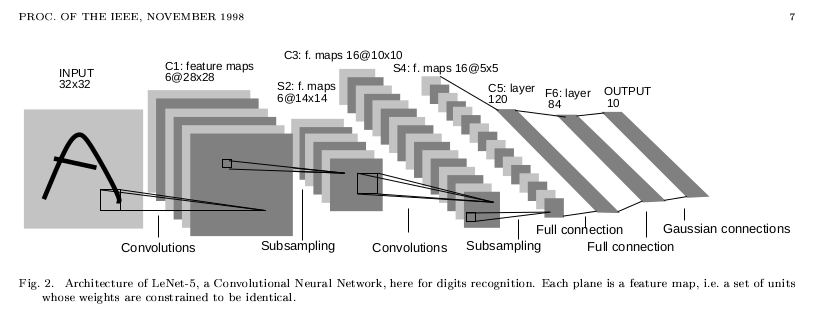
\includegraphics[width=0.8\linewidth]{ml-blog19-lenet5}
	\caption{สถาปัตยกรรมพื้นฐานของ Convolutional Neural Network (CNN)}
\end{figure}



\section*{Image classification (การจำแนกภาพ)}
\addcontentsline{toc}{section}{Image classification (การจำแนกภาพ)}

% ---------- Image classification ----------
\noindent{\bfseries\fontsize{16pt}{19.2pt}\selectfont }\par

\ThaiPara{\cite{superannotate2023imageclassification}~การจำแนกภาพคือการกำหนดป้ายกำกับให้รูปภาพจากชุดป้ายที่กำหนดล่วงหน้า
	ปัจจุบันโมเดลเชิงลึก โดยเฉพาะ CNN สามารถเรียนรู้คุณลักษณะสำคัญจากพิกเซลดิบแบบปลายทางถึงปลายทาง
	(\emph{end-to-end}) และส่งออกค่าความน่าจะเป็นของแต่ละคลาสได้อย่างมีประสิทธิภาพ}

\vspace{\baselineskip}

\begin{figure}[h]
	\centering
	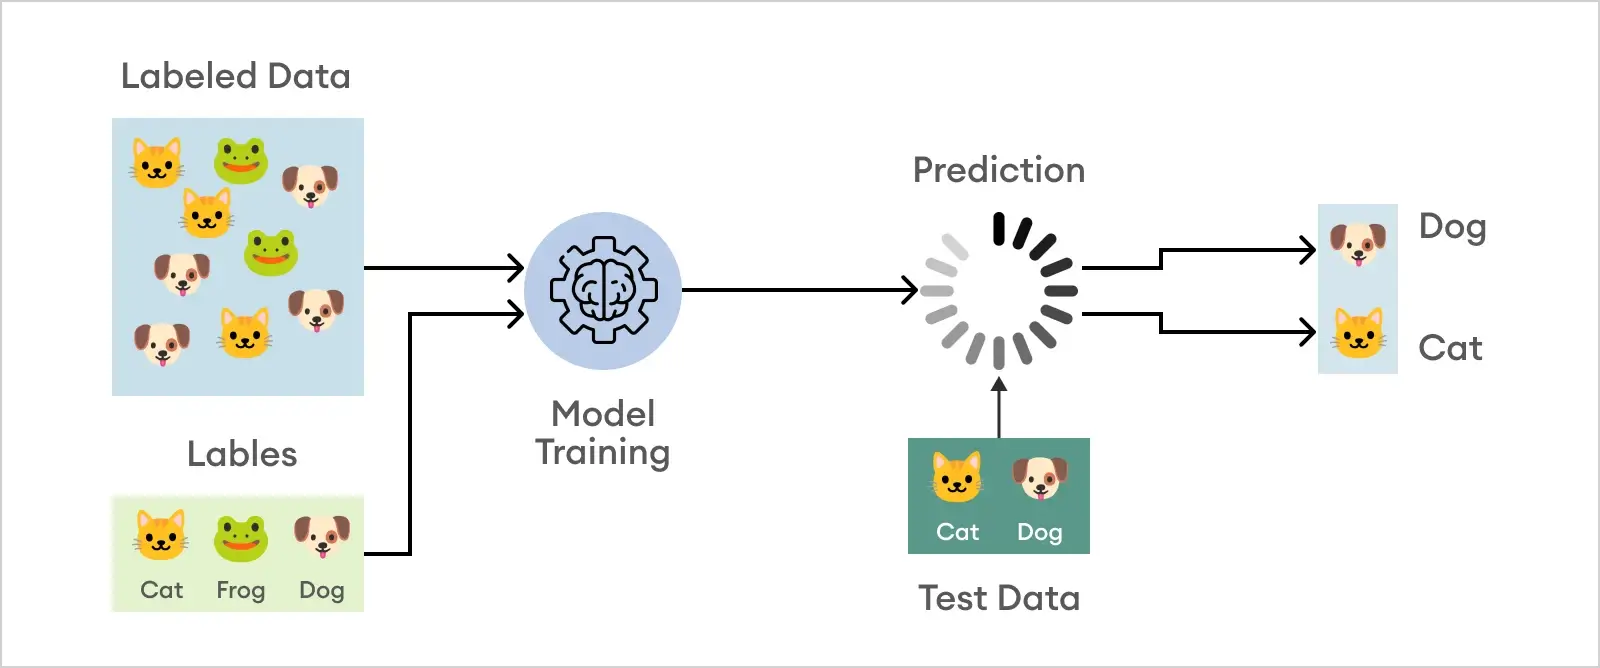
\includegraphics[width=0.8\linewidth]{png1}
	\caption{สถาปัตยกรรมพื้นฐานของการจำแนกภาพ}
\end{figure}

\par\endgroup
\clearpage
%================== จบ chapter2_1.tex ====================
}{}
	\IfFileExists{Chapter2_3.tex}{%==================== chapter2_3.tex ====================

\clearpage
\thispagestyle{plain}

\begingroup
\fontsize{16pt}{19.2pt}\selectfont
\justifying
\XeTeXlinebreakskip=0pt plus 1pt minus 0.5pt
\setlength{\parindent}{1.5cm}
\setlength{\parskip}{0pt}

% ---------- การออกแบบเว็บไซต์ที่รองรับการใช้งานบนทุกขนาดของหน้าจอ ----------
\section*{การออกแบบเว็บไซต์ที่รองรับการใช้งานบนทุกขนาดของหน้าจอ (Responsive web design)}
\addcontentsline{toc}{section}{การออกแบบเว็บไซต์ที่รองรับการใช้งานบนทุกขนาดของหน้าจอ (Responsive web design)}

\indent \cite{kinsta2024responsive} การออกแบบเว็บให้รองรับอุปกรณ์หลายชนิด (มือ ถือ แท็บเล็ต เดสก์ท็อป) ด้วยที่อยู่เว็บ
และโค้ดชุดเดียวโดยเลย์เอาต์ปรับตัวตามขนาดหน้าจออัตโนมัติช่วยคงประสบการณ์ใช้งานที่สม่ำเสมอ

\begin{figure}[h]
	\centering
	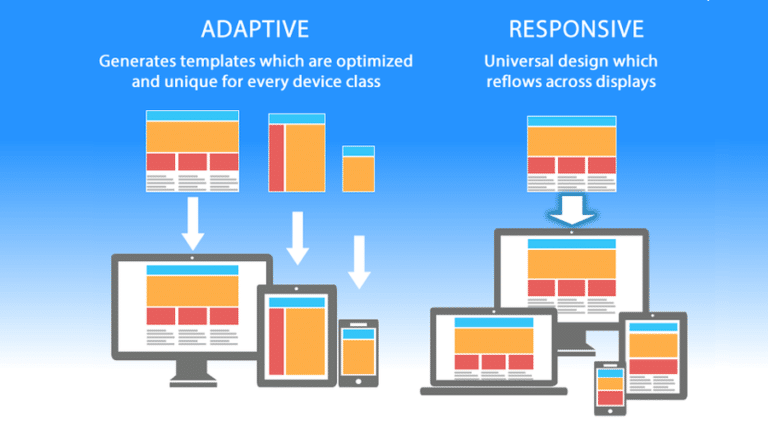
\includegraphics[width=0.8\linewidth]{responsive-adaptive-design-768x425}
	\caption{ภาพตัวอย่าง Responsive web design}
\end{figure}


% ---------- การออกแบบเว็บไซต์ที่รองรับการใช้งานบนทุกขนาดของหน้าจอ ----------

\section*{วงจรการพัฒนาซอฟต์แวร์}
\addcontentsline{toc}{section}{วงจรการพัฒนาซอฟต์แวร์}

\indent วงจรการพัฒนาซอฟต์แวร์ (Software Development Life Cycle: SDLC) มักแบ่งเป็น 6
ขั้นตอน ดังนี้

\begin{enumerate}
	\item \textbf{การวางแผน (Planning)} กำหนดเวลา ขอบเขต ทรัพยากร ผู้มีส่วนเกี่ยวข้อง และความเสี่ยง
	\item \textbf{เก็บรวบรวมและวิเคราะห์ความต้องการ (Requirements)} รวบรวมและทบทวนความต้องการของผู้ใช้/ระบบ
	\item \textbf{ออกแบบซอฟต์แวร์ (Design)} สถาปัตยกรรม ฐานข้อมูล UI/UX ความปลอดภัย เครือข่าย ฯลฯ
	\item \textbf{พัฒนา (Development)} พัฒนาแต่ละฟีเจอร์และรวมเป็นระบบตามดีไซน์
	\item \textbf{ทดสอบ (Testing)} สร้าง Test case ตรวจสอบตาม Requirement และใช้ Automated test ตามความเหมาะสม
	\item \textbf{บำรุงรักษา (Operations \& Maintenance)} เผยแพร่ แก้ไขบั๊ก เพิ่มฟีเจอร์และปรับปรุง คุณภาพอย่างต่อเนื่อง
\end{enumerate}}{}
	\IfFileExists{Chapter2_4.tex}{%==================== chapter2_4.tex ====================

\clearpage
\thispagestyle{plain}

\begingroup
\fontsize{16pt}{19.2pt}\selectfont
\justifying
\XeTeXlinebreakskip=0pt plus 1pt minus 0.5pt
\setlength{\parindent}{1.5cm}
\setlength{\parskip}{0pt}

% ---------- การพัฒนาเว็บแอปพลิเคชัน ----------
\noindent{\bfseries\fontsize{16pt}{19.2pt}\selectfont การพัฒนาเว็บแอปพลิเคชัน}\par

\ThaiPara{กระบวนการหลัก ได้แก่ การกำหนดแนวคิดและเป้าหมาย การวิเคราะห์ความต้องการ
	การออกแบบ UX/UI การทำต้นแบบ การพัฒนา (Front-end/Back-end) การทดสอบ
	(การใช้งาน ความปลอดภัย ประสิทธิภาพ) และการเผยแพร่ พร้อมดูแลปรับปรุงตามผลตอบรับของผู้ใช้}

\vspace{\baselineskip}

% ---------- งานวิจัยที่เกี่ยวข้อง ----------
\noindent{\bfseries\fontsize{16pt}{19.2pt}\selectfont งานวิจัยที่เกี่ยวข้อง}\par

\indent {ตัวอย่างประเด็นที่เกี่ยวข้อง เช่น 
	 งานวิจัยเกี่ยวกับการจำแนกภาพขวดแบบเซ็ตเปิดด้วยโครงข่ายประสาทเทียมแบบคอนโวลูชัน (Convolutional Neural Network หรือ CNN) โดย ศุภณัฐ จินตวัฒน์สกุล \cite{jintawatsakoon2019openset} มีวัตถุประสงค์หลักในการพัฒนาโมเดลที่สามารถจำแนกประเภทของขวดที่เปิดแล้วได้อย่างมีประสิทธิภาพ โดยการใช้เทคนิค Deep Learning เพื่อวิเคราะห์และประมวลผลภาพที่ถ่ายในสภาพแวดล้อมต่าง ๆ ในงานวิจัยนี้ ผู้วิจัยได้เสนอการใช้โครงข่ายประสาทเทียมแบบคอนโวลูชันซึ่งสามารถดึงคุณลักษณะสำคัญจากภาพ เช่น รูปร่าง สี และลวดลายของขวด โดยใช้ภาษาPython ร่วมกับไลบรารี TensorFlow เพื่อพัฒนาและฝึกสอนโมเดล การใช้ชุดข้อมูลที่มีภาพของขวดแบบเซ็ตเปิดที่ติดป้ายกำกับช่วยให้โมเดลสามารถเรียนรู้และปรับปรุงความแม่นยำในการจำแนกประเภทได้ ผลลัพธ์จากการทดลองแสดงให้เห็นว่าโมเดลที่พัฒนาขึ้นมีค่าความแม่นยำสูงในการจำแนกประเภทขวดเปิด ซึ่งสามารถนำไปประยุกต์ใช้ในหลายสาขา เช่น การควบคุมคุณภาพในอุตสาหกรรม หรือการจัดการขวดในระบบอัตโนมัติ ดังนั้นงานวิจัยนี้จึงมีความสำคัญในการพัฒนาเทคโนโลยี   การจำแนกภาพที่มีประสิทธิภาพและช่วยส่งเสริมการใช้งานในวงกว้าง.งานวิจัยเกี่ยวกับ "Responsive Portfolio Website Using React" \cite{muksikarat2016rwd} มีวัตถุประสงค์หลักในการพัฒนาเว็บไซต์พอร์ตโฟลิโอที่สามารถปรับตัวให้เข้ากับอุปกรณ์ต่าง ๆ ได้อย่างมีประสิทธิภาพ เช่นโทรศัพท์มือถือ แท็บเล็ต และคอมพิวเตอร์ โดยใช้เทคโนโลยี React ซึ่งเป็นไลบรารี Java Scriptที่นิยมในการสร้างส่วนประกอบที่มีความโต้ตอบสูง การเลือกใช้ React ช่วยให้การพัฒนาเว็บไซต์สามารถแบ่งแยกส่วนประกอบต่าง ๆ ได้ง่ายและทำให้โค้ดมีความเรียบร้อยและสามารถดูแลรักษาได้ง่ายขึ้น ในกระบวนการพัฒนา Siva Rama Lingham N และคณะ \cite{10425667} ได้ใช้ CSS และCSS Frameworks เช่น Bootstrap หรือ Tailwind CSS เพื่อสร้างเลย์เอาต์ที่ตอบสนองต่อการเปลี่ยนแปลงขนาดหน้าจอ โดยสามารถแสดงข้อมูลได้อย่างเหมาะสมและมีความน่าสนใจในทุกอุปกรณ์ นอกจากนี้ยังมีการใช้ JavaScript เพื่อเพิ่มการโต้ตอบระหว่างผู้ใช้กับเว็บไซต์ เช่น การจัดการสถานะของข้อมูล การตอบสนองต่อการกระทำของผู้ใช้ และการนำเสนอข้อมูลในรูปแบบที่น่าสนใจ ผลลัพธ์ที่ได้จากงานวิจัยนี้คือเว็บไซต์พอร์ตโฟลิโอที่ไม่เพียงแต่มีความสวยงามและใช้งานง่าย แต่ยังสามารถแสดงผลงานและข้อมูลของผู้ใช้ได้อย่างมีประสิทธิภาพในทุกแพลตฟอร์ม เว็บไซต์นี้ช่วยให้ผู้ใช้สามารถนำเสนอผลงานของตนได้อย่างมีสไตล์ และเป็นเครื่องมือที่มีประโยชน์ในการสร้างภาพลักษณ์ที่ดีในสายงานที่ตนสนใจ โดยรวมแล้วงานวิจัยนี้มีความสำคัญในการพัฒนาเทคโนโลยีเว็บที่ตอบสนองความต้องการของผู้ใช้ในยุคดิจิทัลที่มีการเปลี่ยนแปลงอย่างรวดเร็ว 
	 
	 \newpage 
	 
	 R.Archana and P.S. Eliahim Leevaraj \cite{8016501} งานวิจัยนี้สำรวจและประเมินโมเดลการเรียนรู้เชิง ลึก (Deep Learning) ในการประมวลผลภาพดิจิทัล เช่น การลดสัญญาณรบกวน การเพิ่มคุณภาพภาพ การ แบ่งส่วน การสกัดคุณลักษณะ และการจำแนกประเภท โดยเปรียบเทียบกับวิธีการประมวลผลภาพแบบดั้งเดิม โดยใช้ เทคนิคการประมวลผลภาพแบบดั้งเดิม เช่น การปรับความคมชัด การกรองสัญญาณรบกวน และการ แบ่งส่วนภาพ รวมถึงการใช้โมเดลการเรียนรู้เชิงลึก เช่น Convolutional Neural Networks (CNNs) และ Recurrent Neural Networks (RNNs) เพื่อเพิ่มประสิทธิภาพในการประมวลผลภาพ โดยมี 4 ขั้นตอน ได้แก่ 1.การเตรียมรูปภาพ เป็นการลดสัญญาณรบกวนและเพิ่มคุณภาพของรูป 2. การแบ่งส่วนภาพ เป็นการแยก ภาพออกเป็นส่วนๆ ตามลักษณะเฉพาะ 3.การสกัดคุณลักษณะ เป็นการดึงข้อมูลสำคัญจากภาพ 4.การจำแยก ประเภท เป็นการจัดหมวดหมู่ภาพตามเนื้อหา ผลลัพธ์ของงานวิจัยนี้แสดงให้เห็นว่าโมเดล DeepLabV3 และ U-Net มีความแม่นยำสูงกว่า FCN ในการแบ่งส่วนภาพจากมุมมองด้านบน ซึ่งมีความสำคัญในหลายๆ การใช้ งาน เช่น การเฝ้าระวัง การตรวจสอบฝูงชน และการโต้ตอบระหว่างมนุษย์กับคอมพิวเตอร์.}
	 
	

}{}
	
	% บทที่ 3 (ใช้หน้าใน Chapter3.tex เป็นหน้าบท)
	\thispagestyle{plain}
	\IfFileExists{Chapter3.tex}{%==================== chapter3.tex ====================

\clearpage
\thispagestyle{empty}

\begingroup
% เนื้อหาบท: 16pt baseline ~19.2pt ตามสเปกเล่ม
\fontsize{16pt}{19.2pt}\selectfont
\justifying
\XeTeXlinebreakskip=0pt plus 1pt minus 0.5pt
\setlength{\parindent}{1.5cm}
\setlength{\parskip}{0pt}

% ---------- หัวบท + เขียนสารบัญบทก่อนหัวข้อย่อย ----------
\phantomsection
\addcontentsline{toc}{chapter}{บทที่ 3 วิธีดำเนินงานวิจัย}
\begin{center}
	{\bfseries\fontsize{18pt}{21.6pt}\selectfont บทที่ 3}
\end{center}

\vspace{\baselineskip}

% ---------- ชื่อบท (วิธีดำเนินงานวิจัย) ----------
\begin{center}
	{\bfseries\fontsize{18pt}{21.6pt}\selectfont วิธีดำเนินงานวิจัย}
\end{center}

\vspace{\baselineskip}

% ---------- หัวข้อใหญ่ (ชิดซ้าย, หนา 16pt) ----------
\section*{การวิเคราะห์และการออกแบบระบบ}
\addcontentsline{toc}{section}{การวิเคราะห์และการออกแบบระบบ}

% ---------- เนื้อหา (จัดกระจายแบบไทย, ย่อหน้าแรก 1.5 ซม.) ----------
\indent ในการพัฒนาระบบเว็บแอปพลิเคชันศูนย์รวมการจัดประกวดปลากัดไทยนั้นจำเป็นต้องมีการ
ออกแบบระบบเพื่อชี้ให้เห็นโครงสร้างและหลักการทำงานของโครงงานนี้โดยผู้จัดทำได้ศึกษาค้นคว้า
และวิเคราะห์ความต้องการขิงผู้ใช้งานระบบจากนั้นได้นำรายละเอียดที่ได้จากการศึกษาและวิเคราะห์
นำมาออกแบบระบบซึ่งสามารถแบ่งออกเป็น

% ตั้งค่าให้เหมือนสเปกเดิมทุกบท
\setlength{\LoneLabelSep}{0.5em}
\settowidth{\LoneLabelWidth}{9.}
\setlength{\LoneContentCol}{\dimexpr 1.5cm + \LoneLabelWidth + \LoneLabelSep\relax}

\setlength{\LtwoLabelSep}{0.5em}
\settowidth{\LtwoLabelWidth}{9.9.}
\setlength{\ExtraAlign}{-2.8em}

% ระดับ 1: อินเดนต์ 1.5 ซม.
\setlist[enumerate,1]{%
	label=\arabic*., align=left,
	leftmargin=1.5cm, labelindent=0pt,
	labelwidth=\LoneLabelWidth, labelsep=\LoneLabelSep,
	itemsep=0pt, topsep=0.5\baselineskip
}

\begin{enumerate}
	\item Use Case Diagram
	\item Entity-Relation Diagram
	\item Class Diagram
	\item Sequence Diagram
	\item Activity Diagram
	\item Interface
\end{enumerate}

\clearpage}{}
	\IfFileExists{Chapter3_1.tex}{%==================== chapter3_1.tex ====================

\clearpage
\thispagestyle{plain}

\begingroup
\fontsize{16pt}{19.2pt}\selectfont
\justifying
\XeTeXlinebreakskip=0pt plus 1pt minus 0.5pt
\setlength{\parindent}{1.5cm}
\setlength{\parskip}{0pt}

% ---------- หัวข้อใหญ่ (ชิดซ้าย, หนา 16pt) ----------

\section*{Use Case Diagram}
\addcontentsline{toc}{section}{Use Case Diagram}

% ---------- เนื้อหา (จัดกระจายแบบไทย, ย่อหน้าแรก 1.5 ซม.) ----------
\indent Use Case Diagram ที่เป็นการจำลองการทำงานของผู้เข้าประกวดผู้เชี่ยวชาญและฝ่าย
ประชาสัมพันธ์ซึ่งจะเห็นได้ว่าระบบนี้ประกอบไปด้วย 27 Use Case Diagram คือ

\vspace{\baselineskip}

\begin{figure}[h]
	\centering
	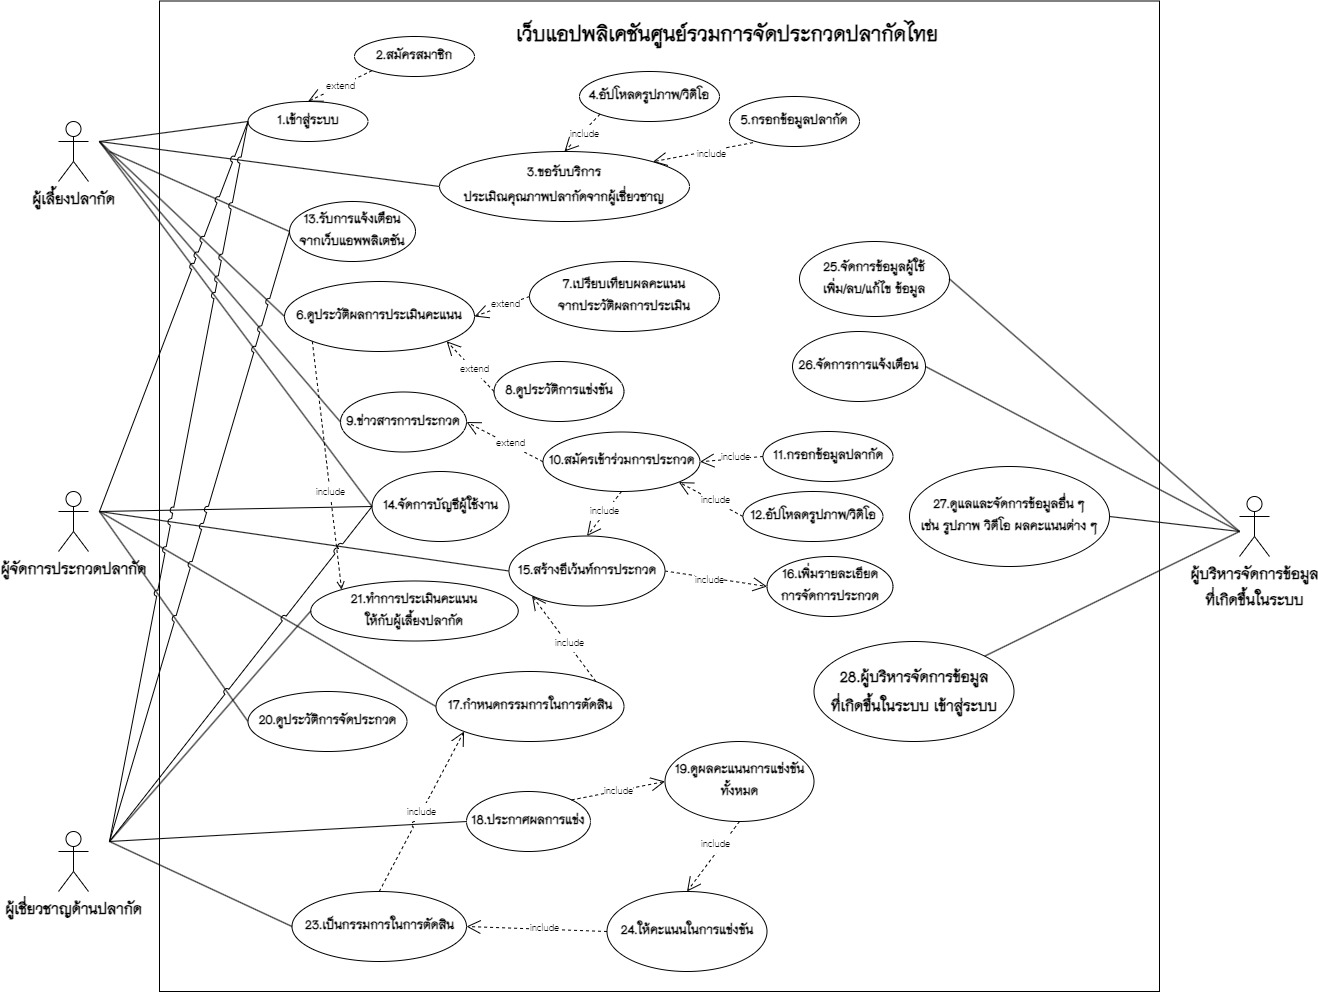
\includegraphics[width=0.8\linewidth]{Pasted image}
	\caption{Use Case ระบบเว็บแอปพลิเคชันศูนย์รวมการจัดประกวดปลากัดไทย}
\end{figure}

% ตั้งค่าให้เหมือนสเปกเดิมทุกบท
\setlength{\LoneLabelSep}{0.5em}
\settowidth{\LoneLabelWidth}{9.}
\setlength{\LoneContentCol}{\dimexpr 1.5cm + \LoneLabelWidth + \LoneLabelSep\relax}

\setlength{\LtwoLabelSep}{0.5em}
\settowidth{\LtwoLabelWidth}{9.9.}
\setlength{\ExtraAlign}{-2.8em}

% ระดับ 1: อินเดนต์ 1.5 ซม.
\setlist[enumerate,1]{%
	label=\arabic*., align=left,
	leftmargin=1.5cm, labelindent=0pt,
	labelwidth=\LoneLabelWidth, labelsep=\LoneLabelSep,
	itemsep=0pt, topsep=0.5\baselineskip
}

\begin{enumerate}
	\item Use Case: เข้าสู่ระบบ
	\item Use Case: สมัครสมาชิก
	\item Use Case: ขอรับบริการประเมินคุณภาพปลากัดจากผู้เชี่ยวชาญ
	\item Use Case: อัปโหลดรูปภาพ/วิดีโอ
	\item Use Case: กรอกข้อมูลปลากัด
	\item Use Case: ดูประวัติผลการประเมินคะแนน
	\item Use Case: เปรียบเทียบผลคะแนนจากประวัติผลการประเมิน
	\item Use Case: ดูประวัติการแข่งขัน
	\item Use Case: ข่าวสารการประกวด
	\item Use Case: สมัครเข้าร่วมการประกวด
	\item Use Case: กรอกข้อมูลปลากัด
	\item Use Case: อัปโหลดรูปภาพ/วิดีโอ
	\item Use Case: รับการแจ้งเตือนจากเว็บแอปพลิเคชัน
	\item Use Case: จัดการบัญชีผู้ใช้งาน
	\item Use Case: สร้างอีเว้นท์การประกวด
	\item Use Case: เพิ่มรายรายละเอียดการจัดการประกวด
	\item Use Case: กำหนดกรรมการในการตัดสิน
	\item Use Case: ประกาศผลการแข่งขัน
	\item Use Case: ดูผลคะแนนการแข่งขันทั้งหมด
	\item Use Case: ดูประวัติการจัดประกวด
	\item Use Case: ให้บริการประเมินคุณภาพปลากัดทำการประเมินคะแนนให้กับผู้เลี้ยงปลากัด
	\item Use Case: เป็นกรรมการในการตัดสิน
	\item Use Case: ให้คะแนนในการแข่งขัน
	\item Use Case: จัดการข้อมูลผู้ใช้ เพิ่ม/ลบ/แก้ไข ข้อมูล
	\item Use Case: จัดการการแจ้งเตือน
	\item Use Case: ดูแลและจัดการข้อมูลอื่นๆ เช่นรูปภาพ วิดีโอ ผลคะแนนต่างๆ
	\item Use Case: ผู้บริหารจัดการข้อมูลที่เกิดขึ้นในระบบ เข้าสู่ระบบ
\end{enumerate}

\vspace{\baselineskip}

% ================== Use Case: Login ==================
\begin{table}[h]
	\caption{Use Case สำหรับการเข้าสู่ระบบ}
	{\tablefont
		\setlength{\tabcolsep}{6pt}%
		\begin{tabularx}{\linewidth}{@{} >{\justifying\arraybackslash}X >{\raggedleft\arraybackslash}p{4.2cm} @{}}
			\Xhline{1.5pt}
			\textbf{Use Case Title:}\enspace เข้าสู่ระบบ & \UseCaseID[uc:login] \\
			\Xhline{0.5pt}
			\textbf{Primary Actor:}\enspace ผู้เลี้ยงปลากัด, ผู้จัดการประกวด, ผู้เชี่ยวชาญด้านปลากัด, ผู้บริหารจัดการข้อมูลที่เกิดขึ้นในระบบ & \\
			\Xhline{0.5pt}
			\textbf{Stakeholder Actor:}\enspace - & \\
			\Xhline{0.5pt}
			\textbf{Main Flow:}\enspace สามารถกรอก username และ password เข้าสู่ระบบใช้งานได้เลยกรณีมีบัญชีผู้ใช้งานอยู่แล้ว & \\
			\Xhline{0.5pt}
			\textbf{Exception Flow ที่ 1:}\enspace กรณีที่ผู้ใช้งานยังไม่มีบัญชีเข้าใช้งาน ระบบจะแจ้งเตือนให้ผู้ใช้สมัครสมาชิกก่อนเข้าใช้งานเว็บแอพพลิเคชัน & \\
			\Xhline{1.5pt}
		\end{tabularx}
	}
\end{table}
% =====================================================



\clearpage}{}
	\IfFileExists{Chapter3_2.tex}{%==================== chapter3_2.tex ====================

\clearpage
\thispagestyle{plain}

\begingroup
\fontsize{16pt}{19.2pt}\selectfont
\justifying
\XeTeXlinebreakskip=0pt plus 1pt minus 0.5pt
\setlength{\parindent}{1.5cm}
\setlength{\parskip}{0pt}

% ================== Use Case: Register ==================
\begin{table}[h]
	\caption{Use Case สมัครสมาชิก}
	{\tablefont
		\setlength{\tabcolsep}{6pt}%
		\begin{tabularx}{\linewidth}{@{} >{\justifying\arraybackslash}X >{\raggedleft\arraybackslash}p{4.2cm} @{}}
			\Xhline{1.5pt}
			\textbf{Use Case Title:}\enspace สมัครสมาชิก & \UseCaseID[uc:register] \\
			\Xhline{0.5pt}
			\textbf{Primary Actor:}\enspace ผู้เลี้ยงปลากัด, ผู้จัดการประกวด, ผู้เชี่ยวชาญด้านปลากัด & \\
			\Xhline{0.5pt}
			\textbf{Stakeholder Actor:}\enspace - & \\
			\Xhline{0.5pt}
			\textbf{Main Flow:}\enspace ผู้ใช้ที่ยังไม่มีบัญชีเข้าใช้งาน สามารถสมัครสมาชิกเพื่อเข้าใช้งานระบบได้ & \\
			\Xhline{0.5pt}
			\textbf{Exception Flow ที่ 1:}\enspace กรณีผู้ใช้กรอกข้อมูลไม่ครบถ้วนหรือไม่ตรงตามเงื่อนไข ระบบจะทำการแจ้งข้อความเตือน & \\
			\Xhline{0.5pt}
			\textbf{Exception Flow ที่ 2:}\enspace กรณีที่ผู้ใช้มีบัญชีอยู่แล้ว ระบบจะทำการแจ้งเตือนให้ทราบ & \\
			\Xhline{1.5pt}
		\end{tabularx}
	}
\end{table}
% =====================================================

% ================== Use Case ขอรับบริการประเมิณคุณภาพปลากัดจากผู้เชี่ยวชาญ ==================
\begin{table}[h]
	\caption{Use Case ขอรับบริการประเมิณคุณภาพปลากัดจากผู้เชี่ยวชาญ}
	{\tablefont
		\setlength{\tabcolsep}{6pt}%
		\begin{tabularx}{\linewidth}{@{} >{\justifying\arraybackslash}X >{\raggedleft\arraybackslash}p{4.2cm} @{}}
			\Xhline{1.5pt}
			\textbf{Use Case Title:}\enspace ขอรับบริการประเมิณคุณภาพปลากัดจากผู้เชี่ยวชาญ & \UseCaseID[uc:register] \\
			\Xhline{0.5pt}
			\textbf{Primary Actor:}\enspace ผู้เลี้ยงปลากัด & \\
			\Xhline{0.5pt}
			\textbf{Stakeholder Actor:}\enspace - & \\
			\Xhline{0.5pt}
			\textbf{Main Flow:}\enspace ผู้ใช้สามารถขอรับบริการประเมินคุณภาพปลากัดปลากัดเพื่อประประเมินคุณภาพปลากัดของผู้เลี้ยงได้
			จากผู้เชี่ยวชาญ & \\
			\Xhline{0.5pt}
			\textbf{Exception Flow ที่ 1:}\enspace ผู้ใช้ต้องทำการอัปโหลดข้อมูลเกี่ยวกับปลากัดเข้ามาก่อนถึงจะสามารถส่งไปให้ผู้เชี่ยวประเมินคุณภาพให้ได้ & \\
			\Xhline{1.5pt}
		\end{tabularx}
	}
\end{table}
% =====================================================

% ================== Use Case อัปโหลดรูปภาพ/วิดีโอ ==================
\begin{table}[h]
	\caption{Use Case อัปโหลดรูปภาพ/วิดีโอ}
	{\tablefont
		\setlength{\tabcolsep}{6pt}%
		\begin{tabularx}{\linewidth}{@{} >{\justifying\arraybackslash}X >{\raggedleft\arraybackslash}p{4.2cm} @{}}
			\Xhline{1.5pt}
			\textbf{Use Case Title:}\enspace อัปโหลดรูปภาพ/วิดีโอ & \UseCaseID[uc:register] \\
			\Xhline{0.5pt}
			\textbf{Primary Actor:}\enspace ผู้เลี้ยงปลากัด & \\
			\Xhline{0.5pt}
			\textbf{Stakeholder Actor:}\enspace - & \\
			\Xhline{0.5pt}
			\textbf{Main Flow:}\enspace ทำการเพิ่มรูปภาพ/วิดีโอ ลงบนเว็บแอพพลิเคชันเพื่อทำการประเมินผลคะแนนโดยวิธีการต่างๆ & \\
			\Xhline{1.5pt}
		\end{tabularx}
	}
\end{table}
% =====================================================

\clearpage}{}
	\IfFileExists{Chapter3_3.tex}{%==================== chapter3_3.tex ====================

\clearpage
\thispagestyle{plain}

\begingroup
\fontsize{16pt}{19.2pt}\selectfont
\justifying
\XeTeXlinebreakskip=0pt plus 1pt minus 0.5pt
\setlength{\parindent}{1.5cm}
\setlength{\parskip}{0pt}

% ================== Use Case กรอกข้อมูลปลากัด ==================
\begin{table}[h]
	\caption{Use Case กรอกข้อมูลปลากัด}
	{\tablefont
		\setlength{\tabcolsep}{6pt}%
		\begin{tabularx}{\linewidth}{@{} >{\justifying\arraybackslash}X >{\raggedleft\arraybackslash}p{4.2cm} @{}}
			\Xhline{1.5pt}
			\textbf{Use Case Title:}\enspace กรอกข้อมูลปลากัด & \UseCaseID[uc:register] \\
			\Xhline{0.5pt}
			\textbf{Primary Actor:}\enspace ผู้เลี้ยงปลากัด & \\
			\Xhline{0.5pt}
			\textbf{Stakeholder Actor:}\enspace - & \\
			\Xhline{0.5pt}
			\textbf{Main Flow:}\enspace ผู้ใช้ทำการกรอกรายละเอียดข้อมูลปลากัด เช่น ชื่อปลากัดอายุปลากัดประเภทปลากัด & \\
			\Xhline{1.5pt}
		\end{tabularx}
	}
\end{table}
% =====================================================

% ================== Use Case ดูประวัติผลการประเมินคะแนน ==================
\begin{table}[h]
	\caption{Use Case ดูประวัติผลการประเมินคะแนน}
	{\tablefont
		\setlength{\tabcolsep}{6pt}%
		\begin{tabularx}{\linewidth}{@{} >{\justifying\arraybackslash}X >{\raggedleft\arraybackslash}p{4.2cm} @{}}
			\Xhline{1.5pt}
			\textbf{Use Case Title:}\enspace ดูประวัติผลการประเมินคะแนน & \UseCaseID[uc:register] \\
			\Xhline{0.5pt}
			\textbf{Primary Actor:}\enspace ผู้เลี้ยงปลากัด & \\
			\Xhline{0.5pt}
			\textbf{Stakeholder Actor:}\enspace - & \\
			\Xhline{0.5pt}
			\textbf{Main Flow:}\enspace ผู้เลี้ยงปลากัดสามารถเข้าดูประวัคิการการประเมินได้ทั้งหมดที่ตนเองเคยได้ทำการประเมินผลไว้ & \\
			\Xhline{0.5pt}
			\textbf{Exception Flow ที่ 1:}\enspace จัดการการแจ้งเตือนและข้อมูลสำคัญของระบบ , ผู้ใช้สามารถทำการเปรียบทียบผลคะแนนจากปลาตัวอื่นหรือว่าปลาตัวเดียวกันที่เคยประเมินไว้ก่อนหน้านี้ & \\
			\Xhline{1.5pt}
		\end{tabularx}
	}
\end{table}
% =====================================================

% ================== Use Case เปรียบเทียบผลคะแนนจากประวัติการประเมิน ==================
\begin{table}[h]
	\caption{Use Case เปรียบเทียบผลคะแนนจากประวัติการประเมิน}
	{\tablefont
		\setlength{\tabcolsep}{6pt}%
		\begin{tabularx}{\linewidth}{@{} >{\justifying\arraybackslash}X >{\raggedleft\arraybackslash}p{4.2cm} @{}}
			\Xhline{1.5pt}
			\textbf{Use Case Title:}\enspace เปรียบเทียบผลคะแนนจากประวัติการประเมิน & \UseCaseID[uc:register] \\
			\Xhline{0.5pt}
			\textbf{Primary Actor:}\enspace ผู้เลี้ยงปลากัด & \\
			\Xhline{0.5pt}
			\textbf{Stakeholder Actor:}\enspace - & \\
			\Xhline{0.5pt}
			\textbf{Main Flow:}\enspace สามารถเปรียบเทียบผลคะแนนกับปลาตัวอื่น ๆ ได้หรือว่าจะเป็นปลาตัวเดียวกันก็ได้เช่นกัน
			เพื่อให้เห็นการวิวัฒนาการของปลา หรือ ความแตกตางระหว่างปลา 2 ตัว & \\
			\Xhline{1.5pt}
		\end{tabularx}
	}
\end{table}
% =====================================================
\clearpage
}{}
	\IfFileExists{Chapter3_4.tex}{%==================== chapter3_4.tex ====================

\clearpage
\thispagestyle{plain}

\begingroup
\fontsize{16pt}{19.2pt}\selectfont
\justifying
\XeTeXlinebreakskip=0pt plus 1pt minus 0.5pt
\setlength{\parindent}{1.5cm}
\setlength{\parskip}{0pt}

% ================== Use Case ดูประวัติการแข่งขัน ==================
\begin{table}[h]
	\caption{Use Case ดูประวัติการแข่งขัน}
	{\tablefont
		\setlength{\tabcolsep}{6pt}%
		\begin{tabularx}{\linewidth}{@{} >{\justifying\arraybackslash}X >{\raggedleft\arraybackslash}p{4.2cm} @{}}
			\Xhline{1.5pt}
			\textbf{Use Case Title:}\enspace ดูประวัติการแข่งขัน & \UseCaseID[uc:register] \\
			\Xhline{0.5pt}
			\textbf{Primary Actor:}\enspace ผู้เลี้ยงปลากัด & \\
			\Xhline{0.5pt}
			\textbf{Stakeholder Actor:}\enspace - & \\
			\Xhline{0.5pt}
			\textbf{Main Flow:}\enspace สามารถดูประวัติการเข้าร่วมการแข่งขันได้ทั้งหมด เพื่อดูว่าผู้เลี้ยงทำการแข่งขันไปทั้งหมดกี่ครั้งแล้ว & \\
			\Xhline{1.5pt}
		\end{tabularx}
	}
\end{table}
% =====================================================

% ================== Use Case ข่าวสารการประกวด ==================
\begin{table}[h]
	\caption{Use Case ข่าวสารการประกวด}
	{\tablefont
		\setlength{\tabcolsep}{6pt}%
		\begin{tabularx}{\linewidth}{@{} >{\justifying\arraybackslash}X >{\raggedleft\arraybackslash}p{4.2cm} @{}}
			\Xhline{1.5pt}
			\textbf{Use Case Title:}\enspace ข่าวสารการประกวด & \UseCaseID[uc:register] \\
			\Xhline{0.5pt}
			\textbf{Primary Actor:}\enspace ผู้เลี้ยงปลากัด, ผู้จัดการประกวด, ผู้เชี่ยวชาญด้านปลากัด & \\
			\Xhline{0.5pt}
			\textbf{Stakeholder Actor:}\enspace - & \\
			\Xhline{0.5pt}
			\textbf{Main Flow:}\enspace ข้าชมข่าวสารการประกวดต่างๆในเว็บ แต่ละข่าวสารอาจมีการรับสมัครเข้าร่วมการแข่งขัน & \\
			\Xhline{0.5pt}
			\textbf{Exception Flow ที่ 1:}\enspace สามารถกดสมัครเข้าร่วมการประกวดปลากัดได้ & \\
			\Xhline{0.5pt}
			\textbf{Exception Flow ที่ 2:}\enspace การที่จะสมัครเข้าร่วมกันแข่งขันได้นั้น จะต้องมีอีเว้นท์การประกวดก่อนถึงจะเข้าร่วมการแข่งได้ & \\
			\Xhline{1.5pt}
		\end{tabularx}
	}
\end{table}
% =====================================================

% ================== Use Case สมัครเข้าร่วมการประกวด ==================
\begin{table}[h]
	\caption{Use Case สมัครเข้าร่วมการประกวด}
	{\tablefont
		\setlength{\tabcolsep}{6pt}%
		\begin{tabularx}{\linewidth}{@{} >{\justifying\arraybackslash}X >{\raggedleft\arraybackslash}p{4.2cm} @{}}
			\Xhline{1.5pt}
			\textbf{Use Case Title:}\enspace สมัครเข้าร่วมการประกวด & \UseCaseID[uc:register] \\
			\Xhline{0.5pt}
			\textbf{Primary Actor:}\enspace ผู้เลี้ยงปลากัด & \\
			\Xhline{0.5pt}
			\textbf{Stakeholder Actor:}\enspace - & \\
			\Xhline{0.5pt}
			\textbf{Main Flow:}\enspace สามารถกดสมัครเข้าร่วมการประกวดปลากัด ในกิจกรรมนั้นๆได้ & \\
			\Xhline{0.5pt}
			\textbf{Exception Flow ที่ 1:}\enspace สามารถกดสมัครเข้าร่วมการประกวดปลากัดได้ & \\
			\Xhline{0.5pt}
			\textbf{Exception Flow ที่ 2:}\enspace การที่จะสมัครเข้าร่วมกันแข่งขันได้นั้น จะต้องมีอีเว้นท์การประกวดก่อนถึงจะเข้าร่วมการแข่ง
			ได้ & \\
			\Xhline{1.5pt}
		\end{tabularx}
	}
\end{table}
% =====================================================
\clearpage}{}
	\IfFileExists{Chapter3_5.tex}{%==================== chapter3_6.tex ====================

\clearpage
\thispagestyle{plain}

\begingroup
\fontsize{16pt}{19.2pt}\selectfont
\justifying
\XeTeXlinebreakskip=0pt plus 1pt minus 0.5pt
\setlength{\parindent}{1.5cm}
\setlength{\parskip}{0pt}

% ================== Use Case กรอกข้อมูลปลากัด ==================
\begin{table}[h]
	\caption{Use Case กรอกข้อมูลปลากัด}
	{\tablefont
		\setlength{\tabcolsep}{6pt}%
		\begin{tabularx}{\linewidth}{@{} >{\justifying\arraybackslash}X >{\raggedleft\arraybackslash}p{4.2cm} @{}}
			\Xhline{1.5pt}
			\textbf{Use Case Title:}\enspace กรอกข้อมูลปลากัด & \UseCaseID[uc:register] \\
			\Xhline{0.5pt}
			\textbf{Primary Actor:}\enspace ผู้เลี้ยงปลากัด & \\
			\Xhline{0.5pt}
			\textbf{Stakeholder Actor:}\enspace - & \\
			\Xhline{0.5pt}
			\textbf{Main Flow:}\enspace กรอกรายละเอียดข้อมูลปลากัดเพื่อสมัครเข้าร่วมการแข่งขันปลากัด & \\
			\Xhline{1.5pt}
		\end{tabularx}
	}
\end{table}
% =====================================================

% ================== Use Case อัปโหลดรูปภาพ/วิดีโอ ==================
\begin{table}[h]
	\caption{Use Case อัปโหลดรูปภาพ/วิดีโอ}
	{\tablefont
		\setlength{\tabcolsep}{6pt}%
		\begin{tabularx}{\linewidth}{@{} >{\justifying\arraybackslash}X >{\raggedleft\arraybackslash}p{4.2cm} @{}}
			\Xhline{1.5pt}
			\textbf{Use Case Title:}\enspace อัปโหลดรูปภาพ/วิดีโอ & \UseCaseID[uc:register] \\
			\Xhline{0.5pt}
			\textbf{Primary Actor:}\enspace ผู้เลี้ยงปลากัด & \\
			\Xhline{0.5pt}
			\textbf{Stakeholder Actor:}\enspace - & \\
			\Xhline{0.5pt}
			\textbf{Main Flow:}\enspace ทำการอัปโหลดรูปภาพ/วิดีโอ ของปลากัดเพื่อสมัคนเข้าประกวด & \\
			\Xhline{1.5pt}
		\end{tabularx}
	}
\end{table}
% =====================================================

% ================== Use Case รับการแจ้งเตือนจากระบบ ==================
\begin{table}[h]
	\caption{Use Case รับการแจ้งเตือนจากระบบ}
	{\tablefont
		\setlength{\tabcolsep}{6pt}%
		\begin{tabularx}{\linewidth}{@{} >{\justifying\arraybackslash}X >{\raggedleft\arraybackslash}p{4.2cm} @{}}
			\Xhline{1.5pt}
			\textbf{Use Case Title:}\enspace รับการแจ้งเตือนจากระบบ & \UseCaseID[uc:register] \\
			\Xhline{0.5pt}
			\textbf{Primary Actor:}\enspace ผู้เลี้ยงปลากัด, ผู้จัดการประกวด, ผู้เชี่ยวชาญด้านปลากัด & \\
			\Xhline{0.5pt}
			\textbf{Stakeholder Actor:}\enspace - & \\
			\Xhline{0.5pt}
			\textbf{Main Flow:}\enspace การแจ้งเตือนการแข่งขัน การแจ้งเตือนเกี่ยวกับข่าวสารการแข่งขันต่าง ๆ & \\
			\Xhline{1.5pt}
		\end{tabularx}
	}
\end{table}
% =====================================================

\clearpage}{}
	\IfFileExists{Chapter3_6.tex}{%==================== chapter3_2.tex ====================

\clearpage
\thispagestyle{plain}

\begingroup
\fontsize{16pt}{19.2pt}\selectfont
\justifying
\XeTeXlinebreakskip=0pt plus 1pt minus 0.5pt
\setlength{\parindent}{1.5cm}
\setlength{\parskip}{0pt}

% ================== Use Case จัดการบัญชีผู้ใช้งาน ==================
\begin{table}[h]
	\caption{Use Case จัดการบัญชีผู้ใช้งาน}
	{\tablefont
		\setlength{\tabcolsep}{6pt}%
		\begin{tabularx}{\linewidth}{@{} >{\justifying\arraybackslash}X >{\raggedleft\arraybackslash}p{4.2cm} @{}}
			\Xhline{1.5pt}
			\textbf{Use Case Title:}\enspace จัดการบัญชีผู้ใช้งาน & \UseCaseID[uc:register] \\
			\Xhline{0.5pt}
			\textbf{Primary Actor:}\enspace ผู้เลี้ยงปลากัด, ผู้จัดการประกวด, ผู้เชี่ยวชาญด้านปลากัด & \\
			\Xhline{0.5pt}
			\textbf{Stakeholder Actor:}\enspace - & \\
			\Xhline{0.5pt}
			\textbf{Main Flow:}\enspace สามารถทำการจัดการบัญชี ผู้ ใช้ งานของตนเองได้ เช่น แก้ไขรูป โปรไฟล์ แก้ไขชื่อ-สกุล แก้ ไข
			ยูสเซอร์เนม แก้ไขพาสเวิร์ด & \\
			\Xhline{1.5pt}
		\end{tabularx}
	}
\end{table}
% =====================================================

% ================== Use Case สร้างอีเว้นท์การประกวด ==================
\begin{table}[h]
	\caption{Use Case สร้างอีเว้นท์การประกวด}
	{\tablefont
		\setlength{\tabcolsep}{6pt}%
		\begin{tabularx}{\linewidth}{@{} >{\justifying\arraybackslash}X >{\raggedleft\arraybackslash}p{4.2cm} @{}}
			\Xhline{1.5pt}
			\textbf{Use Case Title:}\enspace สร้างอีเว้นท์การประกวด & \UseCaseID[uc:register] \\
			\Xhline{0.5pt}
			\textbf{Primary Actor:}\enspace ผู้จัดการประกวด & \\
			\Xhline{0.5pt}
			\textbf{Stakeholder Actor:}\enspace - & \\
			\Xhline{0.5pt}
			\textbf{Main Flow:}\enspace ทำการสร้างอีเว้นท์การประกวดเพื่อจัดการแข่งขันการประกวดปลากัด
			ยูสเซอร์เนม แก้ไขพาสเวิร์ด & \\
			\Xhline{0.5pt}
			\textbf{Exception Flow ที่ 1:}\enspace ผู้จัดการประกวดปลากัดจะต้องทำการเพิ่มรายละเอียดข้อมูลต่างๆที่เกี่ยวข้องกับการแข่งขัน & \\
			\Xhline{1.5pt}
		\end{tabularx}
	}
\end{table}
% =====================================================

% ================== Use Case เพิ่มรายละเอียดการจัดการประกวด ==================
\begin{table}[h]
	\caption{Use Case เพิ่มรายละเอียดการจัดการประกวด}
	{\tablefont
		\setlength{\tabcolsep}{6pt}%
		\begin{tabularx}{\linewidth}{@{} >{\justifying\arraybackslash}X >{\raggedleft\arraybackslash}p{4.2cm} @{}}
			\Xhline{1.5pt}
			\textbf{Use Case Title:}\enspace เพิ่มรายละเอียดการจัดการประกวด & \UseCaseID[uc:register] \\
			\Xhline{0.5pt}
			\textbf{Primary Actor:}\enspace ผู้จัดการประกวด & \\
			\Xhline{0.5pt}
			\textbf{Stakeholder Actor:}\enspace - & \\
			\Xhline{0.5pt}
			\textbf{Main Flow:}\enspace พิ่ มรายละเอียดข้อมูล เกี่ยวกับ การประกวดต่างๆ เพื่อ ให้ ผู้ เลี้ยงทราบถึง รายละเอียดขอมูล
			ต่างๆในการแข่งขันครั้งนั้น & \\
			\Xhline{0.5pt}
			\textbf{Exception Flow ที่ 1:}\enspace ผู้จัดการประกวดปลากัดจะต้องทำการเพิ่มรายละเอียดข้อมูลต่างๆที่เกี่ยวข้องกับการแข่งขัน & \\
			\Xhline{1.5pt}
		\end{tabularx}
	}
\end{table}
% =====================================================

\clearpage}{}
	\IfFileExists{Chapter3_7.tex}{%==================== chapter3_7.tex ====================

\clearpage
\thispagestyle{plain}

\begingroup
\fontsize{16pt}{19.2pt}\selectfont
\justifying
\XeTeXlinebreakskip=0pt plus 1pt minus 0.5pt
\setlength{\parindent}{1.5cm}
\setlength{\parskip}{0pt}

% ================== Use Case กำหนดกรรมการในการตัดสิน ==================
\begin{table}[h]
	\caption{Use Case กำหนดกรรมการในการตัดสิน}
	{\tablefont
		\setlength{\tabcolsep}{6pt}%
		\begin{tabularx}{\linewidth}{@{} >{\justifying\arraybackslash}X >{\raggedleft\arraybackslash}p{4.2cm} @{}}
			\Xhline{1.5pt}
			\textbf{Use Case Title:}\enspace กำหนดกรรมการในการตัดสิน & \UseCaseID[uc:register] \\
			\Xhline{0.5pt}
			\textbf{Primary Actor:}\enspace ผู้จัดการประกวด & \\
			\Xhline{0.5pt}
			\textbf{Stakeholder Actor:}\enspace - & \\
			\Xhline{0.5pt}
			\textbf{Main Flow:}\enspace กำหนดผู้เชี่ยวชาญเพื่อให้มาเป็นกรรมการในการตัดสินในแต่ ครั้งและกำหนด จำนวนกรรมการว่ากรรมการในการตัดสินการแข่งขันนี้ทั้งหมดกี่คน & \\
			\Xhline{1.5pt}
		\end{tabularx}
	}
\end{table}
% =====================================================

% ================== Use Case ประกาศผลการแข่งขัน ==================
\begin{table}[h]
	\caption{Use Case ประกาศผลการแข่งขัน}
	{\tablefont
		\setlength{\tabcolsep}{6pt}%
		\begin{tabularx}{\linewidth}{@{} >{\justifying\arraybackslash}X >{\raggedleft\arraybackslash}p{4.2cm} @{}}
			\Xhline{1.5pt}
			\textbf{Use Case Title:}\enspace ประกาศผลการแข่งขัน & \UseCaseID[uc:register] \\
			\Xhline{0.5pt}
			\textbf{Primary Actor:}\enspace ผู้จัดการประกวด & \\
			\Xhline{0.5pt}
			\textbf{Stakeholder Actor:}\enspace - & \\
			\Xhline{0.5pt}
			\textbf{Main Flow:}\enspace ทำการประกาศผลคะแนนการแข่งขันตามที่กรรมการได้ให้คะแนนไว้ & \\
			\Xhline{0.5pt}
			\textbf{Exception Flow ที่ 1:}\enspace กรรมการต้องทำการให้คะแนนการประเมินก่อนถึงจะสามารถประกาศผลการแข่งได้ & \\
			\Xhline{1.5pt}
		\end{tabularx}
	}
\end{table}
% =====================================================

% ================== Use Case ดูผลคะแนนการแข่งขัน ==================
\begin{table}[h]
	\caption{Use Case ดูผลคะแนนการแข่งขัน}
	{\tablefont
		\setlength{\tabcolsep}{6pt}%
		\begin{tabularx}{\linewidth}{@{} >{\justifying\arraybackslash}X >{\raggedleft\arraybackslash}p{4.2cm} @{}}
			\Xhline{1.5pt}
			\textbf{Use Case Title:}\enspace ดูผลคะแนนการแข่งขัน & \UseCaseID[uc:register] \\
			\Xhline{0.5pt}
			\textbf{Primary Actor:}\enspace ผู้จัดการประกวด & \\
			\Xhline{0.5pt}
			\textbf{Stakeholder Actor:}\enspace - & \\
			\Xhline{0.5pt}
			\textbf{Main Flow:}\enspace สามารถดูผลคะแนนที่กรรมการทำการให้คะแนน & \\
			\Xhline{0.5pt}
			\textbf{Exception Flow ที่ 1:}\enspace ผู้จัดการประกวดต้องทราบผลคะแนนที่กรรมให้คะแนนได้ก่อนถึงจะทำการประกาศผู้ทื่ชนะ
			ในการแข่งขันนั้นได้ & \\
			\Xhline{1.5pt}
		\end{tabularx}
	}
\end{table}
% =====================================================

\clearpage}{}
	\IfFileExists{Chapter3_8.tex}{%==================== chapter3_8.tex ====================

\clearpage
\thispagestyle{plain}

\begingroup
\fontsize{16pt}{19.2pt}\selectfont
\justifying
\XeTeXlinebreakskip=0pt plus 1pt minus 0.5pt
\setlength{\parindent}{1.5cm}
\setlength{\parskip}{0pt}

% ================== Use Case ดูประวัติการจัดการประกวด ==================
\begin{table}[h]
	\caption{Use Case ดูประวัติการจัดการประกวด}
	{\tablefont
		\setlength{\tabcolsep}{6pt}%
		\begin{tabularx}{\linewidth}{@{} >{\justifying\arraybackslash}X >{\raggedleft\arraybackslash}p{4.2cm} @{}}
			\Xhline{1.5pt}
			\textbf{Use Case Title:}\enspace ดูประวัติการจัดประกวด & \UseCaseID[uc:register] \\
			\Xhline{0.5pt}
			\textbf{Primary Actor:}\enspace ผู้จัดการประกวด & \\
			\Xhline{0.5pt}
			\textbf{Stakeholder Actor:}\enspace - & \\
			\Xhline{0.5pt}
			\textbf{Main Flow:}\enspace สามารถดูประวัติการจัดประกวดทั้งหมดได้ & \\
			\Xhline{1.5pt}
		\end{tabularx}
	}
\end{table}
% =====================================================

% ================== Use Case ให้บริการประเมินคุณภาพปลากัดทำการประเมินคะแนนให้กับผู้เลี้ยงปลากัด ==================
\begin{table}[h]
	\caption{Use Case ให้บริการประเมินคุณภาพปลากัดทำการประเมินคะแนนให้กับ
		ผู้เลี้ยงปลากัด}
	{\tablefont
		\setlength{\tabcolsep}{6pt}%
		\begin{tabularx}{\linewidth}{@{} >{\justifying\arraybackslash}X >{\raggedleft\arraybackslash}p{4.2cm} @{}}
			\Xhline{1.5pt}
			\textbf{Use Case Title:}\enspace ให้บริการประเมินคุณภาพปลากัดทำการประเมินคะแนนให้กับ & \UseCaseID[uc:register] \\
			\Xhline{0.5pt}
			\textbf{Primary Actor:}\enspace ผู้เชี่ยวชาญด้านปลากัด & \\
			\Xhline{0.5pt}
			\textbf{Stakeholder Actor:}\enspace - & \\
			\Xhline{0.5pt}
			\textbf{Main Flow:}\enspace สามารถทำการให้ คะแนนการประเมินแก่ผู้เลี้ยงปลากัด และส่งผลคะแนนกลับไปหาผู้เลี้ยงปลากัดเพื่อให้ผู้เลี้ยงได้ทราบผลคะแนน & \\
			\Xhline{1.5pt}
		\end{tabularx}
	}
\end{table}
% =====================================================

% ================== Use Case เป็นกรรมการในการตัดสิน ==================
\begin{table}[h]
	\caption{Use Case เป็นกรรมการในการตัดสิน}
	{\tablefont
		\setlength{\tabcolsep}{6pt}%
		\begin{tabularx}{\linewidth}{@{} >{\justifying\arraybackslash}X >{\raggedleft\arraybackslash}p{4.2cm} @{}}
			\Xhline{1.5pt}
			\textbf{Use Case Title:}\enspace เป็นกรรมการในการตัดสิน & \UseCaseID[uc:register] \\
			\Xhline{0.5pt}
			\textbf{Primary Actor:}\enspace ผู้เชี่ยวชาญด้านปลากัด & \\
			\Xhline{0.5pt}
			\textbf{Stakeholder Actor:}\enspace - & \\
			\Xhline{0.5pt}
			\textbf{Main Flow:}\enspace ทำหน้าที่เป็นกรรมการในการตัดสิน & \\
			\Xhline{0.5pt}
			\textbf{Exception Flow ที่ 1:}\enspace การที่จะเป็นกรรมการในการตัดสินได้จะต้องได้รับเชิญจากผู้จัดการประกวดเท่านั้น & \\
			\Xhline{1.5pt}
		\end{tabularx}
	}
\end{table}
% =====================================================}{}
	\IfFileExists{Chapter3_9.tex}{%==================== chapter3_9.tex ====================

\clearpage
\thispagestyle{plain}

\begingroup
\fontsize{16pt}{19.2pt}\selectfont
\justifying
\XeTeXlinebreakskip=0pt plus 1pt minus 0.5pt
\setlength{\parindent}{1.5cm}
\setlength{\parskip}{0pt}


% ================== Use Case ให้คะแนนในการแข่งขัน ==================
\begin{table}[h]
	\caption{Use Case ให้คะแนนในการแข่งขัน}
	{\tablefont
		\setlength{\tabcolsep}{6pt}%
		\begin{tabularx}{\linewidth}{@{} >{\justifying\arraybackslash}X >{\raggedleft\arraybackslash}p{4.2cm} @{}}
			\Xhline{1.5pt}
			\textbf{Use Case Title:}\enspace ให้คะแนนในการแข่งขัน & \UseCaseID[uc:register] \\
			\Xhline{0.5pt}
			\textbf{Primary Actor:}\enspace ผู้เชี่ยวชาญด้านปลากัด & \\
			\Xhline{0.5pt}
			\textbf{Stakeholder Actor:}\enspace - & \\
			\Xhline{0.5pt}
			\textbf{Main Flow:}\enspace ทำการให้คะแนนในการแข่งเพื่อที่ผู้จัดจะสามารถทำการประกาศผู้ชนะในการแข่งขันได้ & \\
			\Xhline{0.5pt}
			\textbf{Exception Flow ที่ 1:}\enspace การที่จะให้คะแนนในการแช่งขันปลากัดได้นั้นจำเป็นต้องได้รับเชิญให้เป็นกรรมก่อนถึงจะสามารถทำ
			การให้คะแนนในการแข่งขันได้ & \\
			\Xhline{1.5pt}
		\end{tabularx}
	}
\end{table}
% =====================================================

% ================== Use Case จัดการบัญชีผู้ใช้ เพิ่ม/ลบ/แก้ไข ข้อมูล ==================
\begin{table}[h]
	\caption{Use Case จัดการบัญชีผู้ใช้ เพิ่ม/ลบ/แก้ไข ข้อมูล}
	{\tablefont
		\setlength{\tabcolsep}{6pt}%
		\begin{tabularx}{\linewidth}{@{} >{\justifying\arraybackslash}X >{\raggedleft\arraybackslash}p{4.2cm} @{}}
			\Xhline{1.5pt}
			\textbf{Use Case Title:}\enspace จัดการบัญชีผู้ใช้ เพิ่ม/ลบ/แก้ไข ข้อมูล & \UseCaseID[uc:register] \\
			\Xhline{0.5pt}
			\textbf{Primary Actor:}\enspace ผู้บริหารจัดการข้อมูลที่เกิดขึ้นในระบบ & \\
			\Xhline{0.5pt}
			\textbf{Stakeholder Actor:}\enspace - & \\
			\Xhline{0.5pt}
			\textbf{Main Flow:}\enspace สามารถทำการ แก้ไข/เพิ่ม/ลบ ข้อมูลของผู้ใช้ในระบบทั้งหมดได้ & \\
			\Xhline{0.5pt}
			\textbf{Exception Flow ที่ 1:}\enspace กรณีที่ผู้บริหารจัดการข้อมูลที่เกิดขึ้นในระบบทำการ เพิ่ม/ลบ/แก้ไข ไม่ถูกต้องระบบจะทำการแสดงข้อความเตือนข้อผิดผลาดแล้วให้การก้ไขก่อนอัพเดทข้อมูล & \\
			\Xhline{1.5pt}
		\end{tabularx}
	}
\end{table}
% =====================================================

% ================== Use Case การจัดการการแจ้งเตือน ==================
\begin{table}[h]
	\caption{Use Case การจัดการการแจ้งเตือน}
	{\tablefont
		\setlength{\tabcolsep}{6pt}%
		\begin{tabularx}{\linewidth}{@{} >{\justifying\arraybackslash}X >{\raggedleft\arraybackslash}p{4.2cm} @{}}
			\Xhline{1.5pt}
			\textbf{Use Case Title:}\enspace การจัดการการแจ้งเตือน & \UseCaseID[uc:register] \\
			\Xhline{0.5pt}
			\textbf{Primary Actor:}\enspace ผู้บริหารจัดการข้อมูลที่เกิดขึ้นในระบบ & \\
			\Xhline{0.5pt}
			\textbf{Stakeholder Actor:}\enspace - & \\
			\Xhline{0.5pt}
			\textbf{Main Flow:}\enspace สามารถทำการเพิ่มลบข้อมูลต่าง ๆ ที่จะทำการแจ้งให้แก่ผู้ใช้ทราบ & \\
			\Xhline{1.5pt}
		\end{tabularx}
	}
\end{table}
% =====================================================}{}
	\IfFileExists{Chapter3_10.tex}{%==================== chapter3_10.tex ====================

\clearpage
\thispagestyle{plain}

\begingroup
\fontsize{16pt}{19.2pt}\selectfont
\justifying
\XeTeXlinebreakskip=0pt plus 1pt minus 0.5pt
\setlength{\parindent}{1.5cm}
\setlength{\parskip}{0pt}


% ================== Use Case ดูและและจัดการข้อมูลภาพ/วิดีโอ ผลคะแนนต่างๆ ==================
\begin{table}[h]
	\caption{Use Case ดูและและจัดการข้อมูลภาพ/วิดีโอ ผลคะแนนต่างๆ}
	{\tablefont
		\setlength{\tabcolsep}{6pt}%
		\begin{tabularx}{\linewidth}{@{} >{\justifying\arraybackslash}X >{\raggedleft\arraybackslash}p{4.2cm} @{}}
			\Xhline{1.5pt}
			\textbf{Use Case Title:}\enspace ดูและและจัดการข้อมูลภาพ/วิดีโอ ผลคะแนนต่างๆ & \UseCaseID[uc:register] \\
			\Xhline{0.5pt}
			\textbf{Primary Actor:}\enspace ผู้บริหารจัดการข้อมูลที่เกิดขึ้นในระบบ & \\
			\Xhline{0.5pt}
			\textbf{Stakeholder Actor:}\enspace - & \\
			\Xhline{0.5pt}
			\textbf{Main Flow:}\enspace ผู้บริหารจัดการข้อมูลที่เกิดขึ้นในระบบสามารถทำการ ลบ รูปภาพ/วิดีโอได้แต่ไม่สามารถทำการแก้ไขผลคะแนนต่างๆได้ & \\
			\Xhline{1.5pt}
		\end{tabularx}
	}
\end{table}
% =====================================================

% ================== Use Case ผู้บริหารจัดการข้อมูลที่เกิดขึ้นในระบบ เข้าสู่ระบบ ==================
\begin{table}[h]
	\caption{Use Case ผู้บริหารจัดการข้อมูลที่เกิดขึ้นในระบบ เข้าสู่ระบบ}
	{\tablefont
		\setlength{\tabcolsep}{6pt}%
		\begin{tabularx}{\linewidth}{@{} >{\justifying\arraybackslash}X >{\raggedleft\arraybackslash}p{4.2cm} @{}}
			\Xhline{1.5pt}
			\textbf{Use Case Title:}\enspace ผู้บริหารจัดการข้อมูลที่เกิดขึ้นในระบบ เข้าสู่ระบบ & \UseCaseID[uc:register] \\
			\Xhline{0.5pt}
			\textbf{Primary Actor:}\enspace ผู้บริหารจัดการข้อมูลที่เกิดขึ้นในระบบ & \\
			\Xhline{0.5pt}
			\textbf{Stakeholder Actor:}\enspace - & \\
			\Xhline{0.5pt}
			\textbf{Main Flow:}\enspace ทำการเข้าสู่ระบบเพื่อที่จะสามารถทำงานในด้านของผู้บริหารจัดการข้อมูลที่เกิดขึ้นในระบบ
			ได้ & \\
			\Xhline{1.5pt}
		\end{tabularx}
	}
\end{table}
% =====================================================

\clearpage}{}
	\IfFileExists{Chapter3_11.tex}{%==================== chapter3_11.tex ====================

\clearpage
\thispagestyle{plain}

\begingroup
\fontsize{16pt}{19.2pt}\selectfont
\justifying
\XeTeXlinebreakskip=0pt plus 1pt minus 0.5pt
\setlength{\parindent}{1.5cm}
\setlength{\parskip}{0pt}

% ---------- หัวข้อใหญ่ (ชิดซ้าย, หนา 16pt) ----------

\section*{Entity-Relation Diagram}
\addcontentsline{toc}{section}{Entity-Relation Diagram}

% ---------- เนื้อหา (จัดกระจายแบบไทย, ย่อหน้าแรก 1.5 ซม.) ----------
\indent Entity-Relation Diagram: เว็บแอปพลิเคชันศูนย์รวมการจัดการประกวดปลากัดไทย

\vspace{\baselineskip}

\begin{figure}[h]
	\centering
	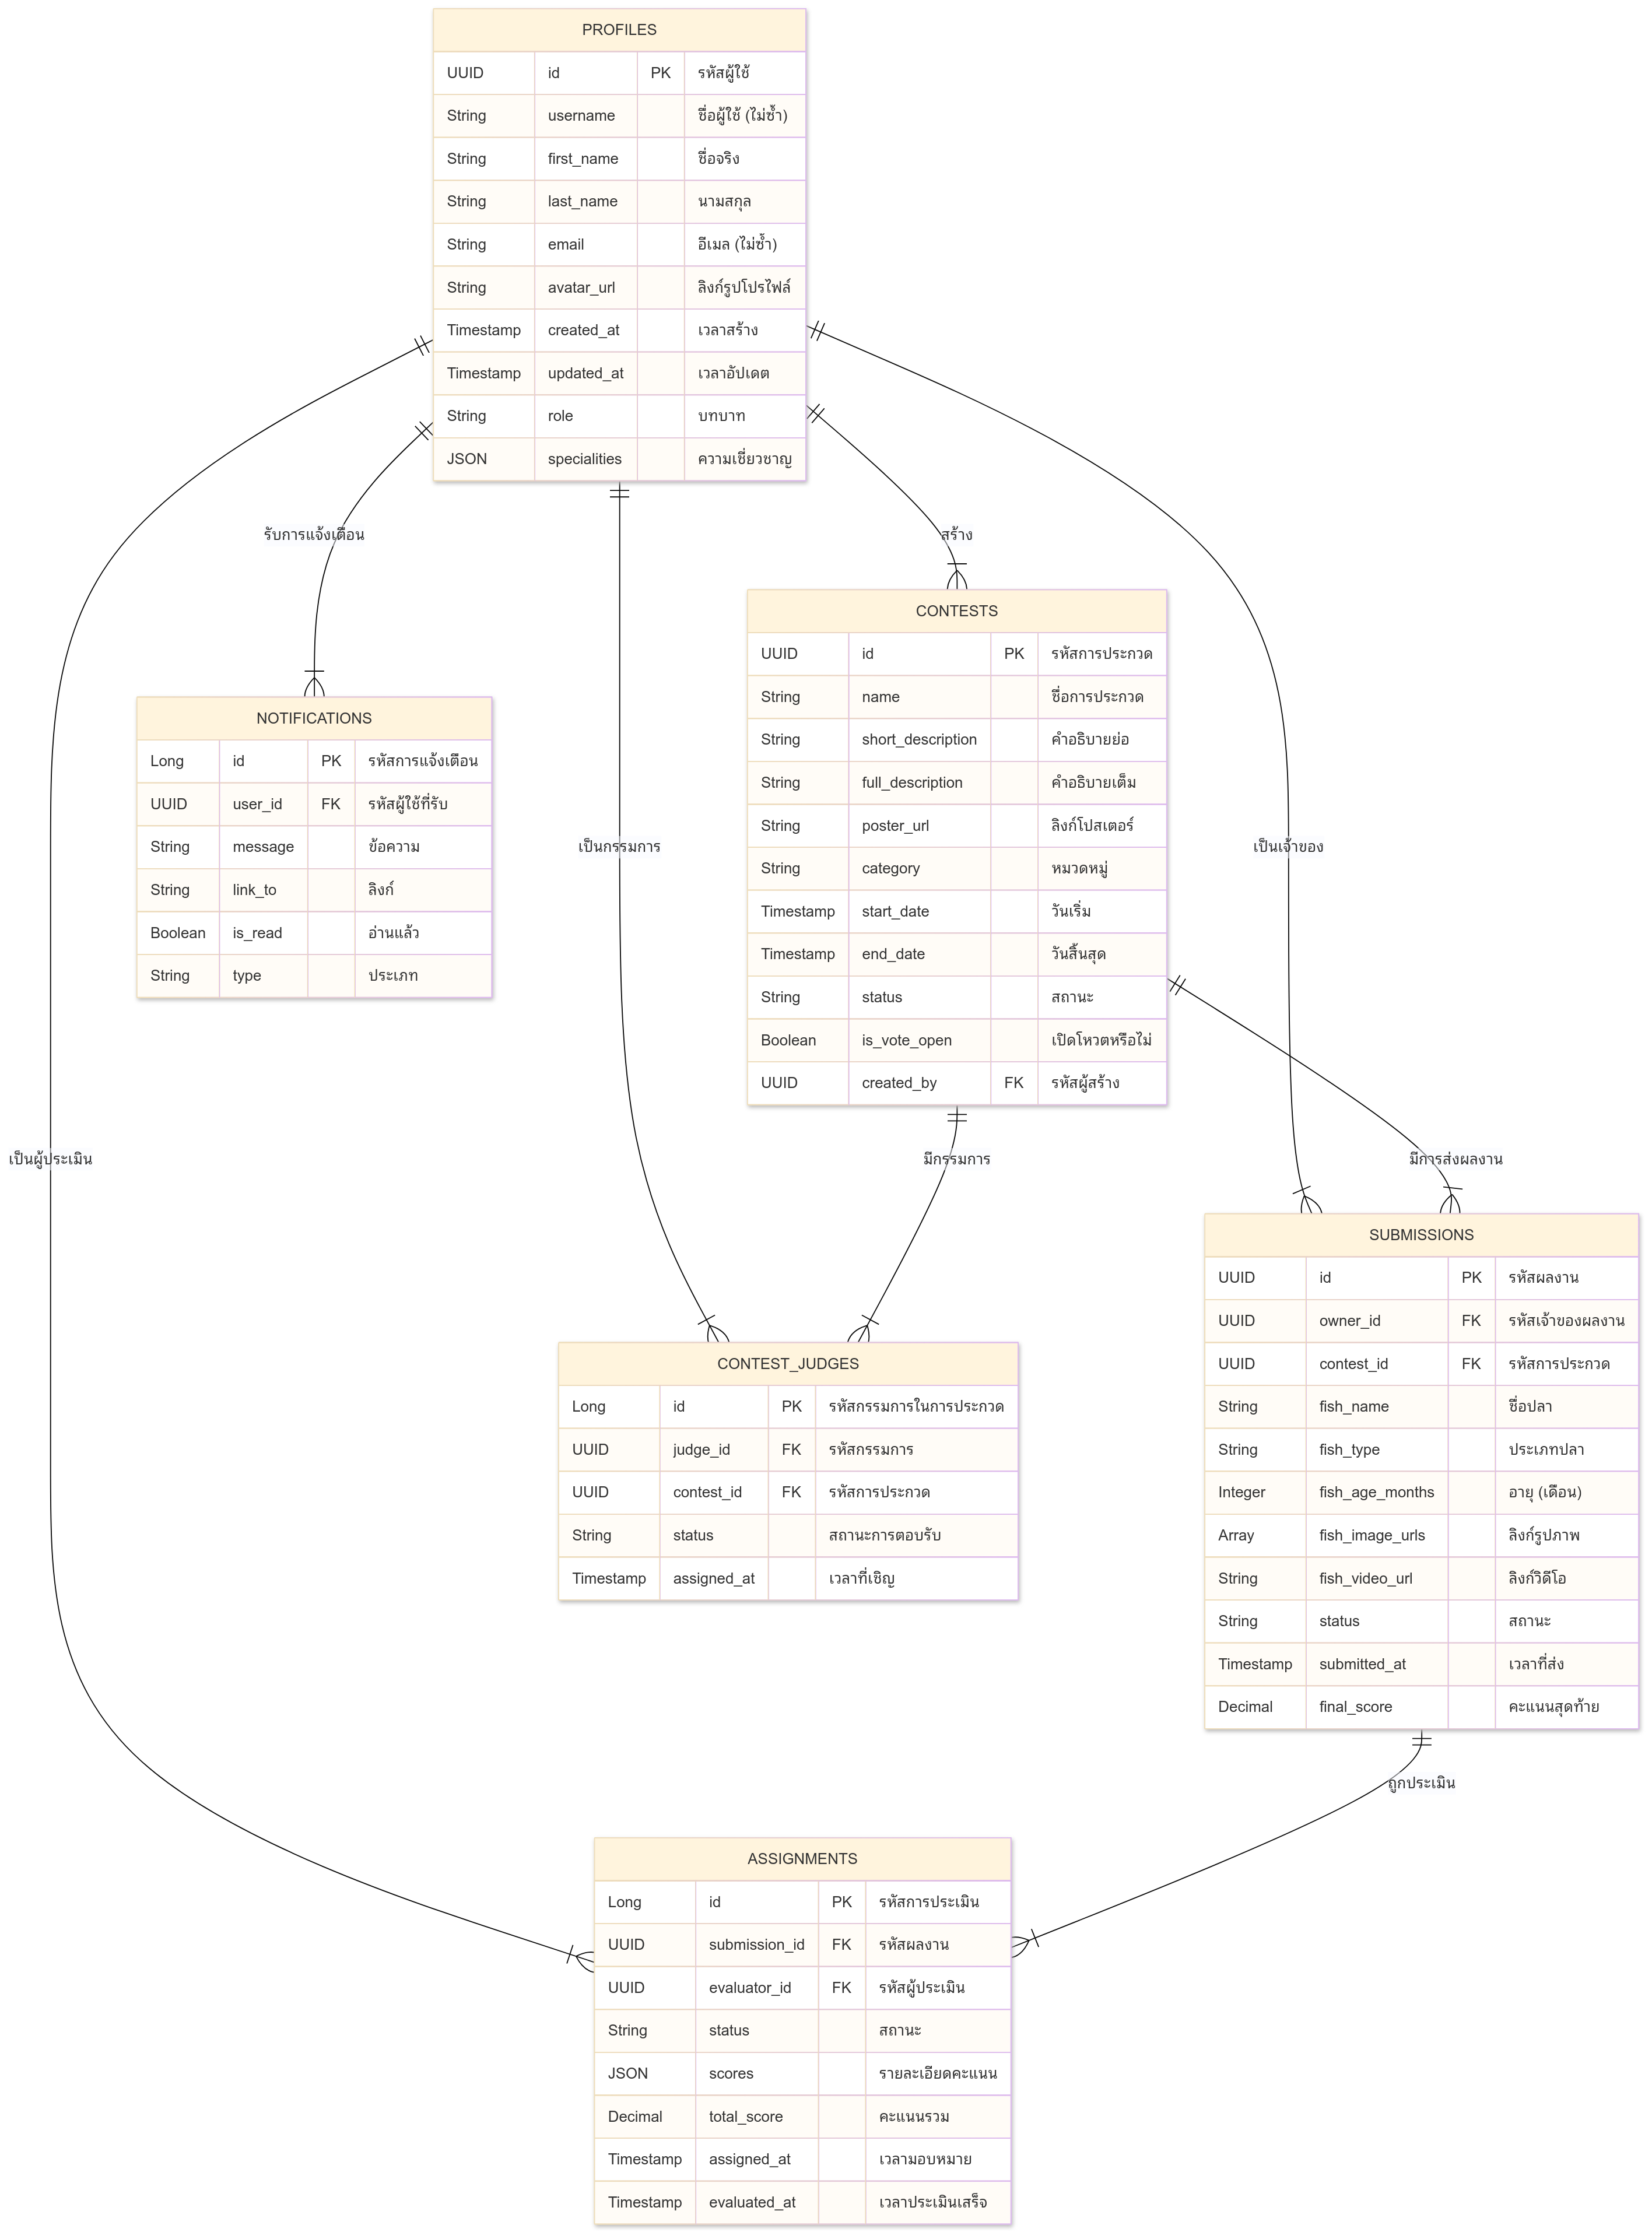
\includegraphics[width=0.8\linewidth]{png2}
	\caption{ENTITY RELATIONSHIP ระบบเว็บแอปพลิเคชันศูนย์รวมการจัดประกวดปลากัดไทย}
\end{figure}

\clearpage}{}
	\IfFileExists{Chapter3_12.tex}{%==================== chapter3_12.tex ====================

\clearpage
\thispagestyle{plain}

\begingroup
\fontsize{16pt}{19.2pt}\selectfont
\justifying
\XeTeXlinebreakskip=0pt plus 1pt minus 0.5pt
\setlength{\parindent}{1.5cm}
\setlength{\parskip}{0pt}

% ตั้งค่าให้เหมือนสเปกเดิมทุกบท
\setlength{\LoneLabelSep}{0.5em}
\settowidth{\LoneLabelWidth}{9.}
\setlength{\LoneContentCol}{\dimexpr 1.5cm + \LoneLabelWidth + \LoneLabelSep\relax}

\setlength{\LtwoLabelSep}{0.5em}
\settowidth{\LtwoLabelWidth}{9.9.}
\setlength{\ExtraAlign}{-2.8em}

% ระดับ 1: อินเดนต์ 1.5 ซม.
\setlist[enumerate,1]{%
	label=\arabic*., align=left,
	leftmargin=1.5cm, labelindent=0pt,
	labelwidth=\LoneLabelWidth, labelsep=\LoneLabelSep,
	itemsep=0pt, topsep=0.5\baselineskip
}

\begin{enumerate}
	\item Entity – Relation Diagram: Profiles
	\item Entity – Relation Diagram: Contests
	\item Entity – Relation Diagram: Submissions
	\item Entity – Relation Diagram: Assignments
	\item Entity – Relation Diagram: ContestJudges
	\item Entity – Relation Diagram: Notifications
\end{enumerate}

\vspace{\baselineskip}

% ---------- หัวข้อใหญ่ (ชิดซ้าย, หนา 16pt) ----------
\noindent{\bfseries\fontsize{16pt}{19.2pt}\selectfont Data Dictionary: เว็บแอปพลิเคชันศูนย์รวมการจัดการประกวดปลากัดไทย}\par


\vspace{\baselineskip}

% ===== Helper for nicer row height (เฉพาะบล็อกนี้) =====
{\renewcommand{\arraystretch}{1.15}
	
	% ========== ER: PROFILES ==========
	\begin{table}[h]
		\caption{Entity -- Relation Diagram: Profiles}
		{\tablefont
			\setlength{\tabcolsep}{6pt}
			\begin{tabularx}{\linewidth}{@{} >{\raggedright\arraybackslash}p{4.2cm} D >{\centering\arraybackslash}p{2.6cm} >{\centering\arraybackslash}p{1.6cm} @{}}
				\Xhline{1.5pt}
				\textbf{Attribute Name} & \textbf{Description} & \textbf{Data Type} & \textbf{Key Type} \\
				\Xhline{0.5pt}
				\textbf{id}        & รหัสเฉพาะสำหรับระบุผู้ใช้งานแต่ละคน & UUID & PK \\
				\Xhline{0.5pt}
				username           & ชื่อแฝงของผู้ใช้สำหรับแสดงผล (ไม่ซ้ำกัน) & String & \\
				\Xhline{0.5pt}
				first\_name        & ชื่อจริงของผู้ใช้ & String & \\
				\Xhline{0.5pt}
				last\_name         & นามสกุลของผู้ใช้ & String & \\
				\Xhline{0.5pt}
				email              & อีเมลสำหรับเข้าระบบและติดต่อ (ไม่ซ้ำกัน) & String & \\
				\Xhline{0.5pt}
				avatar\_url        & ลิงก์รูปภาพโปรไฟล์ของผู้ใช้ & String & \\
				\Xhline{0.5pt}
				created\_at        & วันและเวลาที่สร้างบัญชีผู้ใช้ & Timestamp & \\
				\Xhline{0.5pt}
				updated\_at        & วันและเวลาที่แก้ไขข้อมูลผู้ใช้ล่าสุด & Timestamp & \\
				\Xhline{0.5pt}
				role               & บทบาทของผู้ใช้ในระบบ & String & \\
				\Xhline{0.5pt}
				specialities       & ความเชี่ยวชาญพิเศษ & JSON & \\
				\Xhline{1.5pt}
		\end{tabularx}}
	\end{table}
	

}{}
	\IfFileExists{Chapter3_13.tex}{%==================== chapter3_13.tex ====================

\clearpage
\thispagestyle{plain}

\begingroup
\fontsize{16pt}{19.2pt}\selectfont
\justifying
\XeTeXlinebreakskip=0pt plus 1pt minus 0.5pt
\setlength{\parindent}{1.5cm}
\setlength{\parskip}{0pt}

% ===== Helper for nicer row height (เฉพาะบล็อกนี้) =====
{\renewcommand{\arraystretch}{1.15}
	
	% ========== ER: Contests ==========
	\begin{table}[h]
		\caption{Entity -- Relation Diagram: Contests}
		{\tablefont
			\setlength{\tabcolsep}{6pt}
			\begin{tabularx}{\linewidth}{@{} >{\raggedright\arraybackslash}p{4.2cm} D >{\centering\arraybackslash}p{2.6cm} >{\centering\arraybackslash}p{1.6cm} @{}}
				\Xhline{1.5pt}
				\textbf{Attribute Name} & \textbf{Description} & \textbf{Data Type} & \textbf{Key Type} \\
				\Xhline{0.5pt}
				\textbf{id}            & รหัสการประกวด & UUID & PK \\
				\Xhline{0.5pt}
				name                   & ชื่อการประกวด & String & \\
				\Xhline{0.5pt}
				short\_description      & คำอธิบายย่อ & String & \\
				\Xhline{0.5pt}
				full\_description       & คำอธิบายเต็ม & String & \\
				\Xhline{0.5pt}
				poster\_url             & ลิงก์โปสเตอร์/ภาพประชาสัมพันธ์ & String & \\
				\Xhline{0.5pt}
				category               & หมวดหมู่ & String & \\
				\Xhline{0.5pt}
				start\_date             & วันเริ่ม & Timestamp & \\
				\Xhline{0.5pt}
				end\_date               & วันสิ้นสุด & Timestamp & \\
				\Xhline{0.5pt}
				status                 & สถานะการประกวด (เช่น draft, open, closed) & String & \\
				\Xhline{0.5pt}
				is\_vote\_open           & เปิดโหวตหรือไม่ & Boolean & \\
				\Xhline{0.5pt}
				\textbf{created\_by}    & ผู้สร้างการประกวด & UUID & FK \\
				\Xhline{1.5pt}
			\end{tabularx}}
	\end{table}}{}
	\IfFileExists{Chapter3_14.tex}{%==================== chapter3_14.tex ====================

\clearpage
\thispagestyle{plain}

\begingroup
\fontsize{16pt}{19.2pt}\selectfont
\justifying
\XeTeXlinebreakskip=0pt plus 1pt minus 0.5pt
\setlength{\parindent}{1.5cm}
\setlength{\parskip}{0pt}

% ===== Helper for nicer row height (เฉพาะบล็อกนี้) =====
{\renewcommand{\arraystretch}{1.15}
	
	% ========== ER: SUBMISSIONSsts ==========
	\begin{table}[h]
		\caption{Entity -- Relation Diagram: Submissions}
		{\tablefont
			\setlength{\tabcolsep}{6pt}
			\begin{tabularx}{\linewidth}{@{} >{\raggedright\arraybackslash}p{4.2cm} D >{\centering\arraybackslash}p{2.6cm} >{\centering\arraybackslash}p{1.6cm} @{}}
				\Xhline{1.5pt}
				\textbf{Attribute Name} & \textbf{Description} & \textbf{Data Type} & \textbf{Key Type} \\
				\Xhline{0.5pt}
				\textbf{id}             & รหัสผลงาน & UUID & PK \\
				\Xhline{0.5pt}
				\textbf{owner\_id}       & เจ้าของผลงาน & UUID & FK \\
				\Xhline{0.5pt}
				\textbf{contest\_id}     & อ้างถึงการประกวด & UUID & FK \\
				\Xhline{0.5pt}
				fish\_name               & ชื่อปลา & String & \\
				\Xhline{0.5pt}
				fish\_type               & ประเภทปลา & String & \\
				\Xhline{0.5pt}
				fish\_age\_months         & อายุ (เดือน) & Integer & \\
				\Xhline{0.5pt}
				fish\_image\_urls         & ลิงก์รูปภาพ (หลายรูป) & Array & \\
				\Xhline{0.5pt}
				fish\_video\_url          & ลิงก์วิดีโอ & String & \\
				\Xhline{0.5pt}
				status                  & สถานะผลงาน (เช่น pending, assigned, scored) & String & \\
				\Xhline{0.5pt}
				submitted\_at            & เวลาที่ส่ง & Timestamp & \\
				\Xhline{0.5pt}
				final\_score             & คะแนนสุดท้าย & Decimal & \\
				\Xhline{1.5pt}
			\end{tabularx}}
	\end{table}}{}
	\IfFileExists{Chapter3_15.tex}{%==================== chapter3_15.tex ====================

\clearpage
\thispagestyle{plain}

\begingroup
\fontsize{16pt}{19.2pt}\selectfont
\justifying
\XeTeXlinebreakskip=0pt plus 1pt minus 0.5pt
\setlength{\parindent}{1.5cm}
\setlength{\parskip}{0pt}

% ===== Helper for nicer row height (เฉพาะบล็อกนี้) =====
{\renewcommand{\arraystretch}{1.15}
	
	% ========== ER: ASSIGNMENTS ==========
	\begin{table}[h]
		\caption{Entity -- Relation Diagram: Assignments}
		{\tablefont
			\setlength{\tabcolsep}{6pt}
			\begin{tabularx}{\linewidth}{@{} >{\raggedright\arraybackslash}p{4.2cm} D >{\centering\arraybackslash}p{2.6cm} >{\centering\arraybackslash}p{1.6cm} @{}}
				\Xhline{1.5pt}
				\textbf{Attribute Name} & \textbf{Description} & \textbf{Data Type} & \textbf{Key Type} \\
				\Xhline{0.5pt}
				\textbf{id}             & รหัสการประเมิน & Long & PK \\
				\Xhline{0.5pt}
				\textbf{submission\_id}  & อ้างถึงผลงาน  & UUID & FK \\
				\Xhline{0.5pt}
				\textbf{evaluator\_id}   & ผู้ประเมิน/ผู้เชี่ยวชาญ  & UUID & FK \\
				\Xhline{0.5pt}
				status                  & สถานะ (เช่น assigned, scored) & String & \\
				\Xhline{0.5pt}
				scores                  & รายละเอียดคะแนน (เช่นรายหัวข้อ) & JSON & \\
				\Xhline{0.5pt}
				total\_score             & คะแนนรวม & Decimal & \\
				\Xhline{0.5pt}
				assigned\_at             & เวลามอบหมาย & Timestamp & \\
				\Xhline{0.5pt}
				evaluated\_at            & เวลาประเมินเสร็จ & Timestamp & \\
				\Xhline{1.5pt}
			\end{tabularx}}
	\end{table}
	
\vspace{\baselineskip}
	
	% ========== ER: CONTEST_JUDGES ==========
	\begin{table}[h]
		\caption{Entity -- Relation Diagram: CONTEST\_JUDGES}
		{\tablefont
			\setlength{\tabcolsep}{6pt}
			\begin{tabularx}{\linewidth}{@{} >{\raggedright\arraybackslash}p{4.2cm} D >{\centering\arraybackslash}p{2.6cm} >{\centering\arraybackslash}p{1.6cm} @{}}
				\Xhline{1.5pt}
				\textbf{Attribute Name} & \textbf{Description} & \textbf{Data Type} & \textbf{Key Type} \\
				\Xhline{0.5pt}
				\textbf{id}          & รหัสกรรมการในการประกวด & Long & PK \\
				\Xhline{0.5pt}
				\textbf{judge\_id}    & กรรมการ  & UUID & FK \\
				\Xhline{0.5pt}
				\textbf{contest\_id}  & การประกวด  & UUID & FK \\
				\Xhline{0.5pt}
				status               & สถานะการตอบรับ & String & \\
				\Xhline{0.5pt}
				assigned\_at          & เวลาที่เชิญ & Timestamp & \\
				\Xhline{1.5pt}
			\end{tabularx}}
	\end{table}
\clearpage}{}
	\IfFileExists{Chapter3_16.tex}{%==================== chapter3_16.tex ====================

\clearpage
\thispagestyle{plain}

\begingroup
\fontsize{16pt}{19.2pt}\selectfont
\justifying
\XeTeXlinebreakskip=0pt plus 1pt minus 0.5pt
\setlength{\parindent}{1.5cm}
\setlength{\parskip}{0pt}

% ===== Helper for nicer row height (เฉพาะบล็อกนี้) =====
{\renewcommand{\arraystretch}{1.15}
	
	% ========== ER: NOTIFICATIONS ==========
	\begin{table}[h]
		\caption{Entity -- Relation Diagram: Notifications}
		{\tablefont
			\setlength{\tabcolsep}{6pt}
			\begin{tabularx}{\linewidth}{@{} >{\raggedright\arraybackslash}p{4.2cm} D >{\centering\arraybackslash}p{2.6cm} >{\centering\arraybackslash}p{1.6cm} @{}}
				 \Xhline{1.5pt}
				\textbf{Attribute Name} & \textbf{Description} & \textbf{Data Type} & \textbf{Key Type} \\
				\Xhline{0.5pt}
				\textbf{id}        & รหัสการแจ้งเตือน & Long & PK \\
				\Xhline{0.5pt}
				\textbf{user\_id}   & ผู้ใช้ที่ได้รับ  & UUID & FK \\
				\Xhline{0.5pt}
				message            & ข้อความ & String & \\
				\Xhline{0.5pt}
				link\_to            & ลิงก์ & String & \\
				\Xhline{0.5pt}
				is\_read            & อ่านแล้วหรือไม่ & Boolean & \\
				\Xhline{0.5pt}
				type               & ประเภท & String & \\
				\Xhline{1.5pt}
			\end{tabularx}}
	\end{table}}{}
	\IfFileExists{Chapter3_17.tex}{%==================== chapter3_17.tex ====================

\clearpage
\thispagestyle{plain}

\begingroup
\fontsize{16pt}{19.2pt}\selectfont
\justifying
\XeTeXlinebreakskip=0pt plus 1pt minus 0.5pt
\setlength{\parindent}{1.5cm}
\setlength{\parskip}{0pt}

% ---------- หัวข้อใหญ่ (ชิดซ้าย, หนา 16pt) ----------

\section*{Class Diagram}
\addcontentsline{toc}{section}{Class Diagram}

% ---------- เนื้อหา (จัดกระจายแบบไทย, ย่อหน้าแรก 1.5 ซม.) ----------
\indent Class Diagram: เว็บแอปพลิเคชันศูนย์รวมการจัดการประกวดปลากัดไทย

\vspace{\baselineskip}

\begin{figure}[h]
	\centering
	\includegraphics[width=0.95\linewidth]{ClassDiagram}
	\caption{Class Diagram ระบบเว็บแอปพลิเคชันศูนย์รวมการจัดประกวดปลากัดไทย}
\end{figure}

\clearpage}{}
	\IfFileExists{Chapter3_18.tex}{%==================== chapter3_18.tex ====================

\clearpage
\thispagestyle{plain}

\begingroup
\fontsize{16pt}{19.2pt}\selectfont
\justifying
\XeTeXlinebreakskip=0pt plus 1pt minus 0.5pt
\setlength{\parindent}{1.5cm}
\setlength{\parskip}{0pt}

\vspace{\baselineskip}

% ============================ Class: Profile ============================
\begin{table}[h]
	\caption{Class Description : Profile}
	{\tablefont\setlength{\tabcolsep}{6pt}%
		\begin{tabularx}{\linewidth}{@{} >{\raggedright\arraybackslash}p{3.6cm} X @{}}
			\Xhline{1.5pt}
			\textbf{Class Name :} & Profile \\  % ปิดแถวด้วย \\
			\Xhline{0.5pt}
			\textbf{Description :} & โมเดลผู้ใช้หลักของระบบ ใช้แทนผู้ใช้งานทุกบทบาท และเก็บข้อมูลโปรไฟล์รวมถึงความเชี่ยวชาญ \\
			\Xhline{0.5pt}
			\textbf{Attribute :} &
			\begin{tabular}{@{}l@{}}
				id: UUID — รหัสผู้ใช้ (PK) \\
				username: string — ชื่อผู้ใช้ \\
				first\_name: string — ชื่อ \\
				last\_name: string — นามสกุล \\
				email: string — อีเมล \\
				avatar\_url: string — รูปโปรไฟล์ \\
				created\_at: datetime — เวลาเริ่มสร้าง \\
				updated\_at: datetime — เวลาอัปเดต \\
				role: string — บทบาท \\
				specialities: JSON — ความเชี่ยวชาญของผู้เชี่ยวชาญ
			\end{tabular} \\
			\Xhline{0.5pt}
			\textbf{Method :} &
			\begin{tabular}{@{}l@{}}
				fetchProfile(): ดึงโปรไฟล์ผู้ใช้ปัจจุบัน \\
				updateProfile(profileData): อัปเดตข้อมูลโปรไฟล์ \\
				uploadProfilePicture(file): อัปโหลดรูปโปรไฟล์
			\end{tabular} \\
			\Xhline{1.5pt}
	\end{tabularx}}
\end{table}

\newpage

% ============================ Class: Contest ============================
\begin{table}[h]
	\caption{Class Description : Contest}
	{\tablefont\setlength{\tabcolsep}{6pt}%
		\begin{tabularx}{\linewidth}{@{} >{\raggedright\arraybackslash}p{3.6cm} X @{}}
			\Xhline{1.5pt}
			\textbf{Class Name :} & Contest \\ 
			\Xhline{0.5pt}
			\textbf{Description :} & กิจกรรมการประกวด/ข่าวสารที่จัดโดยผู้จัดการการแข่งขัน ใช้ควบคุมสถานะและช่วงเวลา \\
			\Xhline{0.5pt}
			\textbf{Attribute :} &
			\begin{tabular}{@{}l@{}}
				id: UUID — รหัสการประกวด (PK) \\
				name: string — ชื่อการประกวด \\
				short\_description: string — คำอธิบายสั้น \\
				full\_description: string — คำอธิบายเต็ม \\
				poster\_url: string — โปสเตอร์ \\
				category: string — หมวดหมู่ \\
				start\_date: datetime — วันเริ่ม \\
				end\_date: datetime — วันจบ \\
				status: string — สถานะ \\
				is\_vote\_open: boolean — เปิดโหวตหรือไม่ \\
				created\_by: UUID — ผู้สร้าง (Profile.id)
			\end{tabular} \\
			\Xhline{0.5pt}
			\textbf{Method :} &
			\begin{tabular}{@{}l@{}}
				createContestOrNews(formData): สร้างกิจกรรม/ข่าว \\
				getMyContests(): ดึงรายการกิจกรรมของผู้จัดการ \\
				getContestDetail(contestId, isContest): ดึงรายละเอียดกิจกรรม \\
				updateMyContest(contestId, data): อัปเดตกิจกรรม \\
				deleteMyContest(contestId): ลบกิจกรรม \\
				updateContestStatus(contestId, status): เปลี่ยนสถานะ \\
				finalizeContest(contestId): ปิดและประกาศผล \\
				getContestSubmissions(contestId): ดึงรายการผู้สมัคร \\
				getScoringProgress(contestId): ความคืบหน้าการให้คะแนน \\
				getAllResults(): ดึงสรุปผลคะแนนทั้งหมด
			\end{tabular} \\
			\Xhline{1.5pt}
	\end{tabularx}}
\end{table}

\newpage

% ============================ Class: Submission ============================
\begin{table}[h]
	\caption{Class Description : Submission}
	{\tablefont\setlength{\tabcolsep}{6pt}%
		\begin{tabularx}{\linewidth}{@{} >{\raggedright\arraybackslash}p{3.6cm} X @{}}
			\Xhline{1.5pt}
			\textbf{Class Name :} & Submission \\
			\Xhline{0.5pt}
			\textbf{Description :} & การส่งผลงานปลากัดของผู้ใช้ ทั้งเพื่อการประเมินคุณภาพและเพื่อเข้าร่วมประกวด \\
			\Xhline{0.5pt}
			\textbf{Attribute :} &
			\begin{tabular}{@{}l@{}}
				id: UUID — รหัสการส่ง (PK) \\
				owner\_id: UUID — เจ้าของ (Profile.id) \\
				contest\_id: UUID — การประกวดที่เข้าร่วม (nullable เมื่อประเมินคุณภาพ) \\
				fish\_name: string — ชื่อปลา \\
				fish\_type: string — ประเภท/สายพันธุ์ \\
				fish\_age\_months: int — อายุ (เดือน) \\
				fish\_image\_urls: string[] — ลิงก์รูป \\
				fish\_video\_url: string — ลิงก์วิดีโอ \\
				status: string — สถานะ \\
				submitted\_at: datetime — เวลาส่ง \\
				final\_score: decimal — คะแนนสุดท้าย (ถ้ามี)
			\end{tabular} \\
			\Xhline{0.5pt}
			\textbf{Method :} &
			\begin{tabular}{@{}l@{}}
				submitBettaForEvaluation(formData): ส่งประเมินคุณภาพ \\
				submitBettaForCompetition(formData): ส่งเข้าประกวด \\
				getScoresForSubmission(submissionId): ดึงคะแนนของผลงาน
			\end{tabular} \\
			\Xhline{1.5pt}
	\end{tabularx}}
\end{table}

\clearpage}{}
	\IfFileExists{Chapter3_19.tex}{%==================== chapter3_19.tex ====================

\clearpage
\thispagestyle{plain}

\begingroup
\fontsize{16pt}{19.2pt}\selectfont
\justifying
\XeTeXlinebreakskip=0pt plus 1pt minus 0.5pt
\setlength{\parindent}{1.5cm}
\setlength{\parskip}{0pt}

\vspace{\baselineskip}


% ============================ Class: ContestJudge ============================
\begin{table}[h]
	\caption{Class Description : ContestJudge}
	{\tablefont\setlength{\tabcolsep}{6pt}%
		\begin{tabularx}{\linewidth}{@{} >{\raggedright\arraybackslash}p{3.6cm} X @{}}
			\Xhline{1.5pt}
			\textbf{Class Name :} & ContestJudge \\
			\Xhline{0.5pt}
			\textbf{Description :} & การเป็นกรรมการของผู้เชี่ยวชาญในกิจกรรมการประกวด รวมถึงสถานะคำเชิญ \\
			\Xhline{0.5pt}
			\textbf{Attribute :} &
			\begin{tabular}{@{}l@{}}
				id: long — รหัสแถว (PK) \\
				judge\_id: UUID — ผู้เชี่ยวชาญ (Profile.id) \\
				contest\_id: UUID — การประกวด \\
				status: string — สถานะคำเชิญ/บทบาท (invited, accepted, declined ฯลฯ) \\
				assigned\_at: datetime — เวลามอบหมาย
			\end{tabular} \\
			\Xhline{0.5pt}
			\textbf{Method :} &
			\begin{tabular}{@{}l@{}}
				getJudgingContests(): ดึงรายการประกวดที่เกี่ยวข้อง \\
				respondToJudgeInvitation(contestId, response, reason): ตอบรับ/ปฏิเสธ \\
				assignJudgeToContest(contestId, judgeId): มอบหมายกรรมการ \\
				removeJudgeFromContest(contestId, judgeId): ถอดกรรมการ \\
				notifyJudgeRemoval(contestId, judgeId, options): แจ้งเตือนการถอด
			\end{tabular} \\
			\Xhline{1.5pt}
	\end{tabularx}}
\end{table}

%\newpage

% ============================ Class: Assignment ============================
\begin{table}[h]
	\caption{Class Description : Assignment}
	{\tablefont\setlength{\tabcolsep}{6pt}%
		\begin{tabularx}{\linewidth}{@{} >{\raggedright\arraybackslash}p{3.6cm} X @{}}
			\Xhline{1.5pt}
			\textbf{Class Name :} & Assignment \\
			\Xhline{0.5pt}
			\textbf{Description :} & งานที่มอบหมายให้ผู้เชี่ยวชาญประเมินผลงาน เก็บคะแนนย่อยและผลรวม \\
			\Xhline{0.5pt}
			\textbf{Attribute :} &
			\begin{tabular}{@{}l@{}}
				id: long — รหัสงาน (PK) \\
				submission\_id: UUID — อ้างอิงผลงาน \\
				evaluator\_id: UUID — ผู้ประเมิน (Profile.id) \\
				status: string — สถานะงาน (queued, accepted, rejected, evaluated ฯลฯ) \\
				scores: JSON — รายละเอียดคะแนน \\
				total\_score: decimal — คะแนนรวม \\
				assigned\_at: datetime — เวลาได้รับมอบหมาย \\
				evaluated\_at: datetime — เวลาประเมินเสร็จ
			\end{tabular} \\
			\Xhline{0.5pt}
			\textbf{Method :} &
			\begin{tabular}{@{}l@{}}
				getEvaluationQueue(): ดึงคิวงานประเมินของผู้เชี่ยวชาญ \\
				respondToEvaluation(assignmentId, status, reason): ตอบรับ/ปฏิเสธงาน \\
				submitQualityScores(assignmentId, scoresData): ส่งคะแนนโหมดคุณภาพ \\
				getScoringSchema(bettaType, options): ดึงเกณฑ์การให้คะแนนแบบไดนามิก
			\end{tabular} \\
			\Xhline{1.5pt}
	\end{tabularx}}
\end{table}

\newpage

% ============================ Class: Notification ============================
\begin{table}[h]
	\caption{Class Description : Notification}
	{\tablefont\setlength{\tabcolsep}{6pt}%
		\begin{tabularx}{\linewidth}{@{} >{\raggedright\arraybackslash}p{3.6cm} X @{}}
			\Xhline{1.5pt}
			\textbf{Class Name :} & Notification \\
			\Xhline{0.5pt}
			\textbf{Description :} & การแจ้งเตือนของระบบที่ส่งถึงผู้ใช้แต่ละคน ใช้แจ้งผลการประกวด การมอบหมาย หรือการเปลี่ยนสถานะ \\
			\Xhline{0.5pt}
			\textbf{Attribute :} &
			\begin{tabular}{@{}l@{}}
				id: long — รหัสแจ้งเตือน (PK) \\
				user\_id: UUID — ผู้รับ \\
				message: string — ข้อความ \\
				link\_to: string — ลิงก์ไปยังหน้าที่เกี่ยวข้อง \\
				is\_read: boolean — อ่านแล้วหรือยัง \\
				type: string — ประเภทแจ้งเตือน \\
				created\_at: datetime — เวลาแจ้งเตือน
			\end{tabular} \\
			\Xhline{0.5pt}
			\textbf{Method :} &
			\begin{tabular}{@{}l@{}}
				getMyNotifications(opts): ดึงรายการแจ้งเตือนของผู้ใช้ \\
				markNotificationRead(id): ทำรายการเดียวเป็นอ่านแล้ว \\
				markAllNotificationsRead(): ทำทั้งหมดเป็นอ่านแล้ว \\
				countUnread(): นับจำนวนที่ยังไม่อ่าน
			\end{tabular} \\
			\Xhline{1.5pt}
	\end{tabularx}}
\end{table}

\clearpage}{}
	\IfFileExists{Chapter3_20.tex}{%==================== chapter3_20.tex ====================

\clearpage
\thispagestyle{plain}

\begingroup
\fontsize{16pt}{19.2pt}\selectfont
\justifying
\XeTeXlinebreakskip=0pt plus 1pt minus 0.5pt
\setlength{\parindent}{1.5cm}
\setlength{\parskip}{0pt}

\vspace{\baselineskip}

% ========================= Class: SubmissionController ==========================
\begin{table}[h]
	\caption{Class Description : SubmissionController}
	{\tablefont\setlength{\tabcolsep}{6pt}%
		\begin{tabularx}{\linewidth}{@{} >{\raggedright\arraybackslash}p{3.6cm} D @{}}
			\Xhline{1.5pt}
			\textbf{Class Name :} & SubmissionController \\
			\Xhline{0.5pt}
			\textbf{Description :} & Controller จุดรับ Endpoint สำหรับการส่งปลากัดเข้าระบบ ทั้งแบบประเมินคุณภาพและแบบเข้าร่วมการแข่งขัน \\
			\Xhline{0.5pt}
			\textbf{Attribute :} & - \\
			\Xhline{0.5pt}
			\textbf{Method :} &
			\begin{tabular}{@{}l@{}}
				createEvaluationSubmission(req, res): ส่งปลากัดเพื่อประเมินคุณภาพ \\
				createCompetitionSubmission(req, res): ส่งปลากัดเพื่อเข้าร่วมการแข่งขัน
			\end{tabular} \\
			\Xhline{1.5pt}
	\end{tabularx}}
\end{table}

% ============================== Class: SubmissionService =======================
\begin{table}[h]
	\caption{Class Description : SubmissionService}
	{\tablefont\setlength{\tabcolsep}{6pt}%
		\begin{tabularx}{\linewidth}{@{} >{\raggedright\arraybackslash}p{3.6cm} D @{}}
			\Xhline{1.5pt}
			\textbf{Class Name :} & SubmissionService \\
			\Xhline{0.5pt}
			\textbf{Description :} & Service จัดการ Logic การสร้าง Submission ลงในฐานข้อมูล ทำหน้าที่เป็นตัวกลางก่อนมอบหมายงานต่อไป \\
			\Xhline{0.5pt}
			\textbf{Attribute :} & - \\
			\Xhline{0.5pt}
			\textbf{Method :} &
			\begin{tabular}{@{}l@{}}
				createSubmission(params): สร้างข้อมูล Submission ใหม่ในตาราง submissions
			\end{tabular} \\
			\Xhline{1.5pt}
	\end{tabularx}}
\end{table}

% ============================== Class: ModelApiService =========================
\begin{table}[h]
	\caption{Class Description : ModelApiService}
	{\tablefont\setlength{\tabcolsep}{6pt}%
		\begin{tabularx}{\linewidth}{@{} >{\raggedright\arraybackslash}p{3.6cm} D @{}}
			\Xhline{1.5pt}
			\textbf{Class Name :} & ModelApiService \\
			\Xhline{0.5pt}
			\textbf{Description :} & Service สำหรับเชื่อมต่อกับ External AI Model (Hugging Face) เพื่อวิเคราะห์ประเภทปลากัดจากรูปภาพที่ผู้ใช้อัปโหลด \\
			\Xhline{0.5pt}
			\textbf{Attribute :} & - \\
			\Xhline{0.5pt}
			\textbf{Method :} &
			\begin{tabular}{@{}l@{}}
				predictBettaType(imageBuffer): ส่งรูปภาพ (Buffer) ไปยัง Model API และรับผลการ\\วิเคราะห์
			\end{tabular} \\
			\Xhline{1.5pt}
	\end{tabularx}}
\end{table}}{}
	\IfFileExists{Chapter3_21.tex}{%==================== chapter3_21.tex ====================

\clearpage
\thispagestyle{plain}

\begingroup
\fontsize{16pt}{19.2pt}\selectfont
\justifying
\XeTeXlinebreakskip=0pt plus 1pt minus 0.5pt
\setlength{\parindent}{1.5cm}
\setlength{\parskip}{0pt}

\vspace{\baselineskip}

% ================================= Class: SupabaseAdmin ========================
\begin{table}[h]
	\caption{Class Description : SupabaseAdmin}
	{\tablefont\setlength{\tabcolsep}{6pt}%
		\begin{tabularx}{\linewidth}{@{} >{\raggedright\arraybackslash}p{3.6cm} D @{}}
			\Xhline{1.5pt}
			\textbf{Class Name :} & SupabaseAdmin \\
			\Xhline{0.5pt}
			\textbf{Description :} & Client กลางสำหรับติดต่อกับ Supabase โดยใช้ SERVICE\_ROLE\_KEY ข้ามกฎ RLS เพื่อจัดการข้อมูลระดับ Admin \\
			\Xhline{0.5pt}
			\textbf{Attribute :} & - \\
			\Xhline{0.5pt}
			\textbf{Method :} &
			\begin{tabular}{@{}l@{}}
				rpc(function, params): เรียกใช้ Database Function \\
				from(table): เลือกตารางเพื่อดำเนินการ (CRUD) \\
				storage(): เข้าถึงส่วนจัดการไฟล์ (Storage)
			\end{tabular} \\
			\Xhline{1.5pt}
	\end{tabularx}}
\end{table}

% ============================= Class: NotificationService ======================
\begin{table}[h]
	\caption{Class Description : NotificationService}
	{\tablefont\setlength{\tabcolsep}{6pt}%
		\begin{tabularx}{\linewidth}{@{} >{\raggedright\arraybackslash}p{3.6cm} D @{}}
			\Xhline{1.5pt}
			\textbf{Class Name :} & NotificationService \\
			\Xhline{0.5pt}
			\textbf{Description :} & Service กลางสำหรับสร้างและจัดการการแจ้งเตือน (Notifications) ไปยังผู้ใช้ในเหตุการณ์ต่าง ๆ \\
			\Xhline{0.5pt}
			\textbf{Attribute :} & - \\
			\Xhline{0.5pt}
			\textbf{Method :} &
			\begin{tabular}{@{}l@{}}
				createNotification(userId, message): สร้างการแจ้งเตือนใหม่สำหรับผู้ใช้ที่ระบุ
			\end{tabular} \\
			\Xhline{1.5pt}
	\end{tabularx}}
\end{table}

% =================================== Class: ApiService =========================
\begin{table}[h]
	\caption{Class Description : ApiService}
	{\tablefont\setlength{\tabcolsep}{6pt}%
		\begin{tabularx}{\linewidth}{@{} >{\raggedright\arraybackslash}p{3.6cm} D @{}}
			\Xhline{1.5pt}
			\textbf{Class Name :} & ApiService \\
			\Xhline{0.5pt}
			\textbf{Description :} & Service กลางของ Frontend ทำหน้าที่เป็น Wrapper ของ \texttt{fetch} API เพื่อสื่อสารกับ Backend ทั้งหมด จัดการ Token, Headers และ Error เบื้องต้น \\
			\Xhline{0.5pt}
			\textbf{Attribute :} & - \\
			\Xhline{0.5pt}
			\textbf{Method :} &
			\begin{tabular}{@{}l@{}}
			get(endpoint): ส่ง GET request \\
			post(endpoint, body): ส่ง POST request \\
			put(endpoint, body): ส่ง PUT request \\
			delete(endpoint): ส่ง DELETE request
			\end{tabular} \\
			\Xhline{1.5pt}
	\end{tabularx}}
\end{table}}{}
	\IfFileExists{Chapter3_22.tex}{%==================== chapter3_22.tex ====================

\clearpage
\thispagestyle{plain}

\begingroup
\fontsize{16pt}{19.2pt}\selectfont
\justifying
\XeTeXlinebreakskip=0pt plus 1pt minus 0.5pt
\setlength{\parindent}{1.5cm}
\setlength{\parskip}{0pt}

\vspace{\baselineskip}

% =============================== Class: [Role]ServiceFE ========================
\begin{table}[h]
	\caption{Class Description : [Role]ServiceFE (เช่น ManagerServiceFE, ExpertServiceFE)}
	{\tablefont\setlength{\tabcolsep}{6pt}%
		\begin{tabularx}{\linewidth}{@{} >{\raggedright\arraybackslash}p{3.6cm} D @{}}
			\Xhline{1.5pt}
			\textbf{Class Name :} & [Role]ServiceFE \\
			\Xhline{0.5pt}
			\textbf{Description :} & กลุ่ม Service ฝั่ง Frontend แยก Logic การเรียกใช้ API ตามบทบาทผู้ใช้ เพื่อให้ Component ไม่เรียก ApiService โดยตรง \\
			\Xhline{0.5pt}
			\textbf{Attribute :} & - \\
			\Xhline{0.5pt}
			\textbf{Method :} &
			\begin{tabular}{@{}l@{}}
				getMyContests(): เรียก ApiService.get ไปยัง endpoint ของ Manager \\
				getEvaluationQueue(): เรียก ApiService.get ไปยัง endpoint ของ Expert
			\end{tabular} \\
			\Xhline{1.5pt}
	\end{tabularx}}
\end{table}

% ============================ Class: [Page/Component] ==========================
\begin{table}[h]
	\caption{Class Description : [Page/Component] (เช่น LiveContestRoom, EvaluationQueue)}
	{\tablefont\setlength{\tabcolsep}{6pt}%
		\begin{tabularx}{\linewidth}{@{} >{\raggedright\arraybackslash}p{3.6cm} D @{}}
			\Xhline{1.5pt}
			\textbf{Class Name :} & [Page/Component] \\
			\Xhline{0.5pt}
			\textbf{Description :} & Component แสดงผล UI สำหรับบทบาทต่าง ๆ โดยเรียกใช้ Service (FE) ที่เกี่ยวข้องเพื่อนำข้อมูลมาแสดงและส่งกลับ Backend \\
			\Xhline{0.5pt}
			\textbf{Attribute :} &
			\begin{tabular}{@{}l@{}}
				selectedContest / queue: state สำหรับเก็บข้อมูลที่ดึงมา
			\end{tabular} \\
			\Xhline{0.5pt}
			\textbf{Method :} &
			\begin{tabular}{@{}l@{}}
				handle...(): ฟังก์ชันจัดการเหตุการณ์จากผู้ใช้ (เช่น คลิก) และเรียกใช้ Service
			\end{tabular} \\
			\Xhline{1.5pt}
	\end{tabularx}}
\end{table}

% ============================= Class: SubmissionFormModal ======================
\begin{table}[h]
	\caption{Class Description : SubmissionFormModal}
	{\tablefont\setlength{\tabcolsep}{6pt}%
		\begin{tabularx}{\linewidth}{@{} >{\raggedright\arraybackslash}p{3.6cm} D @{}}
			\Xhline{1.5pt}
			\textbf{Class Name :} & SubmissionFormModal \\
			\Xhline{0.5pt}
			\textbf{Description :} & Modal สำหรับรับข้อมูลการส่งปลากัดจากผู้ใช้ จัดการ state ของรูปภาพ วิดีโอ และข้อมูลในฟอร์ม \\
			\Xhline{0.5pt}
			\textbf{Attribute :} &
			\begin{tabular}{@{}l@{}}
				images: state สำหรับเก็บไฟล์รูปภาพ \\
				video: state สำหรับเก็บไฟล์วิดีโอ
			\end{tabular} \\
			\Xhline{0.5pt}
			\textbf{Method :} &
			\begin{tabular}{@{}l@{}}
				onSubmit(): เรียกใช้เมื่อผู้ใช้ยืนยันการส่งข้อมูล โดยจะเรียก UserServiceFE \\และ ModelServiceFE
			\end{tabular} \\
			\Xhline{1.5pt}
	\end{tabularx}}
\end{table}
}{}
	\IfFileExists{Chapter3_23.tex}{%==================== chapter3_23.tex ====================

\clearpage
\thispagestyle{plain}

\begingroup
\fontsize{16pt}{19.2pt}\selectfont
\justifying
\XeTeXlinebreakskip=0pt plus 1pt minus 0.5pt
\setlength{\parindent}{1.5cm}
\setlength{\parskip}{0pt}

\vspace{\baselineskip}

% =================================== Class: AuthContext ========================
\begin{table}[h]
	\caption{Class Description : AuthContext}
	{\tablefont\setlength{\tabcolsep}{6pt}%
		\begin{tabularx}{\linewidth}{@{} >{\raggedright\arraybackslash}p{3.6cm} D @{}}
			\Xhline{1.5pt}
			\textbf{Class Name :} & AuthContext \\
			\Xhline{0.5pt}
			\textbf{Description :} & React Context สำหรับ Global State การยืนยันตัวตน เก็บ user, isAuthenticated และฟังก์ชัน signin/signout \\
			\Xhline{0.5pt}
			\textbf{Attribute :} &
			\begin{tabular}{@{}l@{}}
				user: ข้อมูลโปรไฟล์ผู้ใช้ปัจจุบัน \\
				isAuthenticated: สถานะล็อกอิน (boolean)
			\end{tabular} \\
			\Xhline{0.5pt}
			\textbf{Method :} &
			\begin{tabular}{@{}l@{}}
				signin(): เข้าสู่ระบบ \\
				signout(): ออกจากระบบ
			\end{tabular} \\
			\Xhline{1.5pt}
	\end{tabularx}}
\end{table}

% ================================== Class: ProtectedRoute ======================
\begin{table}[h]
	\caption{Class Description : ProtectedRoute}
	{\tablefont\setlength{\tabcolsep}{6pt}%
		\begin{tabularx}{\linewidth}{@{} >{\raggedright\arraybackslash}p{3.6cm} D @{}}
			\Xhline{1.5pt}
			\textbf{Class Name :} & ProtectedRoute \\
			\Xhline{0.5pt}
			\textbf{Description :} & Higher-Order Component ทำหน้าที่ตรวจสอบสิทธิ์จาก AuthContext ก่อนอนุญาตให้เข้าถึงแต่ละ Route \\
			\Xhline{0.5pt}
			\textbf{Attribute :} &
			\begin{tabular}{@{}l@{}}
				requiredRole: บทบาทที่จำเป็นสำหรับการเข้าถึงหน้า
			\end{tabular} \\
			\Xhline{0.5pt}
			\textbf{Method :} & - \\
			\Xhline{1.5pt}
	\end{tabularx}}
\end{table}}{}
	\IfFileExists{Chapter3_24.tex}{%==================== chapter3_24.tex ====================

\clearpage
\thispagestyle{plain}

\begingroup
\fontsize{16pt}{19.2pt}\selectfont
\justifying
\XeTeXlinebreakskip=0pt plus 1pt minus 0.5pt
\setlength{\parindent}{1.5cm}
\setlength{\parskip}{0pt}

% ---------- หัวข้อใหญ่ (ชิดซ้าย, หนา 16pt) ----------
\section*{Sequence Diagra}
\addcontentsline{toc}{section}{Sequence Diagra}

% ---------- เนื้อหา (จัดกระจายแบบไทย, ย่อหน้าแรก 1.5 ซม.) ----------
\indent Sequence Diagram เป็นแผนผังแสดงการทำงานแบบลำดับปฏิสัมพันธ์ โดยเว็บแอปพลิเคชันศูนย์รวมการจัดประกวดปลากัดไทย มีองค์ประกอบ Sequence Diagram ดังนี้

% ===== enumerate แบบ robust (ไม่ใช้ \dimexpr เพื่อกัน error) =====
\setlist[enumerate,1]{%
	label=\arabic*., align=left,
	leftmargin=1.5cm, labelindent=0pt,
	labelwidth=\LoneLabelWidth, labelsep=\LoneLabelSep,
	itemsep=0pt, topsep=0.5\baselineskip
}

% ระดับ 2: ให้คอลัมน์ข้อความตรงตามที่ตั้ง (ชิฟต์ด้วย \ExtraAlign)
\setlist[enumerate,2]{%
	label*=\arabic*., align=left,
	leftmargin=*,
	labelwidth=\LtwoLabelWidth, labelsep=\LtwoLabelSep,
	labelindent=\dimexpr \LoneContentCol + \ExtraAlign - \LtwoLabelWidth - \LtwoLabelSep\relax,
	itemsep=0pt, topsep=0pt
}
\setlist[enumerate,3]{%
	label*=\arabic*., align=left,
	leftmargin=*, labelsep=-0.6em,
	labelindent=-1em, % ให้คอลัมน์ข้อความตรงเส้นเดียวกับระดับ 2
	widest=9.9.9,
	itemsep=0pt, topsep=0pt
}

\begin{enumerate}
	\item การเข้าสู่ระบบ
	\item การสมัครสมาชิก
	\item การออกจากระบบ
	\item การกู้คืนเซสชันเมื่อเข้าแอป
	\item การอัปเดตโปรไฟล์ผู้ใช้
	\item การอัปโหลดรูปโปรไฟล์
	\item ผู้ใช้ส่งปลากัดเพื่อประเมินคุณภาพ
	\item ผู้ใช้ส่งปลากัดเข้าร่วมการแข่งขัน
	\item ผู้เชี่ยวชาญดึงคิวงานประเมินคุณภาพ
	\item ผู้เชี่ยวชาญตอบรับ/ปฏิเสธงานประเมิน
	\item ผู้เชี่ยวชาญส่งคะแนนประเมินคุณภาพ
	\item ดึงเกณฑ์การให้คะแนนตามประเภทปลา
	\item ผู้เชี่ยวชาญดูรายการประกวดที่ต้องตัดสิน (มีฟอลแบ็ก)
	\item ผู้เชี่ยวชาญตอบรับ/ปฏิเสธคำเชิญเป็นกรรมการ
	\item ดึงรายชื่อปลาที่เข้าประกวดในกิจกรรม
	\item ผู้เชี่ยวชาญส่งคะแนนการแข่งขัน
	\item ผู้จัดการสร้างกิจกรรม/ข่าว
	\item ผู้จัดการแก้ไขกิจกรรม
	\item ผู้จัดการมอบหมาย/ถอดถอนกรรมการและส่งแจ้งเตือน
	\item ผู้จัดการปิดการแข่งขันและประกาศผล
	\item ผู้ใช้เปิดศูนย์แจ้งเตือนและทำเครื่องหมายอ่านทั้งหมด
	\item วิเคราะห์รูปภาพด้วย AI สำหรับการแข่งขัน (เดี่ยว/หลายรูป)
	\item ผู้ใช้ดูผลการแข่งขันแบบสาธารณะ
	\item ประวัติการทำงานของผู้เชี่ยวชาญ (สลับแท็บ คุณภาพ/การแข่งขัน)
	\item ประวัติการส่งของผู้ใช้ (คุณภาพ/การแข่งขัน)
\end{enumerate}

\vspace{\baselineskip}

\begin{figure}[h]
	\centering
	\includegraphics[width=0.8\linewidth]{SQ1}
	\caption{การเข้าสู่ระบบ}
\end{figure}

\indent ไดอะแกรมนี้แสดงลำดับเหตุการณ์เมื่อผู้ใช้พยายามเข้าสู่ระบบ หน้า Login รับอินพุตจากผู้ใช้และตรวจสอบความครบถ้วน จากนั้นเรียก AuthContext.signin ซึ่งภายในจะเด้งไปเรียก authService.loginUser เพื่อยิง POST /auth/signin ผ่าน apiService ไปยัง Backend เมื่อสำเร็จเซิร์ฟเวอร์ส่ง token และ profile กลับมา ฝั่งฟรอนต์จะบันทึกลง localStorage แล้วอัปเดตสเตต user ใน AuthContext จากนั้นหน้า Login แสดง Toast สำเร็จและเปลี่ยนเส้นทางตาม role ของผู้ใช้ หากล้มเหลว หน้า Login แสดงข้อความผิดพลาดโดยไม่เปลี่ยนเส้นทาง

\newpage

\begin{figure}[h]
	\centering
	\includegraphics[width=0.8\linewidth]{SQ2}
	\caption{การสมัครสมาชิก}
\end{figure}

\indent แผนภาพนี้อธิบายการสร้างบัญชีผู้ใช้ใหม่ หน้า SignUp ตรวจความครบถ้วนของข้อมูลก่อนเรียก authService.signupUser ซึ่งยิง POST /auth/signup ผ่าน apiService ไปยัง Backend เมื่อสำเร็จจะตอบ 201 Created กลับมา หน้า SignUp แสดง Toast สำเร็จและนำผู้ใช้ไปหน้า Login ในกรณีผิดพลาด หน้า SignUp แสดงสาเหตุข้อผิดพลาดเพื่อให้แก้ไขข้อมูลและลองใหม่


\newpage

\vspace{\baselineskip}

\begin{figure}[h]
	\centering
	\includegraphics[width=0.8\linewidth]{SQ3}
	\caption{การออกจากระบบ}
\end{figure}

\indent ไดอะแกรมนี้อธิบายขั้นตอนการออกจากระบบของผู้ใช้ ผู้ใช้กดปุ่ม “ออกจากระบบ” ใน Navbar จากนั้นเรียก AuthContext.signout ซึ่งภายในใช้ authService.signoutUser ยิง POST /auth/signout ไป Backend แม้ตอบล้มเหลวก็เคลียร์โทเคนและโปรไฟล์ใน localStorage เสมอ แล้วตั้ง user=null ใน AuthContext จากนั้น Navbar นำผู้ใช้กลับหน้า Login หรือหน้าแรก

\newpage

\vspace{\baselineskip}

\begin{figure}[h]
	\centering
	\includegraphics[width=0.8\linewidth]{SQ4}
	\caption{การกู้คืนเซสชันเมื่อเข้าแอป}
\end{figure}

\indent การกู้คืนเซสชันอัตโนมัติเมื่อแอปเริ่มทำงาน เมื่อ AuthProvider เมาท์ครั้งแรก จะตรวจว่ามีโทเคนใน localStorage ไหม ถ้ามีจะพยายามอ่าน profile จากแคชก่อน ถ้าไม่มีแคชจะยิง GET /auth/profile ไป Backend หากสำเร็จจะอัปเดต user และแคชโปรไฟล์ไว้ หากล้มเหลว (เช่น 401) จะเคลียร์แคชและถือว่าไม่ได้ล็อกอิน

\vspace{\baselineskip}

\begin{figure}[h]
	\centering
	\includegraphics[width=0.8\linewidth]{SQ5}
	\caption{การอัปเดตโปรไฟล์ผู้ใช้}
\end{figure}

\indent อธิบายการอัปโหลดรูปโปรไฟล์ใหม่ หน้าโปรไฟล์ตรวจความถูกต้องของฟิลด์ จากนั้นเรียก userService.updateProfile เพื่อยิง PUT /users/profile ไป Backend เมื่อสำเร็จจะได้ profile ที่อัปเดตกลับมาและแสดง Toast สำเร็จ ถ้าเกิดข้อผิดพลาดจะแสดงข้อความเตือนและไม่เปลี่ยนสเตตภายในหน้า



\newpage

\begin{figure}[h]
	\centering
	\includegraphics[width=0.8\linewidth]{SQ6}
	\caption{การอัปโหลดรูปโปรไฟล์}
\end{figure}

\indent อธิบายการอัปโหลดรูปโปรไฟล์ใหม่ ผู้ใช้เลือกไฟล์รูป จากนั้นหน้าโปรไฟล์เรียก userService.uploadProfilePicture(file) ซึ่งส่ง FormData ไป POST /users/profile/picture เมื่อสำเร็จ Backend ส่ง URL รูปใหม่กลับมา หน้าโปรไฟล์อัปเดตรูปทันทีและแจ้ง Toast สำเร็จ ถ้าอัปโหลดล้มเหลวจะแจ้งข้อความผิดพลาด

\vspace{\baselineskip}

\begin{figure}[h]
	\centering
	\includegraphics[width=0.8\linewidth]{SQ7}
	\caption{ผู้ใช้ส่งปลากัดเพื่อประเมินคุณภาพ}
\end{figure}

\indent อธิบายการส่งปลากัดเพื่อ “ประเมินคุณภาพ” โดยมีการช่วยตรวจจาก AI ก่อนส่ง หน้า BettaEvaluationForm ให้ผู้ใช้อัปโหลดรูป 3 รูปและเลือกประเภทปลา ก่อนส่งจะเรียก modelService.analyzeBatchImages เพื่อเช็คความสอดคล้องของรูปและคาดเดาประเภท ถ้ารูปไม่ตรงกันระบบจะแจ้งและคัดทิ้งเฉพาะรูปที่ไม่ผ่าน เมื่อข้อมูลครบและผ่าน AI แล้วจึงส่ง POST /submissions ไป Backend หากสำเร็จแจ้ง Toast และพาไปหน้า /history ถ้าล้มเหลวแจ้งข้อผิดพลาดและคงแบบฟอร์มให้แก้ไข

\newpage

\begin{figure}[h]
	\centering
	\includegraphics[width=0.8\linewidth]{SQ8}
	\caption{ผู้ใช้ส่งปลากัดเข้าร่วมการแข่งขัน}
\end{figure}

\indent อธิบายการส่งปลากัดเข้าร่วม “การแข่งขัน” เมื่อเปิด SubmissionFormModal ผู้ใช้กรอกข้อมูลและแนบรูป พร้อม contest\_id คอมโพเนนต์ตรวจว่ามีไอดีกิจกรรมและรูปตามจำนวนที่กำหนด จากนั้นเรียก userService.submitBettaForCompetition ส่ง FormData ไป POST /submissions/compete หากสำเร็จ Modal ปิดและแสดง Toast สำเร็จ กรณีไม่ผ่านจะแสดงข้อความและให้แก้ไขแล้วลองใหม่

\vspace{\baselineskip}

\begin{figure}[h]
	\centering
	\includegraphics[width=0.8\linewidth]{SQ9}
	\caption{ผู้เชี่ยวชาญดึงคิวงานประเมินคุณภาพ}
\end{figure}

\indent แสดงการโหลด “คิวงานประเมินคุณภาพ” ของผู้เชี่ยวชาญ หน้า EvaluationQueue เรียก expertService.getEvaluationQueue ยิง GET /experts/queue เพื่อดึงสองลิสต์คือ “รอการตอบรับ” และ “ที่ต้องให้คะแนน” แล้วแสดงผลแบบแท็บ ผู้ใช้กดสลับแท็บและกดรับงานหรือไปหน้ากรอกคะแนนต่อไป

\newpage

\begin{figure}[h]
	\centering
	\includegraphics[width=0.8\linewidth]{SQ10}
	\caption{ผู้เชี่ยวชาญตอบรับ/ปฏิเสธงานประเมิน}
\end{figure}

\indent อธิบายการตอบรับหรือปฏิเสธงานในคิว จากหน้า EvaluationQueue เมื่อกด “ตอบรับ” หรือ “ปฏิเสธ” จะเรียก expertService.respondToEvaluation ยิง POST /experts/assignments/:id/respond ส่งสถานะและเหตุผล (ถ้ามี) กลับไปยังเซิร์ฟเวอร์ เมื่อสำเร็จหน้ารีโหลดคิวและแจ้งผลด้วย Toast ขณะที่ข้อผิดพลาดจะแสดงข้อความและไม่เปลี่ยนสถานะใน UI

\vspace{\baselineskip}

\begin{figure}[h]
	\centering
	\includegraphics[width=0.8\linewidth]{SQ11}
	\caption{ผู้เชี่ยวชาญส่งคะแนนประเมินคุณภาพ}
\end{figure}

\indent ผังนี้เป็นการส่งคะแนน “ประเมินคุณภาพ” เมื่อเปิด ScoringFormModal และกรอกคะแนนครบแล้ว ผู้เชี่ยวชาญกดยืนยัน ระบบเรียก expertService.submitQualityScores ยิง POST /experts/assignments/:id/score แนบคะแนนย่อยและคะแนนรวม ถ้าบันทึกสำเร็จ โมดอลปิด แสดง Toast สำเร็จ และรายการงานในคิวจะถูกย้ายไปสถานะ “ประเมินเสร็จแล้ว”

\newpage

\begin{figure}[h]
	\centering
	\includegraphics[width=0.8\linewidth]{SQ12}
	\caption{ดึงเกณฑ์การให้คะแนนตามประเภทปลา}
\end{figure}

\indent ผังนี้เป็นการดึง “เกณฑ์การให้คะแนน” แบบไดนามิกตามประเภทปลา ขณะเปิดฟอร์มให้คะแนน ระบบเรียก expertService.getScoringSchema(bettaType,{contestId}) เพื่อยิง GET /experts/scoring-schema พร้อมพารามิเตอร์ betta\_type และ contest\_id (ถ้ามี) เซิร์ฟเวอร์ส่ง schema กลับมาให้เรนเดอร์ช่องคะแนนตามประเภทปลาที่เลือก ลดโอกาสกรอกผิดและรองรับกิจกรรมที่เกณฑ์ต่างกัน

\vspace{\baselineskip}

\begin{figure}[h]
	\centering
	\includegraphics[width=0.8\linewidth]{SQ13}
	\caption{ผู้เชี่ยวชาญดูรายการประกวดที่ต้องตัดสิน (มีฟอลแบ็ก)}
\end{figure}

\indent แผนภาพนี้แสดงการดึง “รายการประกวดที่ต้องตัดสิน” พร้อมเส้นทางสำรอง expertService.getJudgingContests จะพยายามเรียก GET /experts/judging ก่อน หากไม่มีข้อมูลหรือเกิดข้อผิดพลาดจึง fallback ไป GET /experts/contests/judging ทั้งสองกรณีเซิร์ฟเวอร์จะตอบลิสต์ invitations และ myContests กลับมาเพื่อแสดงในแดชบอร์ด ช่วยให้ผู้เชี่ยวชาญเห็นภาพรวมงานที่ต้องตัดสิน

\newpage

\begin{figure}[h]
	\centering
	\includegraphics[width=0.8\linewidth]{SQ14}
	\caption{ผู้เชี่ยวชาญตอบรับ/ปฏิเสธคำเชิญเป็นกรรมการ}
\end{figure}

\indent แผนภาพนี้อธิบายการตอบรับ/ปฏิเสธ “คำเชิญเป็นกรรมการ” หน้ารับเชิญเรียก expertService.respondToJudgeInvitation ซึ่งจะเลือกยิง POST /experts/contests/:id/accept เมื่อรับเชิญ หรือ POST /experts/contests/:id/decline เมื่อปฏิเสธ (พร้อมเหตุผลถ้ามี) เซิร์ฟเวอร์ตอบกลับผลลัพธ์ให้ UI ปรับสถานะรายการเชิญและแสดง Toast แจ้งผล

\vspace{\baselineskip}

\begin{figure}[h]
	\centering
	\includegraphics[width=0.8\linewidth]{SQ15}
	\caption{ดึงรายชื่อปลาที่เข้าประกวดในกิจกรรม}
\end{figure}

\indent เมื่อผู้เชี่ยวชาญเปิดหน้ากิจกรรม ระบบเรียก expertService.getFishInContest(contestId) ยิง GET /experts/judging/:contestId/submissions เพื่อดึงลิสต์ผลงานทั้งหมด นำมาสร้างรายการ/การ์ดพร้อมตัวกรอง เพื่อให้เลือกไปหน้ากรอกคะแนนทีละชิ้นได้สะดวก

\newpage

\begin{figure}[h]
	\centering
	\includegraphics[width=0.8\linewidth]{SQ16}
	\caption{ผู้เชี่ยวชาญส่งคะแนนการแข่งขัน}
\end{figure}

\indent แผนภาพนี้อธิบายการส่งคะแนน “การแข่งขัน” เมื่อกรอกคะแนนครบใน CompetitionScoringForm จะเรียก expertService.submitCompetitionScore(submissionId,data) ยิง POST /experts/judging/submissions/:id/score ถ้าบันทึกสำเร็จ UI แสดง Toast และอัปเดตสถานะของผลงานนั้น ๆ ในลิสต์ของกิจกรรม

\vspace{\baselineskip}

\begin{figure}[h]
	\centering
	\includegraphics[width=0.8\linewidth]{SQ17}
	\caption{ผู้จัดการสร้างกิจกรรม/ข่าว}
\end{figure}

\indent แผนภาพนี้อธิบายการสร้างกิจกรรม/ข่าวใหม่โดยผู้จัดการ หน้า ContestManagement เมื่อกรอกฟอร์มครบและกด “สร้าง” จะเรียก managerService.createContestOrNews(FormData) ยิง POST /manager/contests ไป Backend หากสร้างสำเร็จจะส่ง contest ที่เพิ่งสร้างกลับมา UI แสดง Toast และนำไปหน้าแก้ไขหรือหน้าแสดงรายละเอียดกิจกรรม

\newpage

\begin{figure}[h]
	\centering
	\includegraphics[width=0.8\linewidth]{SQ18}
	\caption{ผู้จัดการแก้ไขกิจกรรม}
\end{figure}

\indent แผนภาพนี้อธิบายการแก้ไขกิจกรรม ใน EditContestModal เมื่อผู้จัดการกดบันทึก จะเรียก managerService.updateMyContest(contestId,data) ยิง PUT /manager/contests/:id เซิร์ฟเวอร์ตอบข้อมูลล่าสุดกลับมาเพื่อนำไปแทนที่บน UI และแสดง Toast ยืนยันการอัปเดตสำเร็จ

\vspace{\baselineskip}

\begin{figure}[h]
	\centering
	\includegraphics[width=0.8\linewidth]{SQ19}
	\caption{ผู้จัดการมอบหมาย/ถอดถอนกรรมการและส่งแจ้งเตือน}
\end{figure}

\indent แผนภาพนี้อธิบายการมอบหมาย/ถอดถอนกรรมการ และการแจ้งเตือนกรณีถอด บนหน้า AssignJudges ผู้จัดการดึงรายชื่อผู้เชี่ยวชาญด้วย GET /manager/experts?contest\_id เพื่อเลือกมอบหมาย (POST /manager/contests/:id/judges) หรือถอด (DELETE /manager/contests/:id/judges/:judgeId) เมื่อถอดสำเร็จ ระบบเรียก notifyJudgeRemoval ส่ง POST /manager/notifications หากเอ็นด์พอยต์นี้ไม่พร้อมใช้จะ fallback ไป POST /notifications ให้ผู้เชี่ยวชาญได้รับการแจ้งเตือนการถอดเสมอ

\newpage 

\begin{figure}[h]
	\centering
	\includegraphics[width=0.8\linewidth]{SQ20}
	\caption{ผู้จัดการปิดการแข่งขันและประกาศผล}
\end{figure}

\indent แผนภาพนี้อธิบายการ “ปิดประกวด/ประกาศผล” โดยผู้จัดการ ในหน้า LiveContestRoom ผู้จัดการคลิก “ประกาศผล” ระบบเรียก managerService.finalizeContest(contestId) ยิง POST /manager/contests/:id/finalize เซิร์ฟเวอร์ประมวลผลรวมคะแนนและสถานะ แล้วส่งผลลัพธ์สรุปกลับมา UI แสดงอันดับ สรุปคะแนน และสถิติที่เกี่ยวข้อง

\vspace{\baselineskip} 

\begin{figure}[h]
	\centering
	\includegraphics[width=0.8\linewidth]{SQ21}
	\caption{ผู้ใช้เปิดศูนย์แจ้งเตือนและทำเครื่องหมายอ่านทั้งหมด}
\end{figure}

\indent แผนภาพนี้ครอบคลุมการเปิดศูนย์แจ้งเตือนและทำ “อ่านแล้วทั้งหมด” ผู้ใช้กดไอคอนกระดิ่งใน Navbar ระบบเรียก notificationService.getMyNotifications ยิง GET /notifications?params เพื่อดึงรายการล่าสุดมาแสดง หากผู้ใช้คลิก “ทำทั้งหมดเป็นอ่านแล้ว” จะเรียก notificationService.markAllNotificationsRead ยิง PATCH /notifications/read-all เมื่อสำเร็จ UI อัปเดตสถานะทั้งหมดเป็นอ่านแล้วทันที

\vspace{\baselineskip} 

\begin{figure}[h]
	\centering
	\includegraphics[width=0.8\linewidth]{SQ22}
	\caption{วิเคราะห์รูปภาพด้วย AI สำหรับการแข่งขัน (เดี่ยว/หลายรูป)}
\end{figure}

\indent เมื่อผู้ใช้แนบรูปใน SubmissionFormModal ระบบเรียก modelService.analyzeForCompetition(formData, images) ถ้ามี 1 รูปจะยิง POST /model/analyze-single ถ้ามีหลายรูปจะยิง POST /model/analyze-batch เมื่อผลมาถึงจะสรุปประเภท/ความมั่นใจและแสดงคำแนะนำใน UI เพื่อช่วยตัดสินใจก่อนส่งเข้าระบบจริง

\vspace{\baselineskip} 

\begin{figure}[h]
	\centering
	\includegraphics[width=0.8\linewidth]{SQ23}
	\caption{ผู้ใช้ดูผลการแข่งขันแบบสาธารณะ}
\end{figure}

\indent แผนภาพนี้อธิบายการดูผลการแข่งขันสาธารณะ หน้าผลการแข่งขันเรียก userService.getPublicContestResults(contestId) ยิง GET /public/contests/:id/results เพื่อดึงผลลัพธ์หลังประกาศอย่างเป็นทางการ เมื่อได้ข้อมูลแล้วจะแสดงอันดับ คะแนน และข้อมูลประกอบอื่น ๆ ให้ผู้เยี่ยมชมทั่วไปดูได้โดยไม่ต้องล็อกอิน

\newpage 

\begin{figure}[h]
	\centering
	\includegraphics[width=0.8\linewidth]{SQ24}
	\caption{ประวัติการทำงานของผู้เชี่ยวชาญ (สลับแท็บ คุณภาพ/การแข่งขัน)}
\end{figure}

\indent แผนภาพนี้อธิบายการดูประวัติการทำงานของผู้เชี่ยวชาญ แยกเป็นแท็บ “คุณภาพ/การแข่งขัน” หน้า EvaluationHistory มีแท็บสองประเภท เมื่อเลือก “คุณภาพ” ระบบจะเรียก GET /experts/history/evaluations ถ้าเลือก “การแข่งขัน” จะเรียก GET /experts/history/contests จากนั้นเรนเดอร์ตารางผล โดยจัดรูปแบบวันที่ คะแนน และชื่อผลงาน/การแข่งขันอย่างเหมาะสม

\newpage 
\vspace{\baselineskip} 

\begin{figure}[h]
	\centering
	\includegraphics[width=0.8\linewidth]{SQ25}
	\caption{ประวัติการส่งของผู้ใช้ (คุณภาพ/การแข่งขัน)}
\end{figure}

\indent ผนภาพนี้อธิบายการดูประวัติการส่งของผู้ใช้ แยก “ประเมินคุณภาพ/การแข่งขัน” หน้า History ของผู้ใช้เรียก userService.getMyEvaluationHistory เพื่อดูลิสต์การส่งประเมินคุณภาพ และเรียก userService.getMyCompetitionHistory เพื่อดูลิสต์การแข่งขันที่เคยเข้าร่วม จากนั้น UI แสดงรายการพร้อมรายละเอียดคะแนนและสถานะให้ผู้ใช้ติดตามย้อนหลังได้
\endgroup}{}
	\IfFileExists{Chapter3_25.tex}{%==================== chapter3_25.tex ====================

\clearpage
\thispagestyle{plain}

\begingroup
\fontsize{16pt}{19.2pt}\selectfont
\justifying
\XeTeXlinebreakskip=0pt plus 1pt minus 0.5pt
\setlength{\parindent}{1.5cm}
\setlength{\parskip}{0pt}

% ---------- หัวข้อใหญ่ (ชิดซ้าย, หนา 16pt) ----------

\section*{User Interface}
\addcontentsline{toc}{section}{User Interface}

\indent การออกแบบส่วนเชื่อมประสานกับผู้ใช้ระบบเว็บแอปพลิเคชันศูนย์รวมการจัดประกวด
ปลากัดไทยโดยการออกแบบส่วนต่อประสานกับผู้ใช้มี 4 ฝั่ง ดังนี้

\begin{sloppypar}
	\begin{enumerate}
		\item ผู้เลี้ยงปลากัด
		\item ผู้เชี่ยวชาญ
		\item ผู้จัดการประกวด
		\item ผู้ดูแลระบบ
	\end{enumerate}
\end{sloppypar}

\begin{sloppypar}
	\begin{enumerate}
		\item \textbf{Web Application ผู้เลี้ยงปลากัด}
	\end{enumerate}
\end{sloppypar}

\begin{figure}[h]
	\centering
	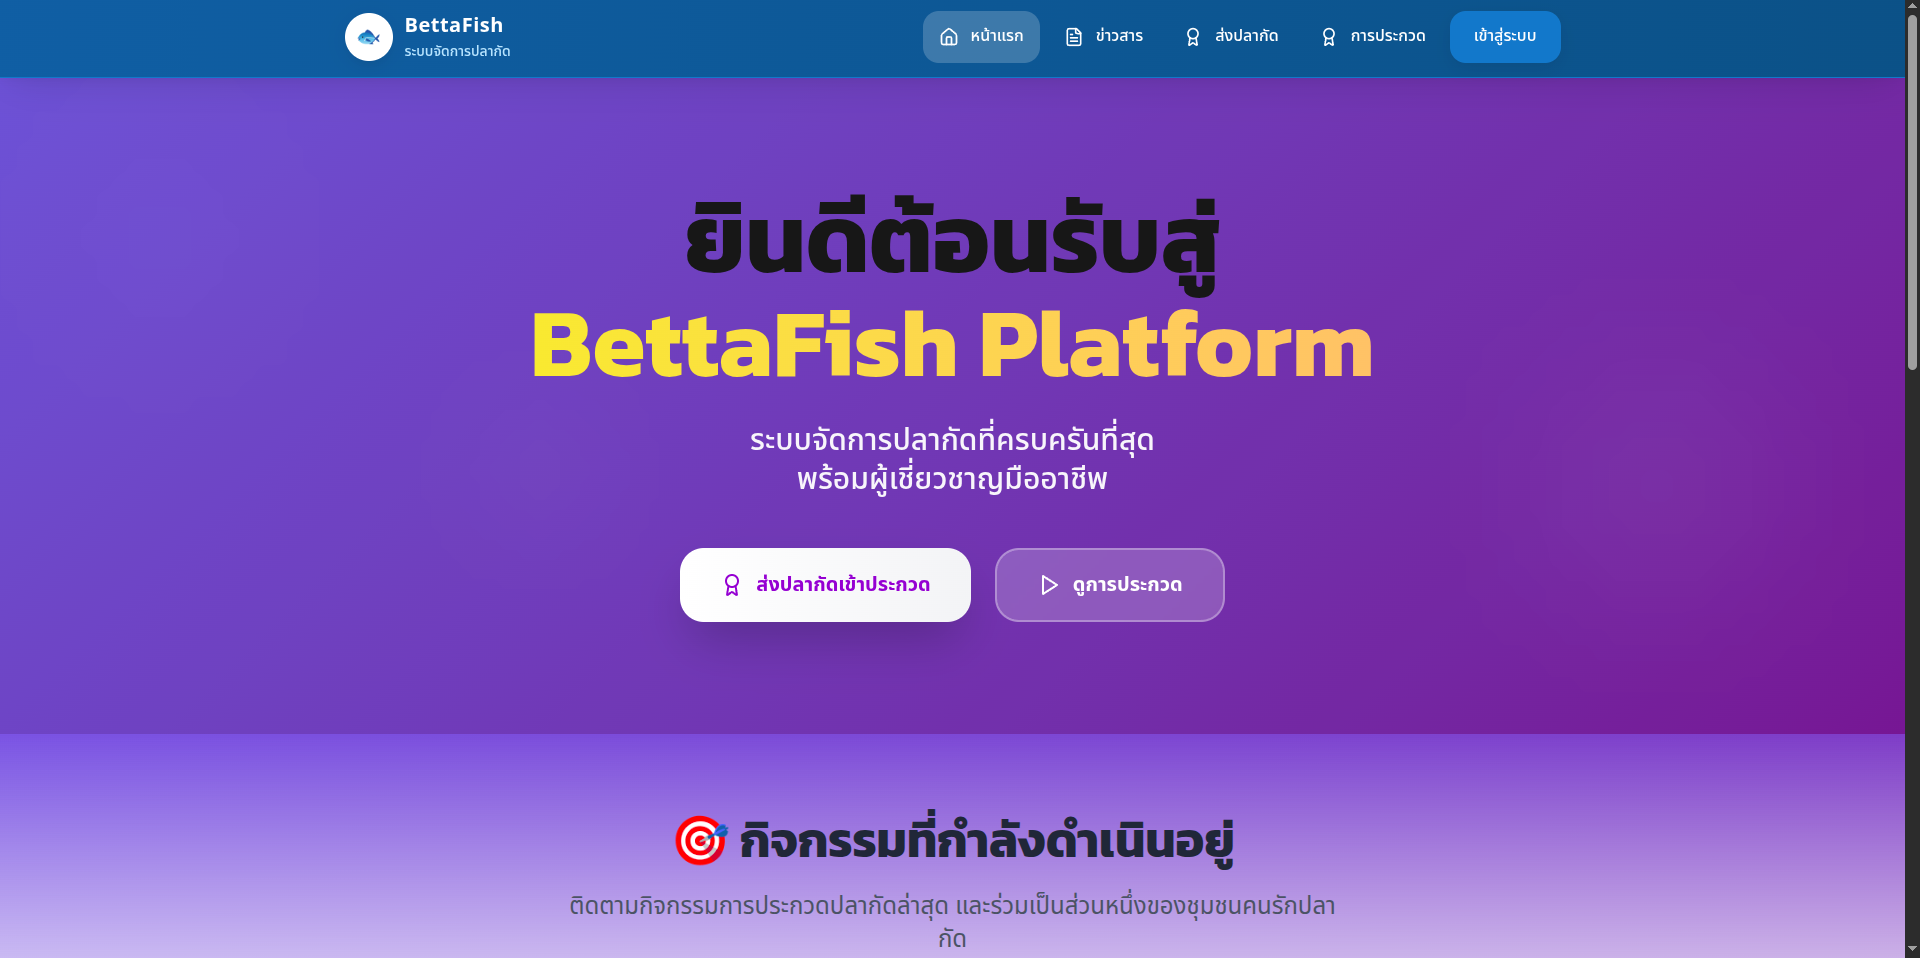
\includegraphics[width=0.8\linewidth]{HP1}
	\caption{หน้าหลักของเว็บไซต์}
\end{figure}

\indent พอเข้ามาที่หน้าแรกผู้ใช้จะเจอเป็นหน้าต้อนรับหลักของเว็บ ตรงส่วนบนสุดจะมีปุ่มให้เลือกใช้งานได้ 3 ปุ่ม
คือ "ส่งปลากัดเข้าประกวด" ถ้ากดปุ่มนี้ก็จะเข้าไปหน้ากรอกข้อมูลเพื่อส่งปลากัดของเราไปให้ผู้เชี่ยวชาญดู หรือส่งเข้าแข่งขันได้เลย กับอีกปุ่มคือ "ดูการประกวด" ที่จะพาไปดูว่าตอนนี้มีประกวดอะไรเปิดรับสมัครอยู่บ้าง จะมีส่วนที่เป็นรูปภาพสไลด์โชว์ (Carousel) โชว์กิจกรรมเด่นๆ ที่กำลังมีอยู่ เราสามารถกดลูกศรซ้าย-ขวาเพื่อเลื่อนดูโปสเตอร์กิจกรรมอื่นๆ ได้ หรือถ้าสนใจกิจกรรมไหนเป็นพิเศษ ก็คลิกที่รูปโปสเตอร์นั้นเพื่อเข้าไปอ่านรายละเอียดของการประกวดได้เลย ในส่วนล่างของหน้า ก็จะมีส่วนของ "ข่าวสารแนะนำ" ครับ จะเป็นการ์ดข่าวต่างๆ เราสามารถคลิกเข้าไปอ่านเนื้อหาข่าวเต็มๆ ของเรื่องที่เราสนใจได้เลย

\newpage

\begin{figure}[h]
	\centering
	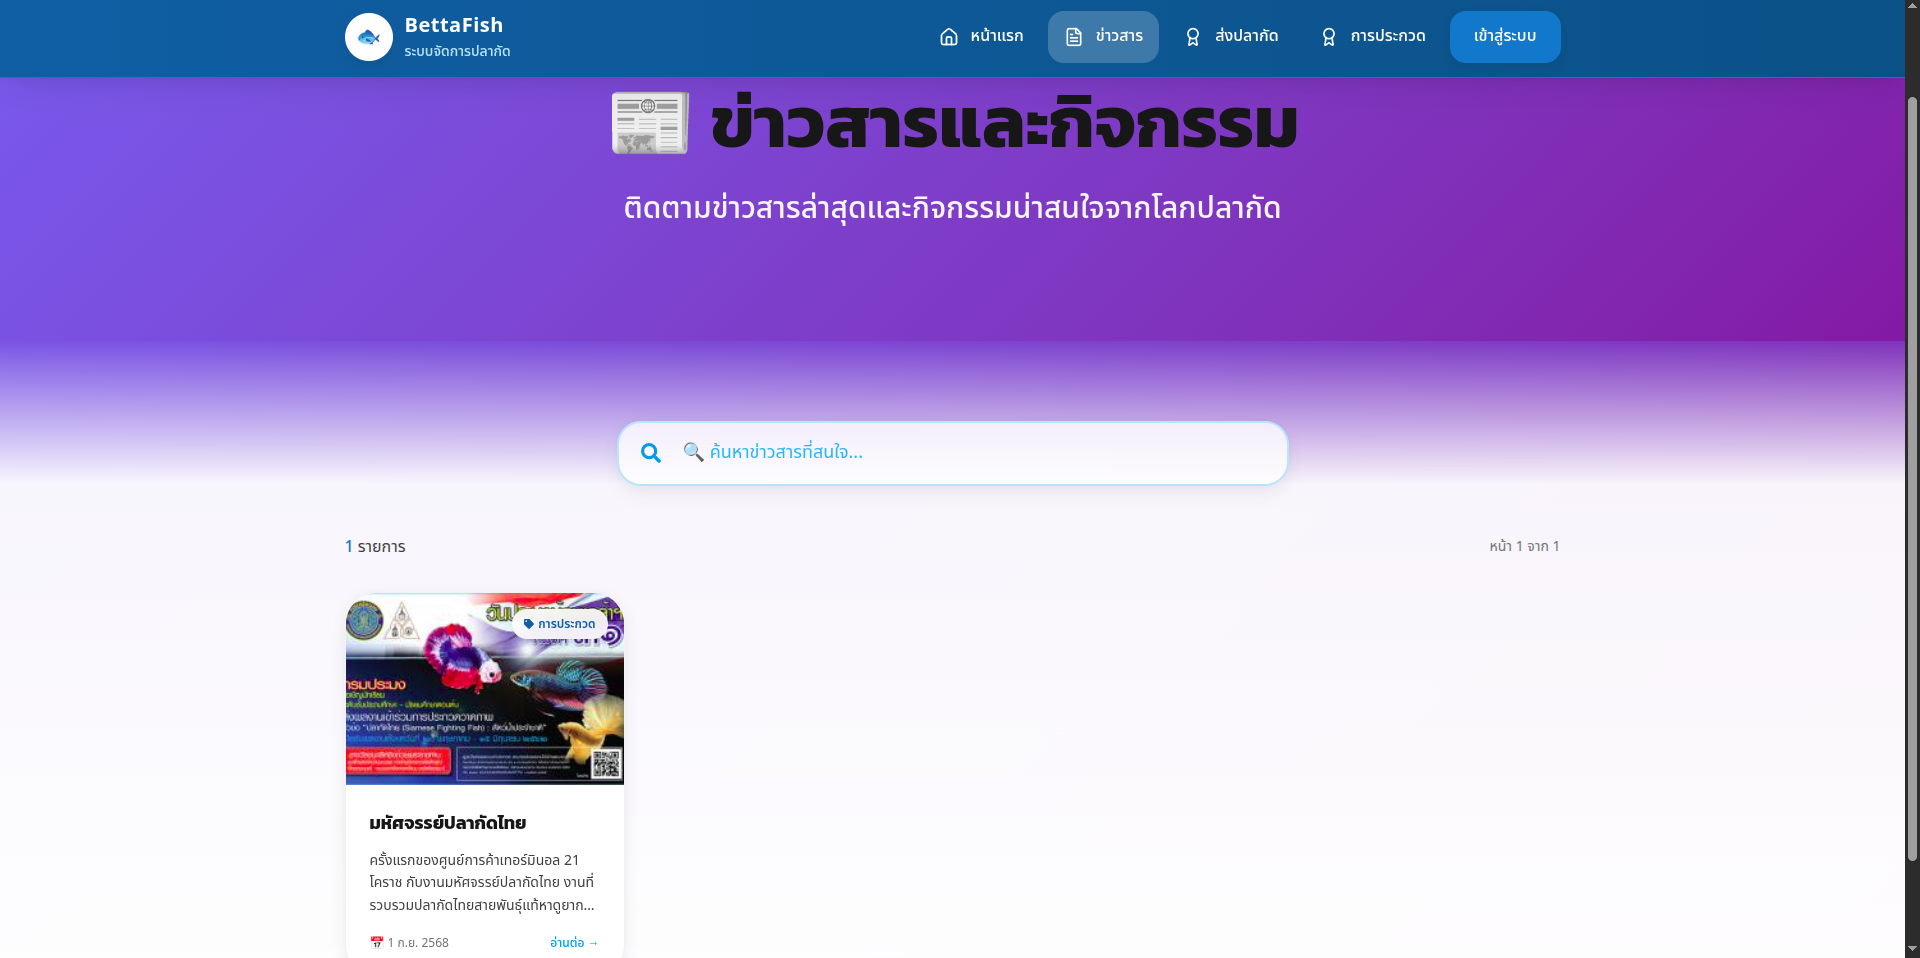
\includegraphics[width=0.8\linewidth]{HP2}
	\caption{หน้าข่าวสารทั้งหมดในระบบ}
\end{figure}

\indent ในหน้านี้ ผู้ใช้จะเจอกับรายการ "ข่าวสารและกิจกรรม" ทั้งหมดที่มีในระบบ โดยหลักๆ แล้ว ผู้ใช้จะสามารถ ค้นหาข่าวที่สนใจ ด้านบนสุดของหน้าจะมีช่องค้นหา ผู้ใช้สามารถพิมพ์คำค้นหาที่ต้องการลงไปได้เลยครับ เช่น ชื่อกิจกรรม หรือคำที่อยู่ในเนื้อหาข่าว ระบบก็จะกรองรายการข่าวที่เกี่ยวข้องมาให้ดูทันที
เลือกอ่านข่าวที่ต้องการ ข่าวแต่ละเรื่องจะแสดงเป็นการ์ดสวยงาม ผู้ใช้สามารถคลิกที่การ์ดข่าวเรื่องไหนก็ได้ที่สนใจ เพื่อเข้าไปอ่านรายละเอียดเนื้อหาทั้งหมดของข่าวนั้นๆ ในหน้าถัดไป
เลื่อนดูหน้าต่างๆ ถ้ามีข่าวเยอะมากๆ จนแสดงไม่หมดในหน้าเดียว ด้านล่างสุดจะมีปุ่มตัวเลขและปุ่ม "ก่อนหน้า" กับ "ถัดไป" ให้ผู้ใช้สามารถกดเพื่อเลื่อนไปดูข่าวในหน้าอื่นๆ ได้ครับ

\vspace{\baselineskip}

\begin{figure}[h]
	\centering
	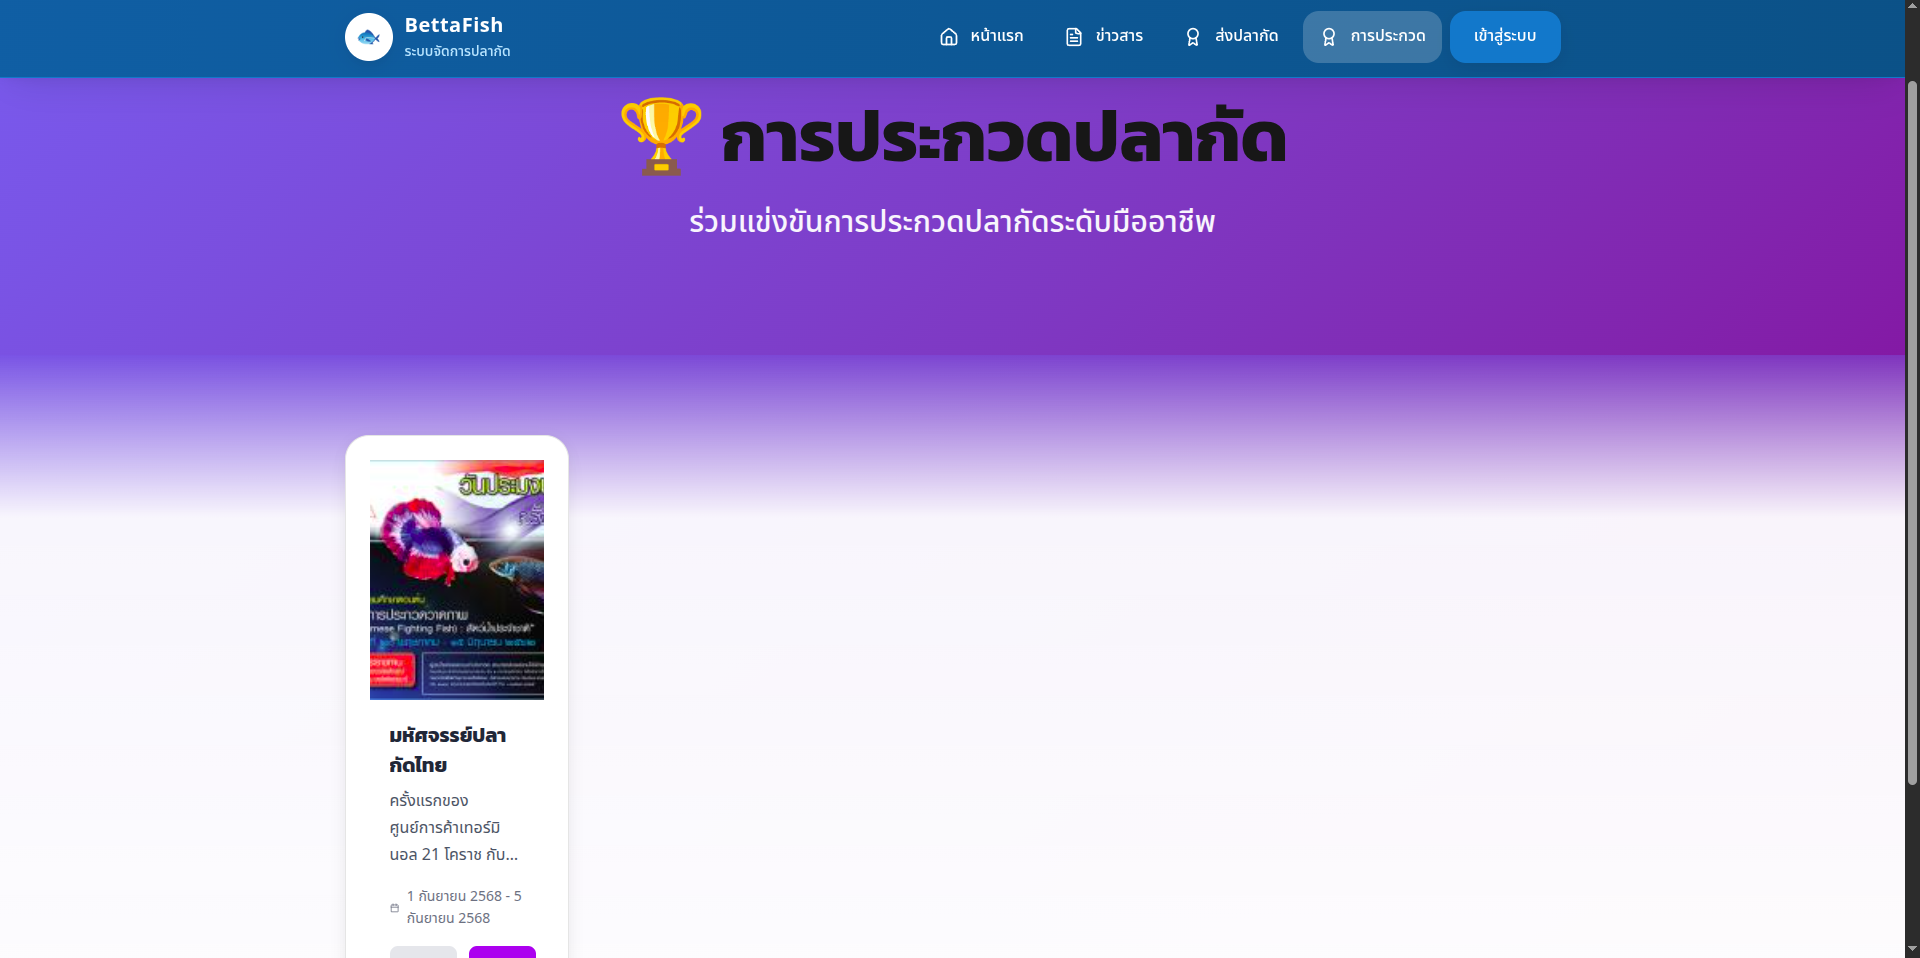
\includegraphics[width=0.8\linewidth]{HP3}
	\caption{หน้ารายการประกวด}
\end{figure}

\indent ในหน้าการประกวด จะแบ่งการใช้งานตามสถานะการล็อกอินของผู้ใช้ \textbf{ถ้ายังไม่ได้ล็อกอิน (ผู้ใช้ทั่วไป)} ดูได้ทุกอย่าง สามารถเข้ามาดูรายการประกวดทั้งหมดที่กำลังเปิดรับสมัครได้ เห็นโปสเตอร์กิจกรรม ชื่อกิจกรรม และรายละเอียดเบื้องต้นได้เหมือนกับคนที่ล็อกอินแล้วทุกอย่างเลย อ่านรายละเอียดได้ แต่จะยังเข้าร่วมไม่ได้ \textbf{ถ้าล็อกอินแล้ว (สมาชิก)} ดูได้ทุกอย่าง และสามารถเข้าร่วมประกวด

\newpage

\begin{figure}[h]
	\centering
	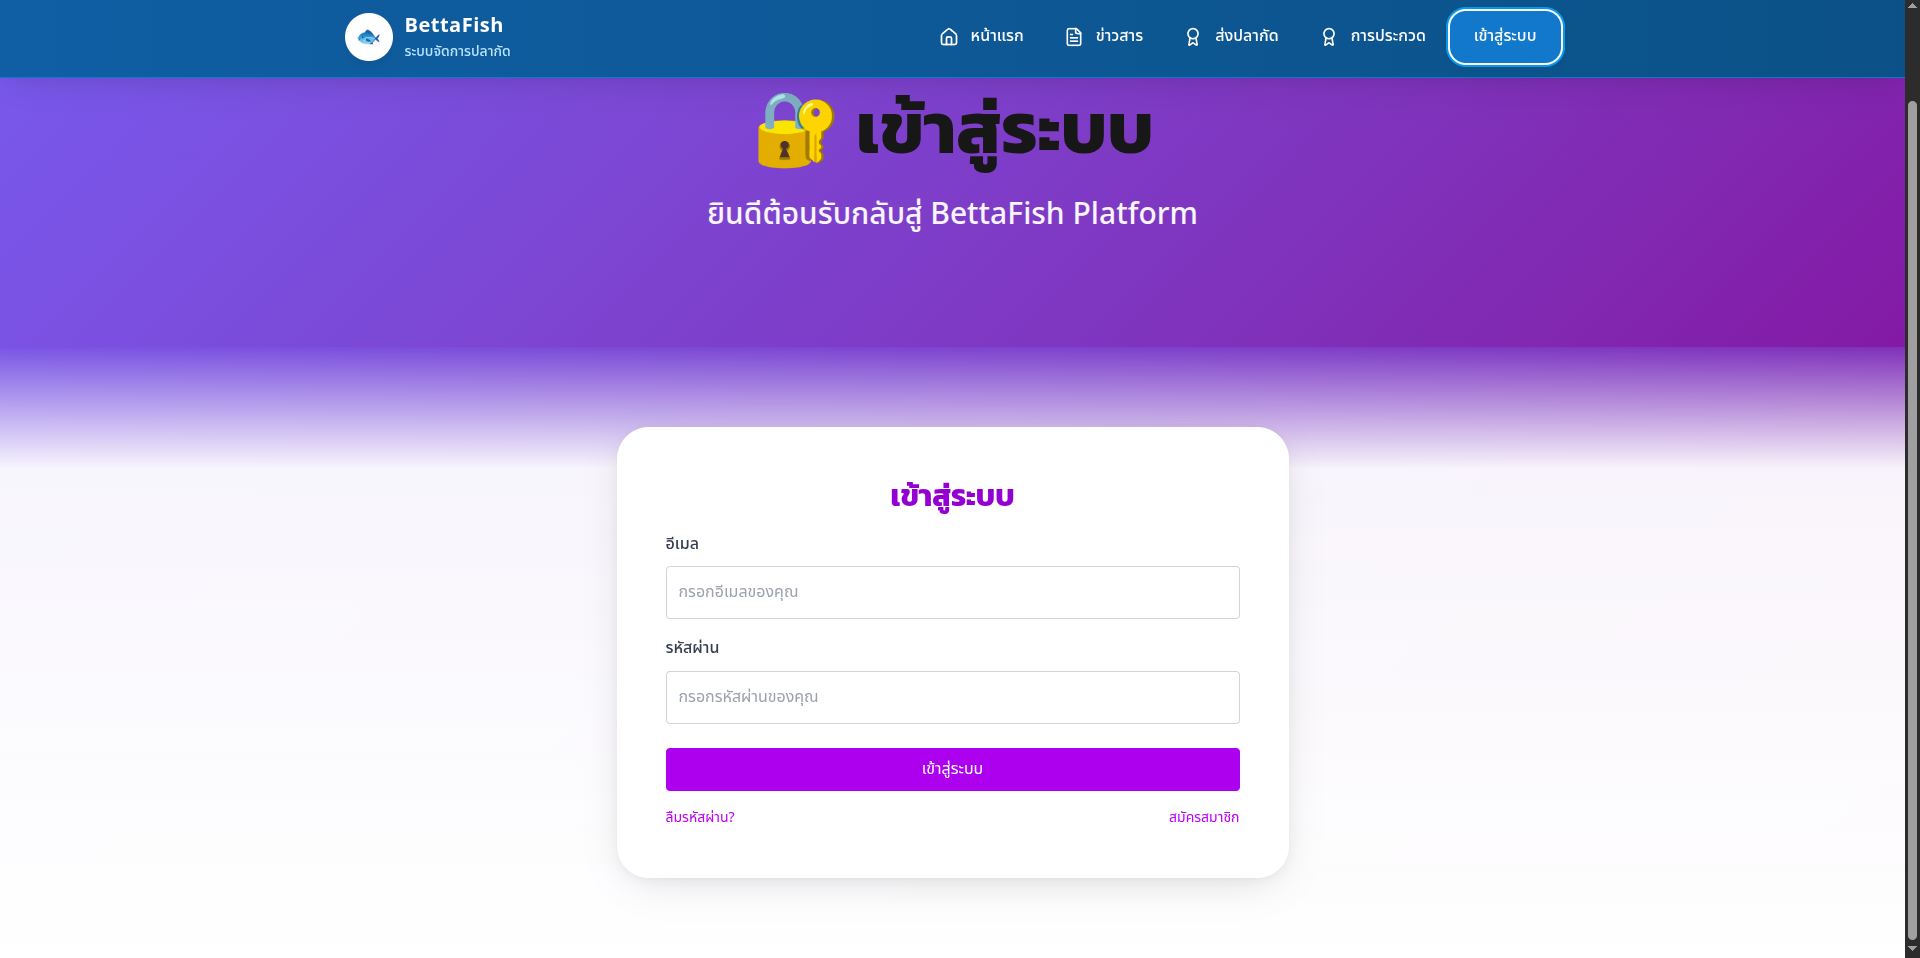
\includegraphics[width=0.8\linewidth]{LG1}
	\caption{หน้าเข้าสู่ระบบ}
\end{figure}

\indent ในหน้านี้ผู้ใช้สามารถเข้าสู่ระบบได้ และสามารถกดสมัครสมาชิกได้ กรณีไม่มีบัญชีเข้าใช้งาน

\vspace{\baselineskip}

\begin{figure}[h]
	\centering
	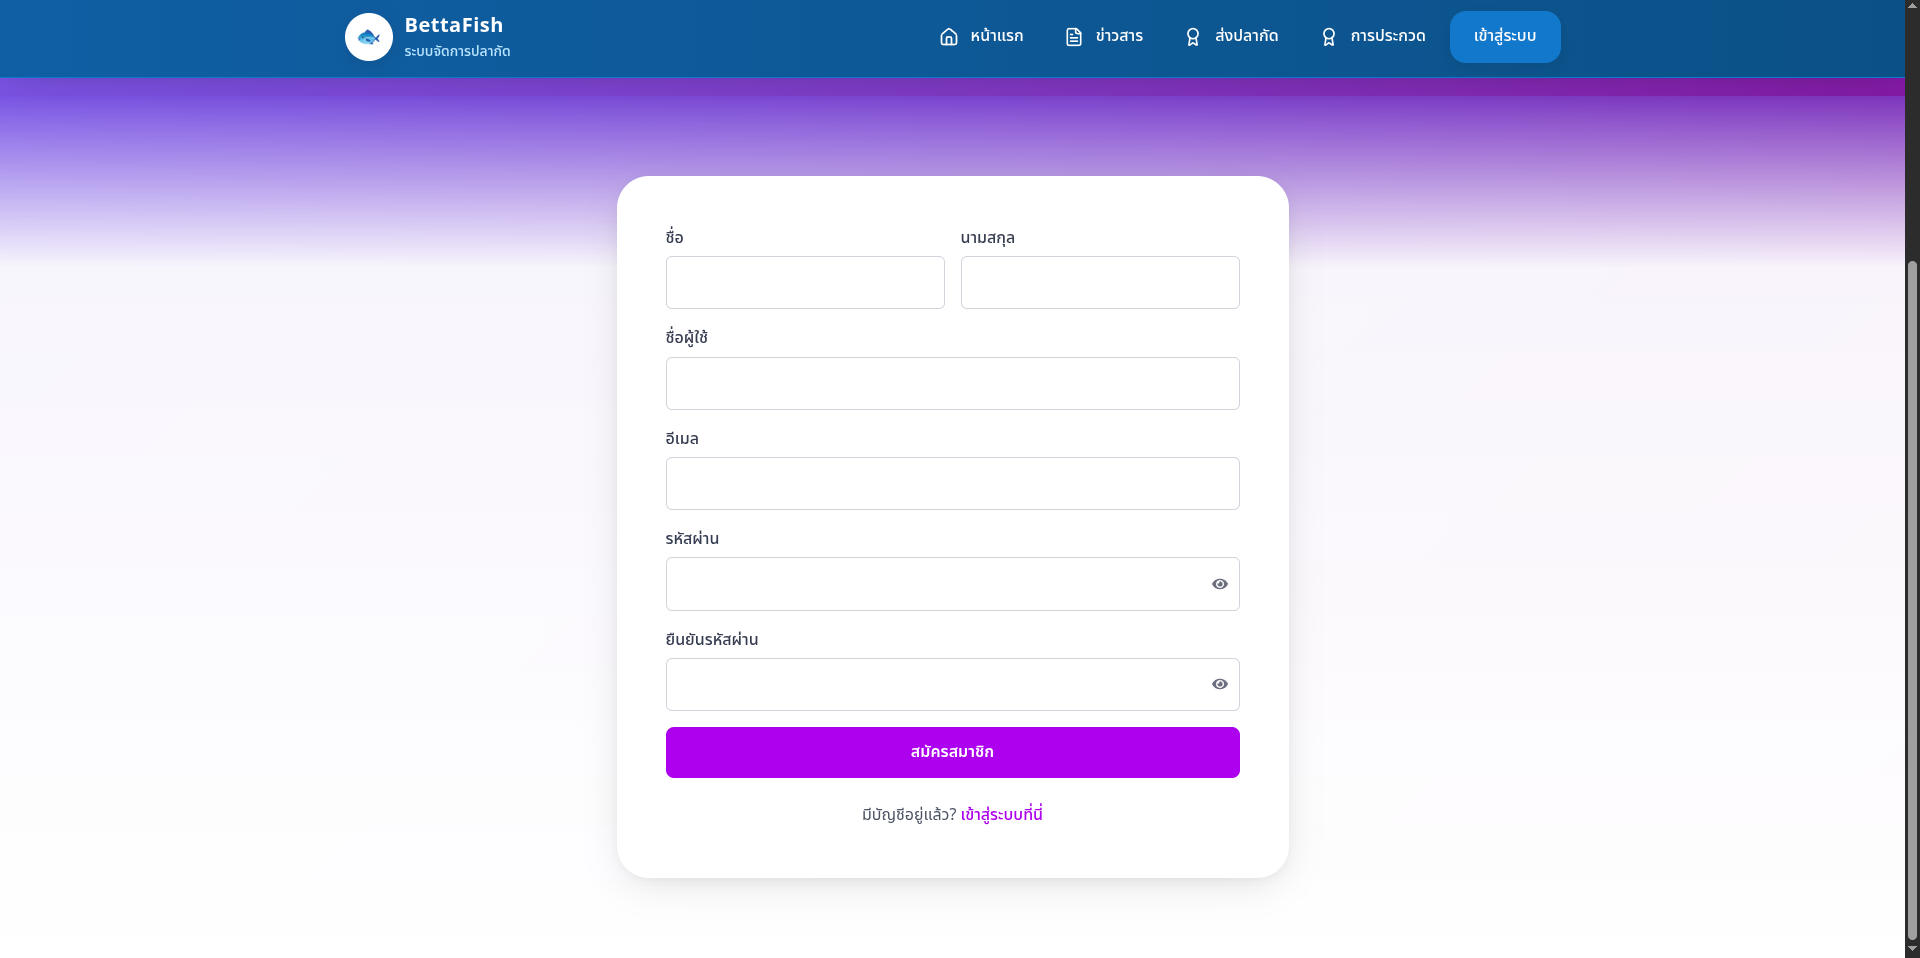
\includegraphics[width=0.8\linewidth]{RG1}
	\caption{หน้าสมัครสมาชิก}
\end{figure}

\indent ในหน้านี้ผู้ใช้สามารถสมัครสมาชิกได้โดยกรอกรายละเอียดตามแบบฟอร์มได้เลย

\newpage

\begin{figure}[h]
	\centering
	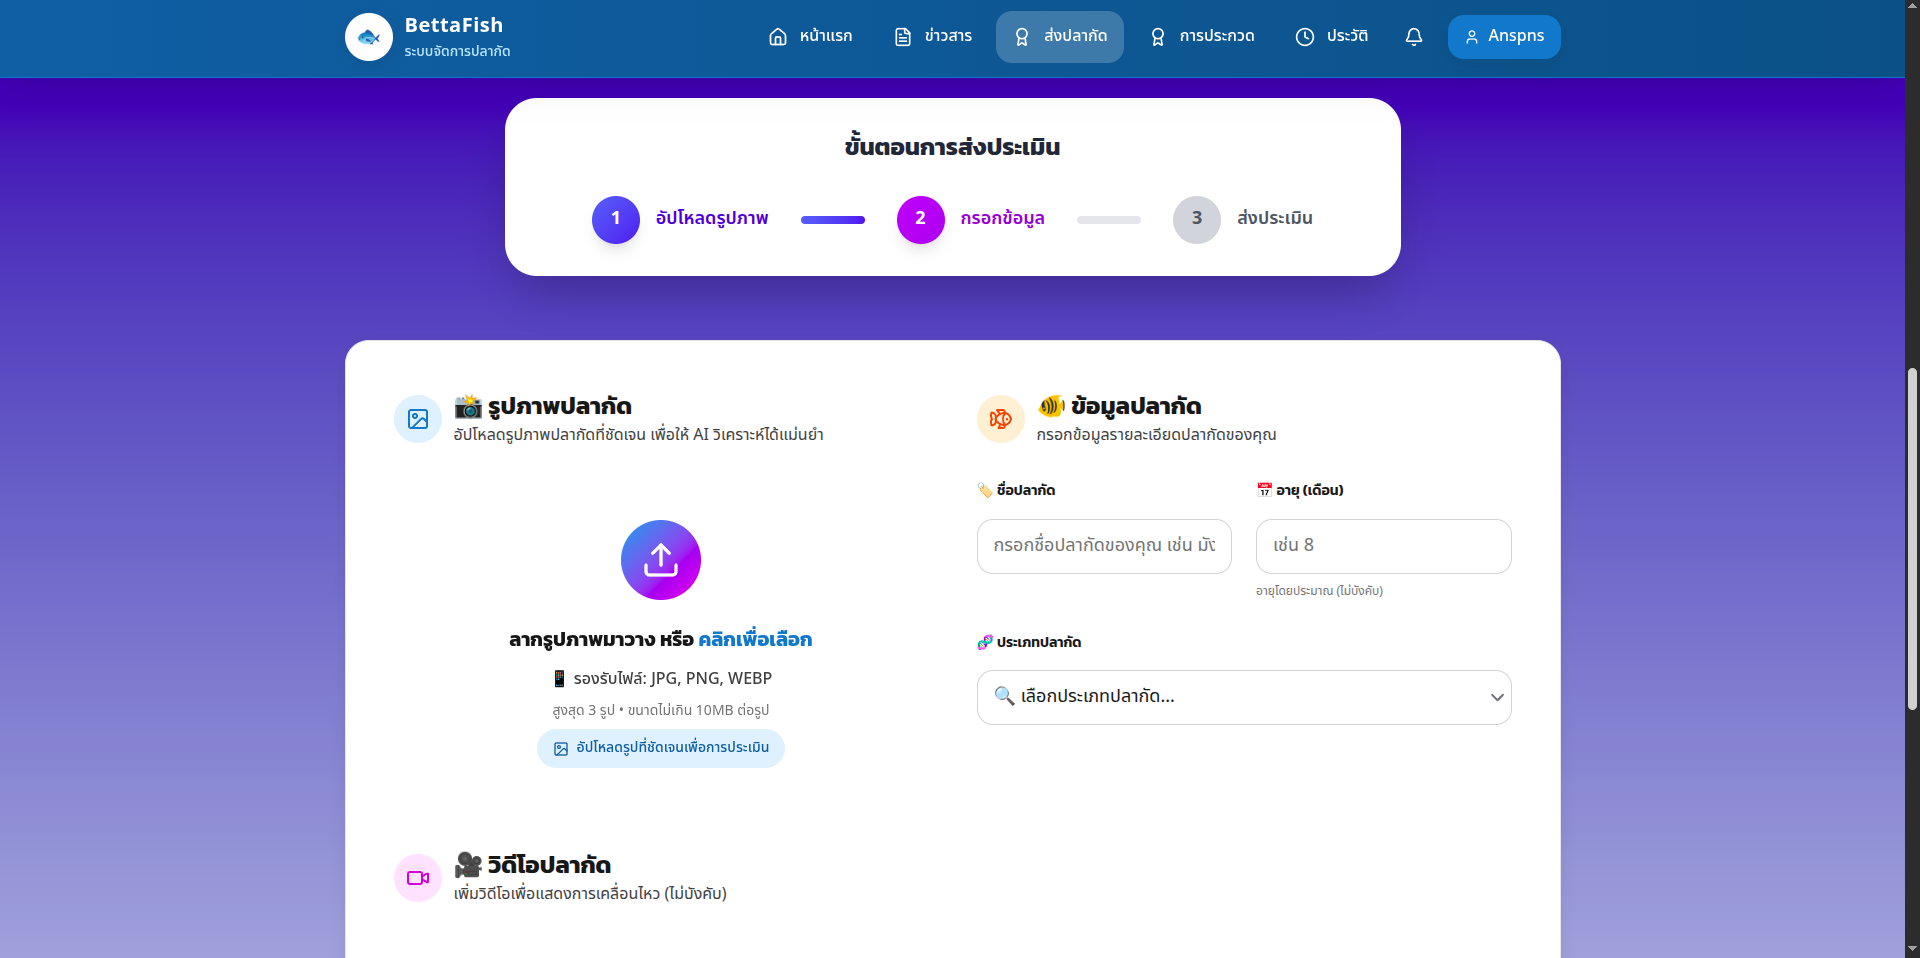
\includegraphics[width=0.8\linewidth]{EV1}
	\caption{หน้าประเมินคุณภาพปลากัด}
\end{figure}

\indent ในหน้านี้ผู้ใช้สามารถใส่ข้อมูลตามแบบฟอร์มได้เลย เช่นใส่รูปภาพ ใส่วิดีโอ ใส่ชื่อปลากัด ใส่ประเภทปลากัด เรามี Ai ช่วยตรวจสอบประเภทปลากัดตอนนี้เราสามารถทำได้ 3 ประเภท ได้แก่ ปลากัดพื้นบ้านมหาชัย ปลากัดพื้นบ้านภาคอีสานหางลาย และปลากัดพื้นบ้านภาคใต้

\vspace{\baselineskip}

\begin{figure}[h]
	\centering
	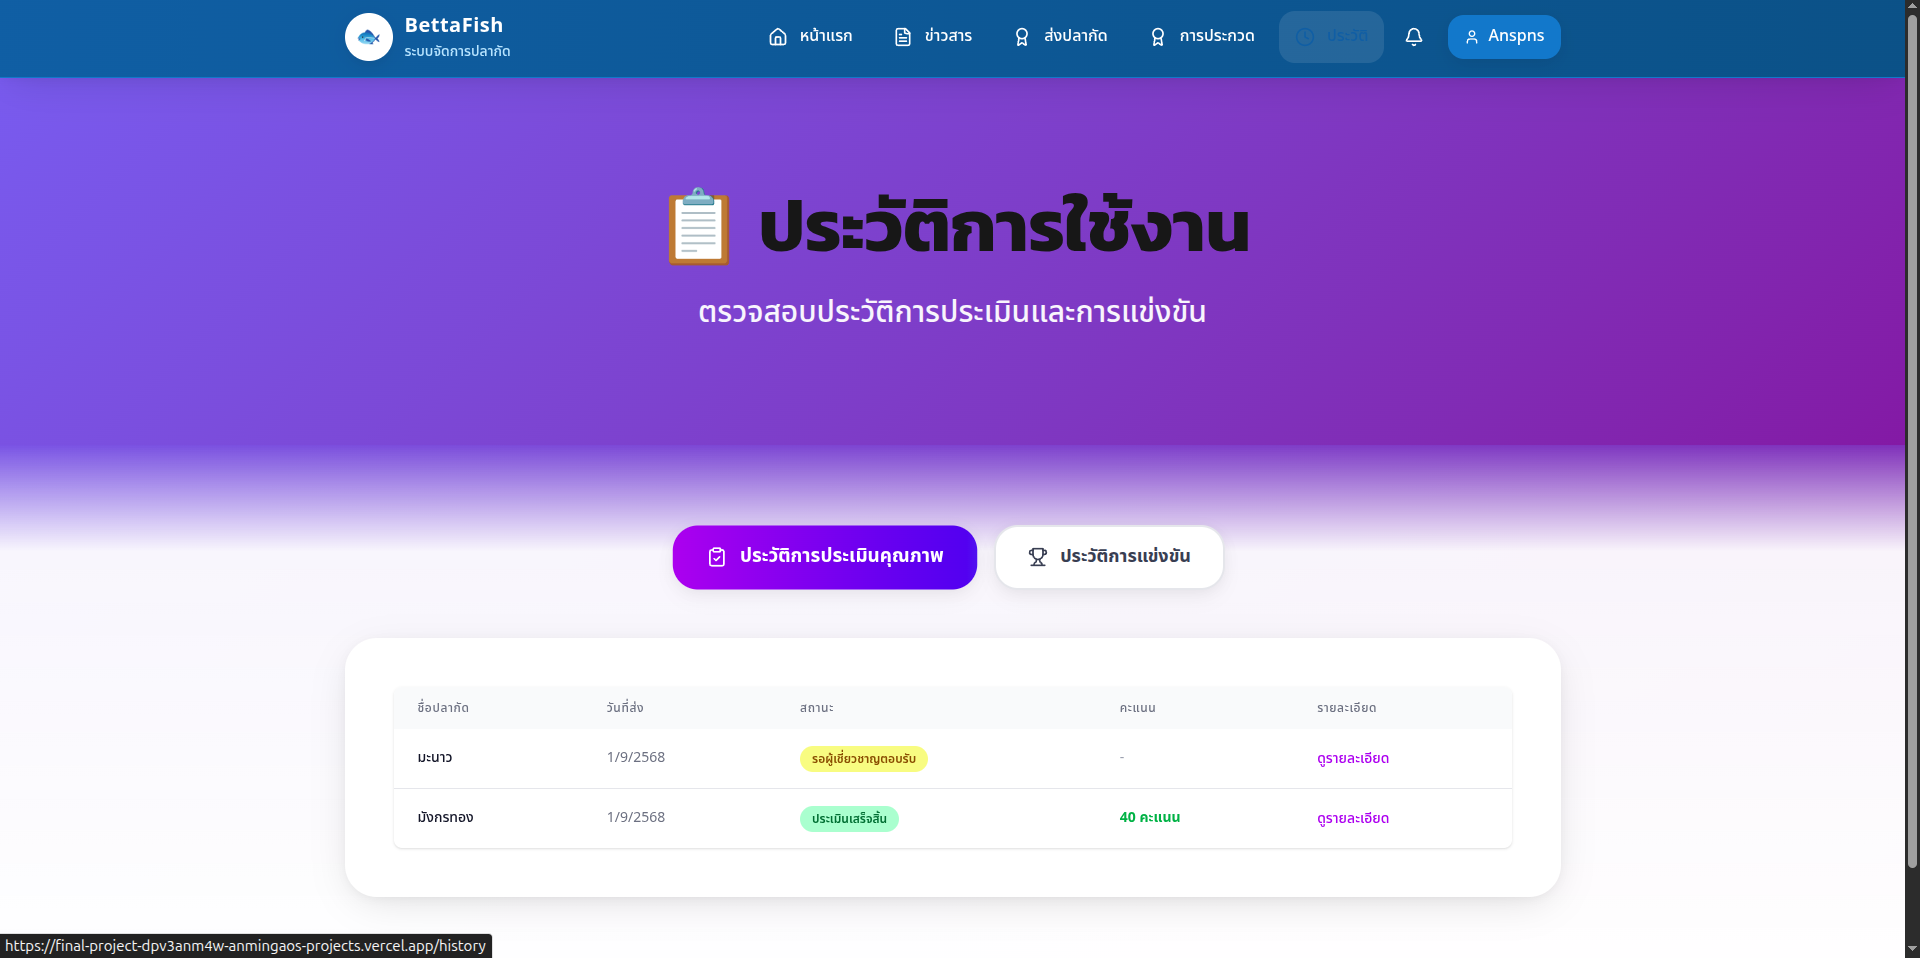
\includegraphics[width=0.8\linewidth]{HT1}
	\caption{หน้าประวัติการส่งประเมินคุณภาพปลากัด}
\end{figure}

\indent ในหน้านี้ผู้ใช้สามารถดูได้ว่าตนเองส่งปลากัดเข้าร่วมการประเมินคุณภาพไปกี่ครั้งแล้ว และสามารถดูคะแนนที่รับได้ 

\newpage

\begin{figure}[h]
	\centering
	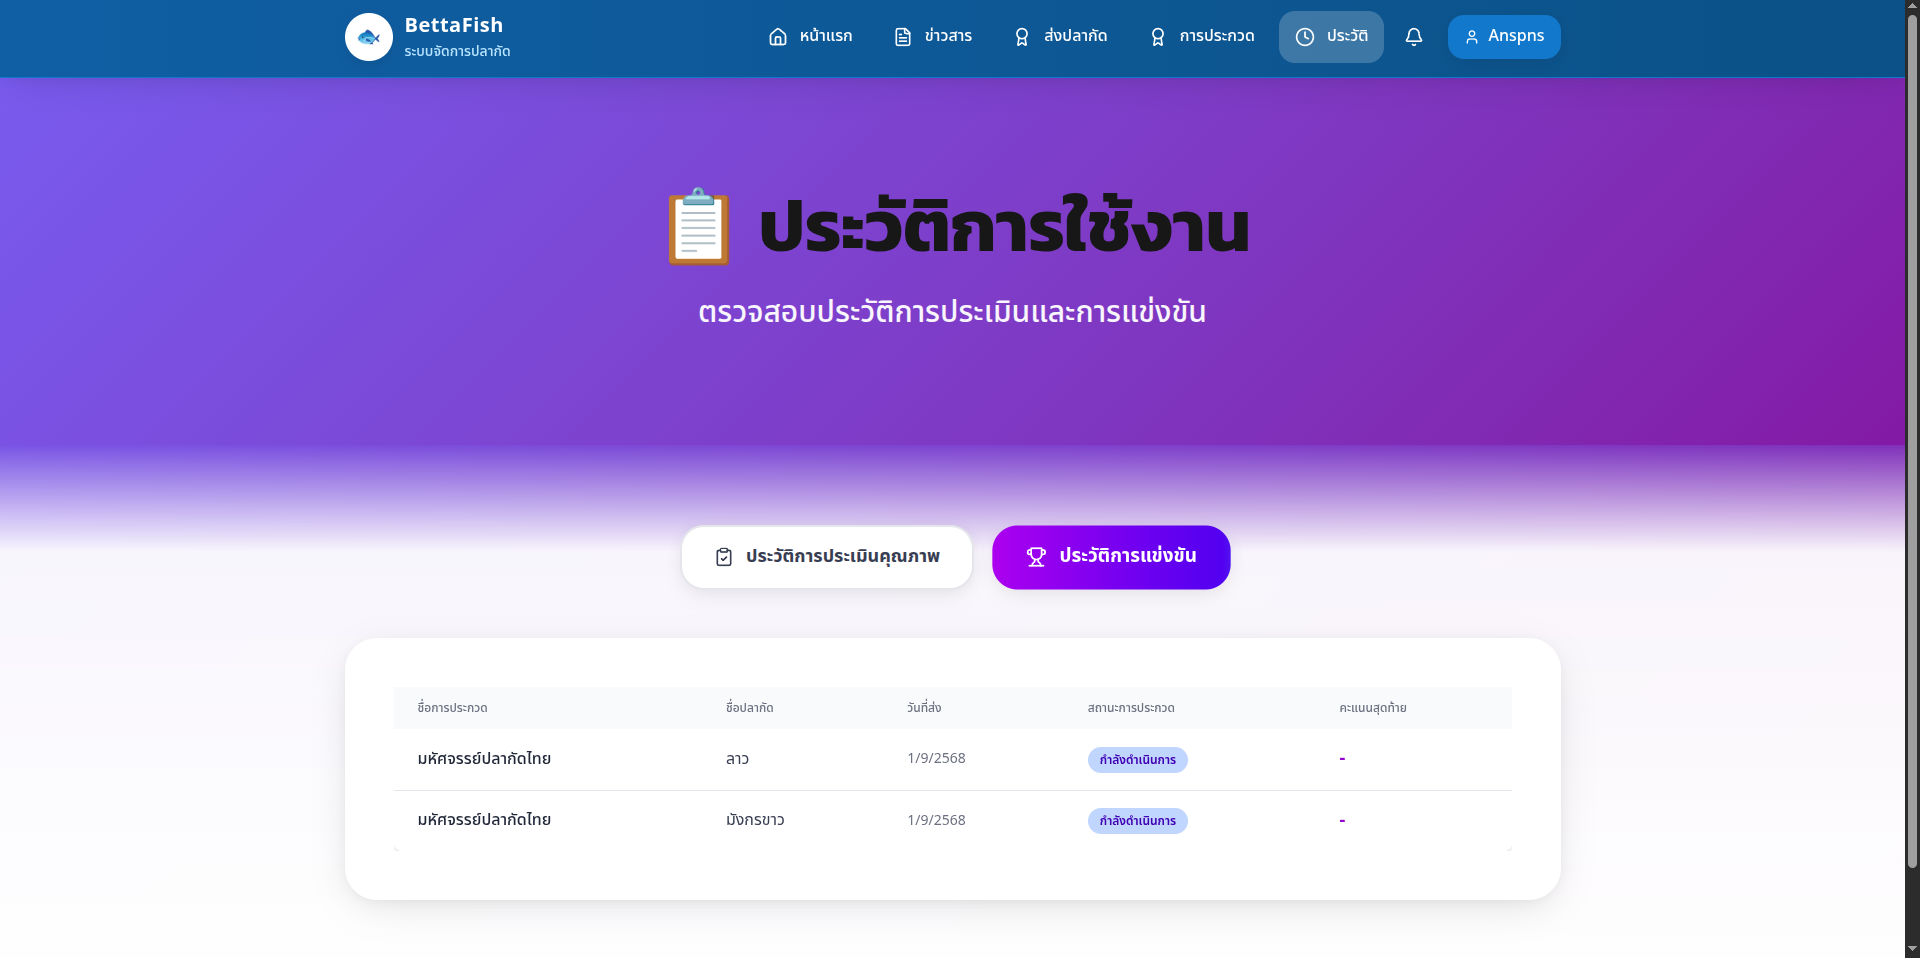
\includegraphics[width=0.8\linewidth]{HT2}
	\caption{หน้าประวัติการส่งประเมินคุณภาพปลากัด}
\end{figure}

\indent ในหน้านี้ผู้ใช้สามารถดูได้ว่าตนเองส่งปลากัดเข้าร่วมการประเกวดไปกี่ครั้งแล้ว และสามารถดูผลได้ว่าได้ลำดับที่เท่าไหร่

\vspace{\baselineskip}

\begin{figure}[h]
	\centering
	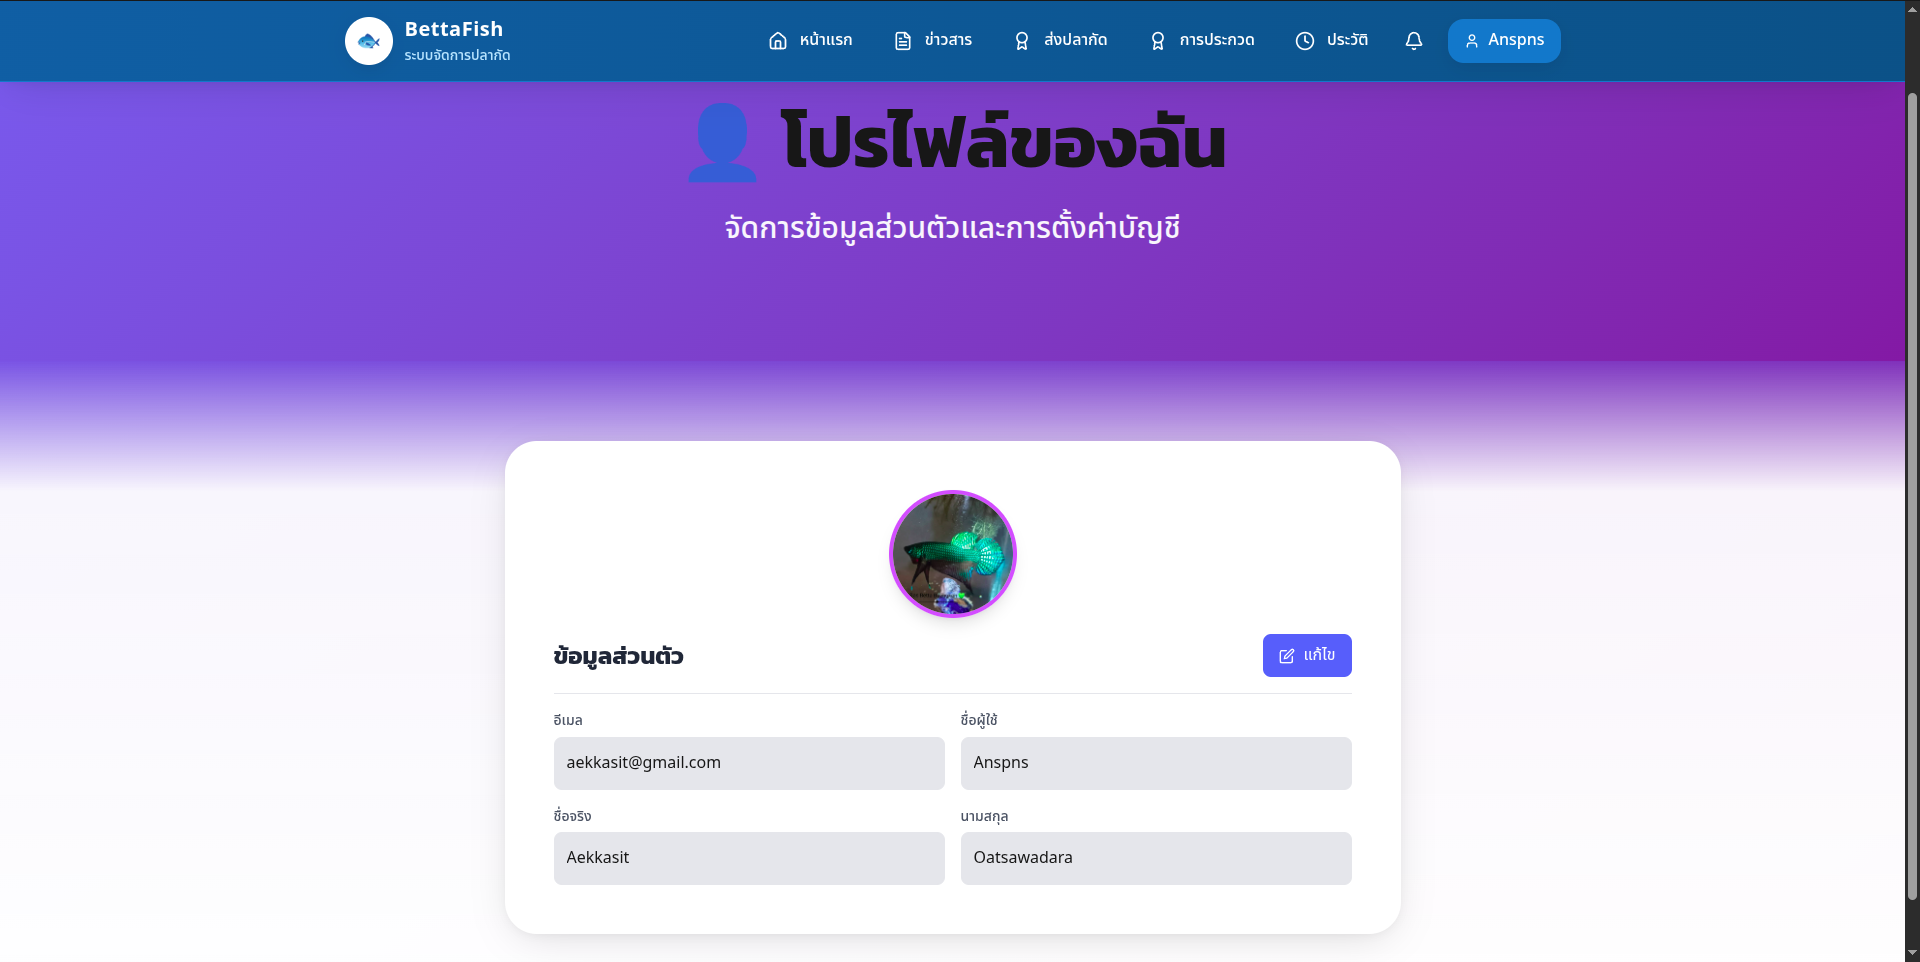
\includegraphics[width=0.8\linewidth]{PF1}
	\caption{หน้าโปรไฟล์ผู้ใช้}
\end{figure}

\indent ในหน้านี้ผู้ใช้สามารถแก้ไขข้อมูลส่วนตัวของตนเองได้และสามารถเปลี่ยบยนรูปภาพโปรไฟล์ได้

\newpage
	
	
\begin{sloppypar}
	\begin{enumerate}[start=2]  % เริ่มที่ 2 (ต่อจาก 1)
		\item \textbf{Web Application ผู้เชี่ยวชาญ}
	\end{enumerate}
\end{sloppypar}

\begin{figure}[h]
	\centering
	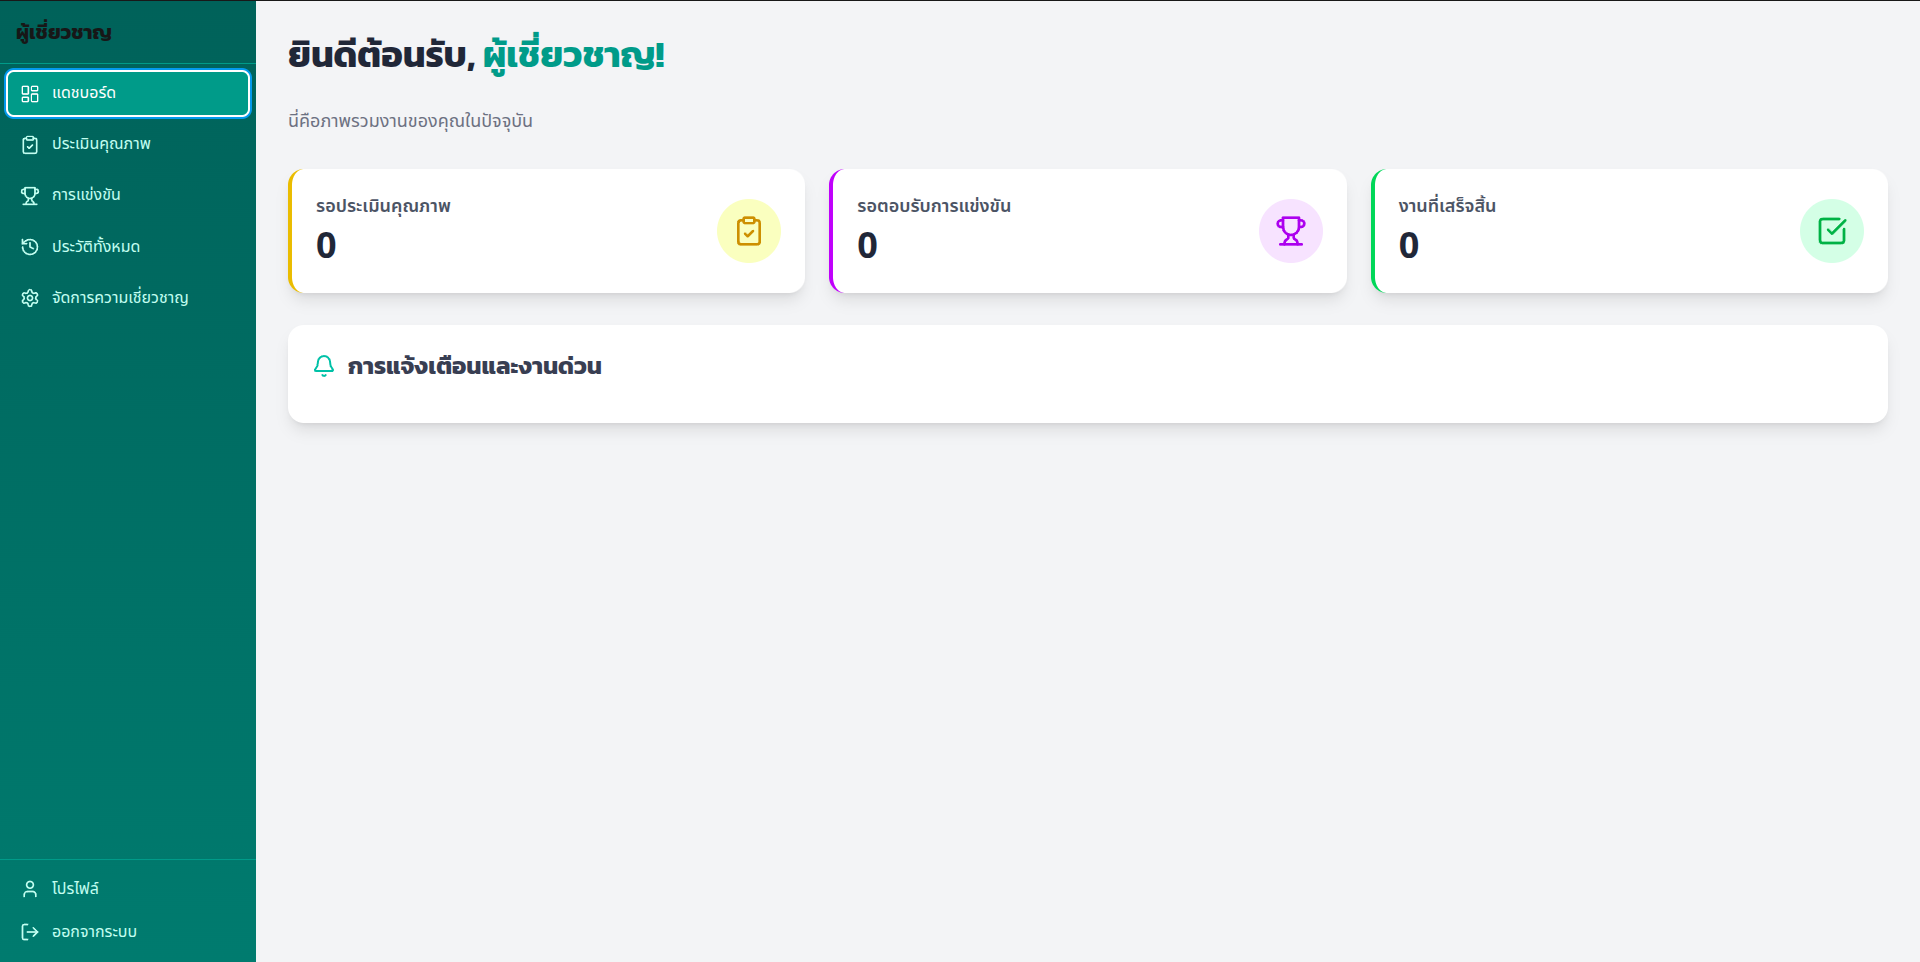
\includegraphics[width=0.8\linewidth]{EP1}
	\caption{หน้าหลักผู้เชี่ยวชาญ}
\end{figure}

\indent ในหน้านี้ ผู้เชี่ยวชาญสามารถ ดูภาพรวมของงานทั้งหมด ได้อย่างรวดเร็วผ่านการ์ดสรุป 3 อันหลักๆ คือ 
"รอประเมินคุณภาพ" บอกจำนวนปลากัดที่ถูกส่งมาให้ประเมินและกำลังรอให้เราจัดการ
"รอตอบรับการแข่งขัน" บอกจำนวนการแข่งขันที่ผู้จัดการ (Manager) ได้ส่งคำเชิญมาให้เราเป็นกรรมการ
"งานที่เสร็จสิ้น" สรุปจำนวนงานทั้งหมดที่เราได้ประเมินหรือตัดสินไปแล้ว 

\vspace{\baselineskip}

\begin{figure}[h]
	\centering
	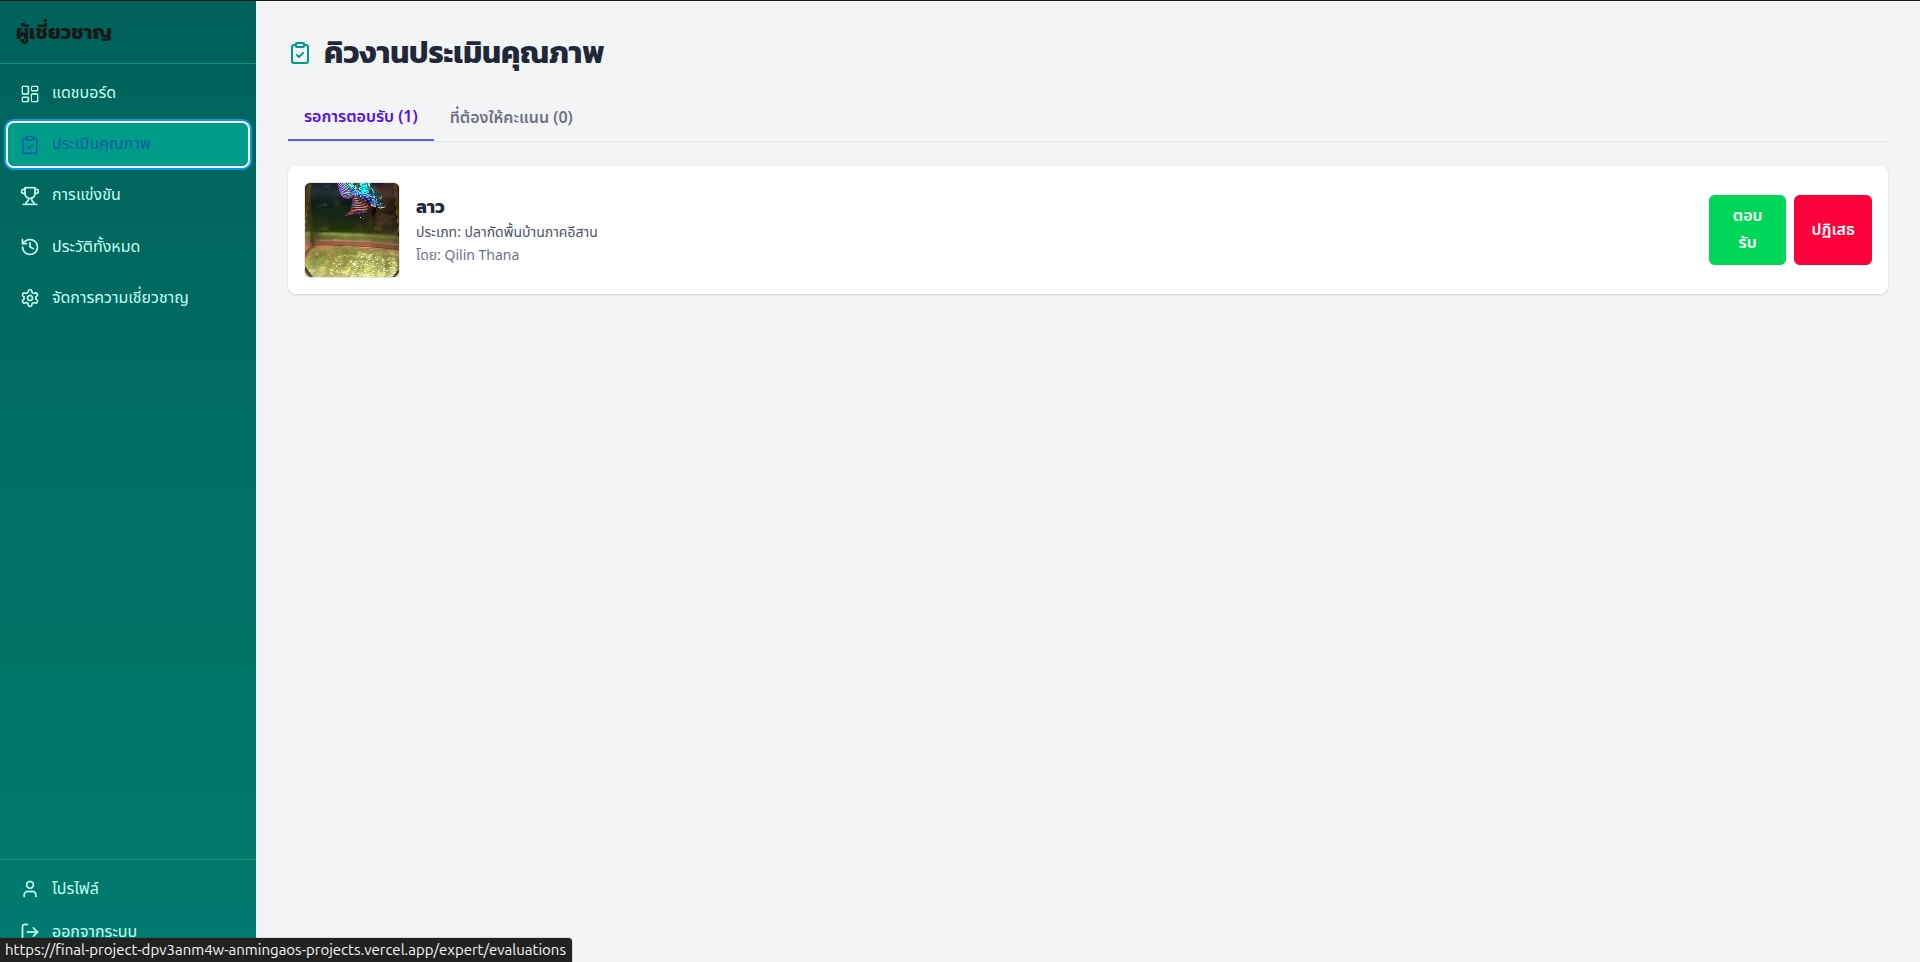
\includegraphics[width=0.8\linewidth]{EP2}
	\caption{หน้าคิวงานผู้เชี่ยวชาญ}
\end{figure}

\indent ในหน้านี้ ผู้เชี่ยวชาญสามารถดูงานที่ได้รับมอบหมาย ผู้เชี่ยวชาญจะเห็นรายการปลากัดที่ระบบมอบหมายมาให้ พร้อมข้อมูลเบื้องต้นอย่างรูปภาพ, ชื่อ, และประเภทของปลา ตัดสินใจรับงาน ผู้เชี่ยวชาญมี 2 ตัวเลือก กดปุ่ม "ตอบรับ" (สีเขียว) เพื่อยืนยันว่าจะทำงานประเมินชิ้นนี้ เมื่องานถูกตอบรับแล้ว ก็จะย้ายไปอยู่ในแท็บ "ที่ต้องให้คะแนน"
กดปุ่ม "ปฏิเสธ" (สีแดง) ในกรณีที่ไม่สะดวกประเมิน หรือเห็นว่าข้อมูลที่ส่งมาไม่เหมาะสม ก็สามารถปฏิเสธงานชิ้นนี้ได้

\endgroup}{}
	\IfFileExists{Chapter3_26.tex}{%==================== chapter3_26.tex ====================

\clearpage
\thispagestyle{plain}

\begingroup
\fontsize{16pt}{19.2pt}\selectfont
\justifying
\XeTeXlinebreakskip=0pt plus 1pt minus 0.5pt
\setlength{\parindent}{1.5cm}
\setlength{\parskip}{0pt}

\begin{figure}[h]
	\centering
	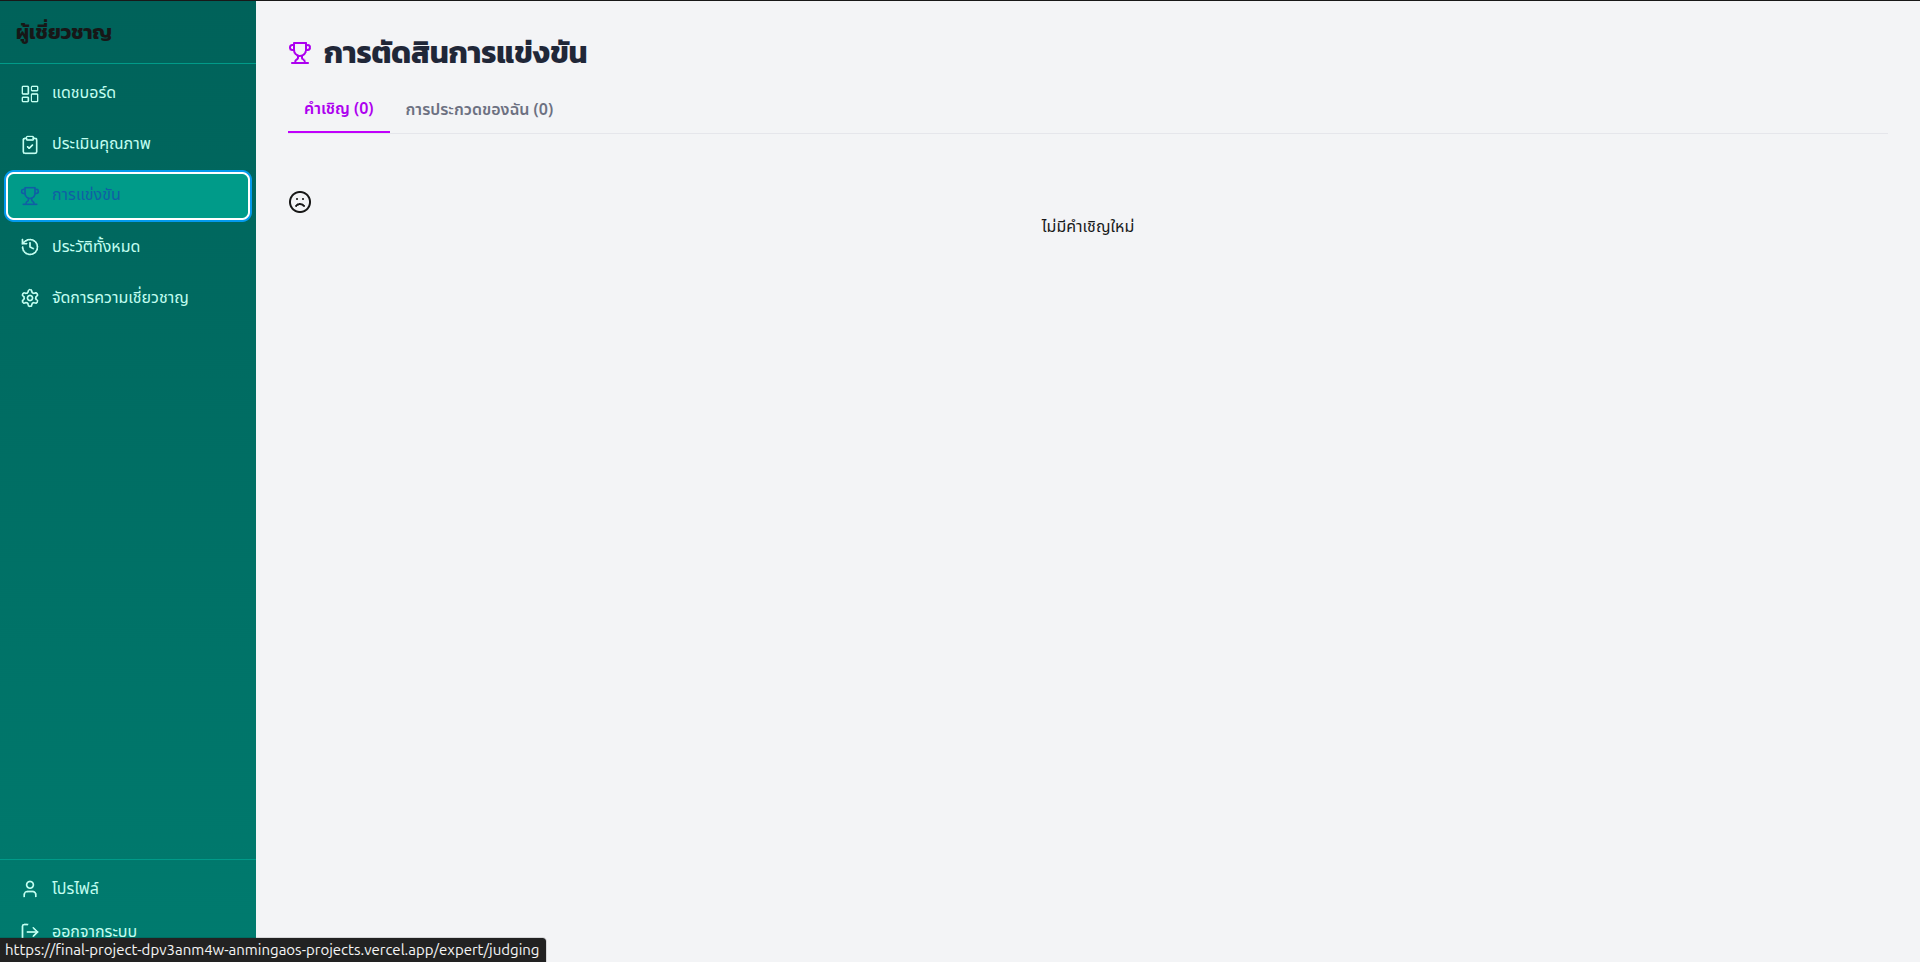
\includegraphics[width=0.8\linewidth]{EP3}
	\caption{หน้ารับงานการเป็นกรรมการ}
\end{figure}

\indent ผู้เชี่ยวชาญจะเห็น รายการคำเชิญใหม่ๆ ที่ผู้จัดการประกวด (Manager) ส่งมาให้เพื่อเป็นกรรมการตัดสิน
ในแต่ละรายการคำเชิญ จะมีปุ่มให้ผู้เชี่ยวชาญตัดสินใจ คือ "ตอบรับ" หรือ "ปฏิเสธ" คำเชิญนั้นๆ 

\vspace{\baselineskip}

\begin{figure}[h]
	\centering
	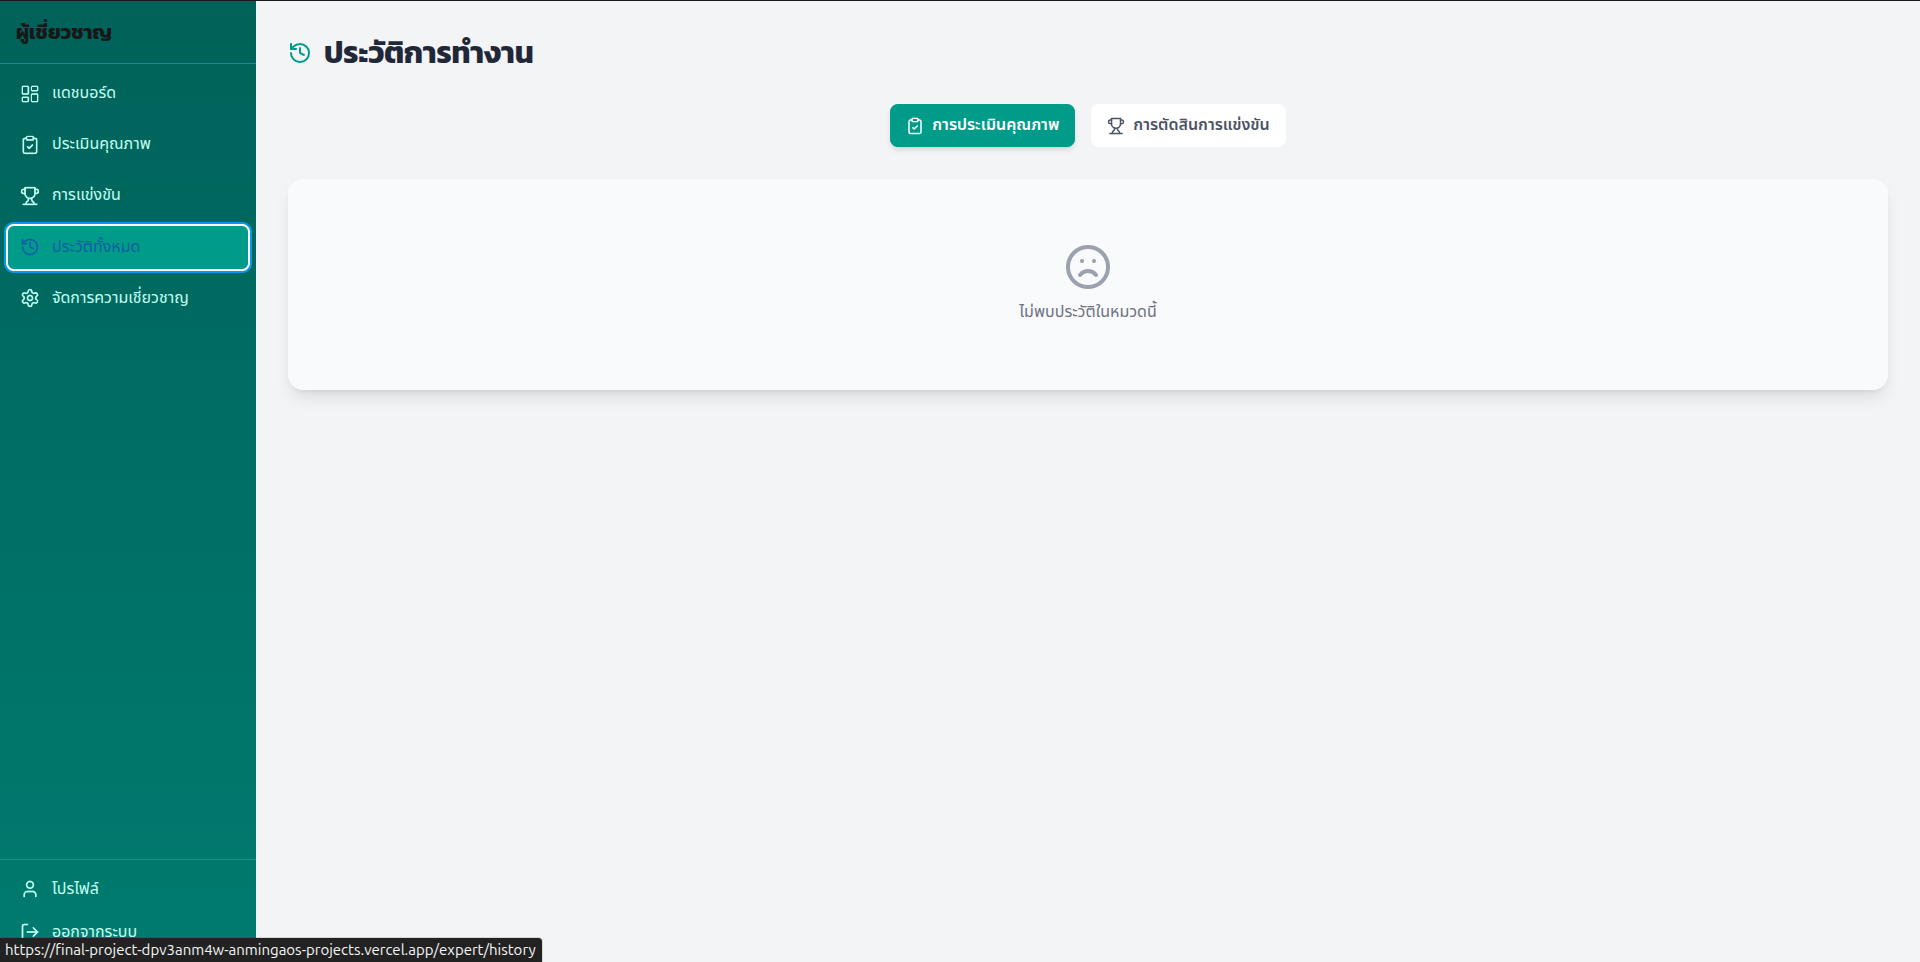
\includegraphics[width=0.8\linewidth]{EP4}
	\caption{หน้าประวัติการทำงาน}
\end{figure}

\indent หน้านี้คือให้ผู้เชี่ยวชาญสามารถ ย้อนกลับมาดูงานทั้งหมดที่เคยทำเสร็จไปแล้วโดยจะมีการแบ่งประวัติออกเป็น 2 ประเภท ซึ่งผู้ใช้สามารถกดเลือกดูได้จากปุ่มด้านบน การประเมินคุณภาพ เมื่อกดปุ่มนี้ (ซึ่งเป็นหน้าที่แสดงในรูป) ผู้เชี่ยวชาญจะเห็น รายการปลากัดที่เคยประเมินคุณภาพไปแล้วทั้งหมด ในรูปแบบตาราง การตัดสินการแข่งขัน 
ถ้ากดปุ่มนี้ ผู้เชี่ยวชาญก็จะเห็น รายชื่อการแข่งขันทั้งหมดที่เคยเข้าไปเป็นกรรมการตัดสิน

\newpage

\begin{figure}[h]
	\centering
	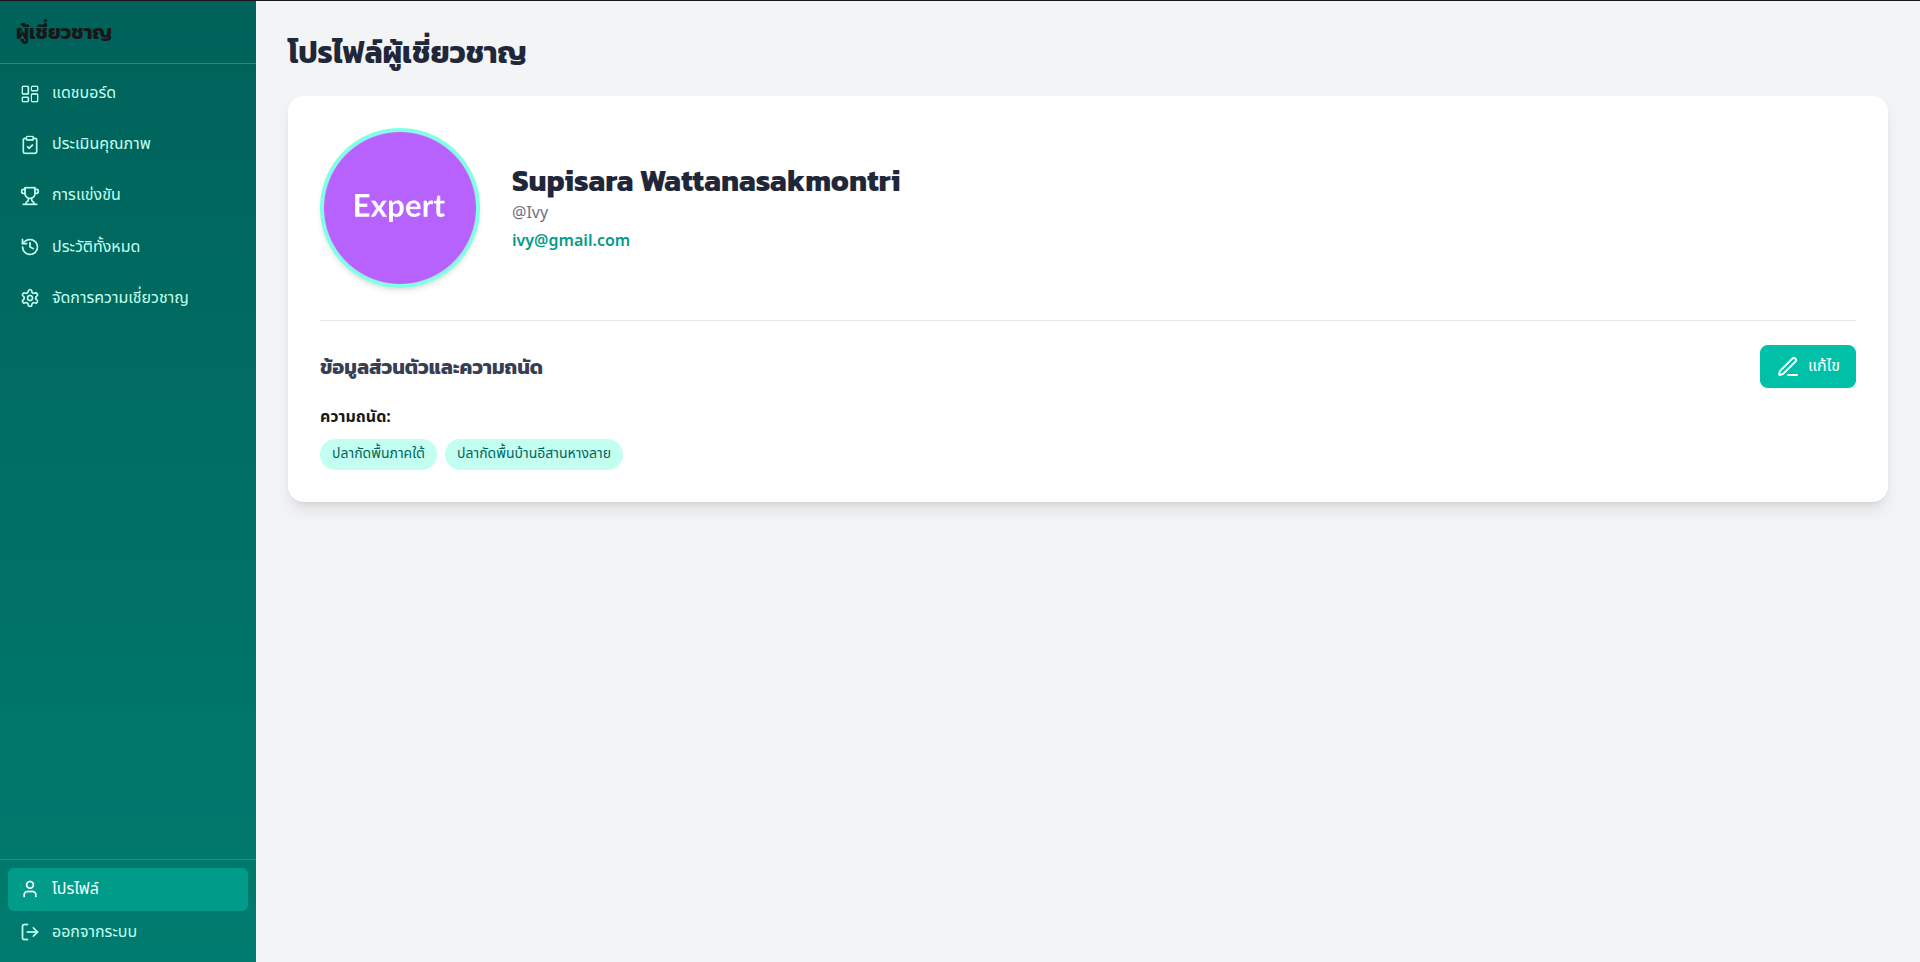
\includegraphics[width=0.8\linewidth]{EP5}
	\caption{หน้าโปรไฟลืผู้เชี่ยวชาญ}
\end{figure}

\indent  เชี่ยวชาญสามารถ ดูและจัดการข้อมูลส่วนตัวของตัวเอง ได้ โดยจะแบ่งการทำงานเป็น 2 ส่วนหลักๆ การดูข้อมูล ในตอนแรกที่เข้ามา ผู้เชี่ยวชาญจะเห็นข้อมูลของตัวเองที่แสดงอยู่ ได้แก่ รูปโปรไฟล์, ชื่อ-นามสกุล, Username และอีเมล ความถนัด (Specialities) จะมีป้าย Tag แสดงประเภทปลากัดที่ตัวเองมีความเชี่ยวชาญเป็นพิเศษ 

\endgroup}{}
	\IfFileExists{Chapter3_27.tex}{%==================== chapter3_27.tex ====================

\clearpage
\thispagestyle{plain}

\begingroup
\fontsize{16pt}{19.2pt}\selectfont
\justifying
\XeTeXlinebreakskip=0pt plus 1pt minus 0.5pt
\setlength{\parindent}{1.5cm}
\setlength{\parskip}{0pt}

\begin{sloppypar}
	\begin{enumerate}[start=4]  % เริ่มที่ 2 (ต่อจาก 1)
		\item \textbf{Web Application ผู้จัดการประกวด}
	\end{enumerate}
\end{sloppypar}

\begin{figure}[h]
	\centering
	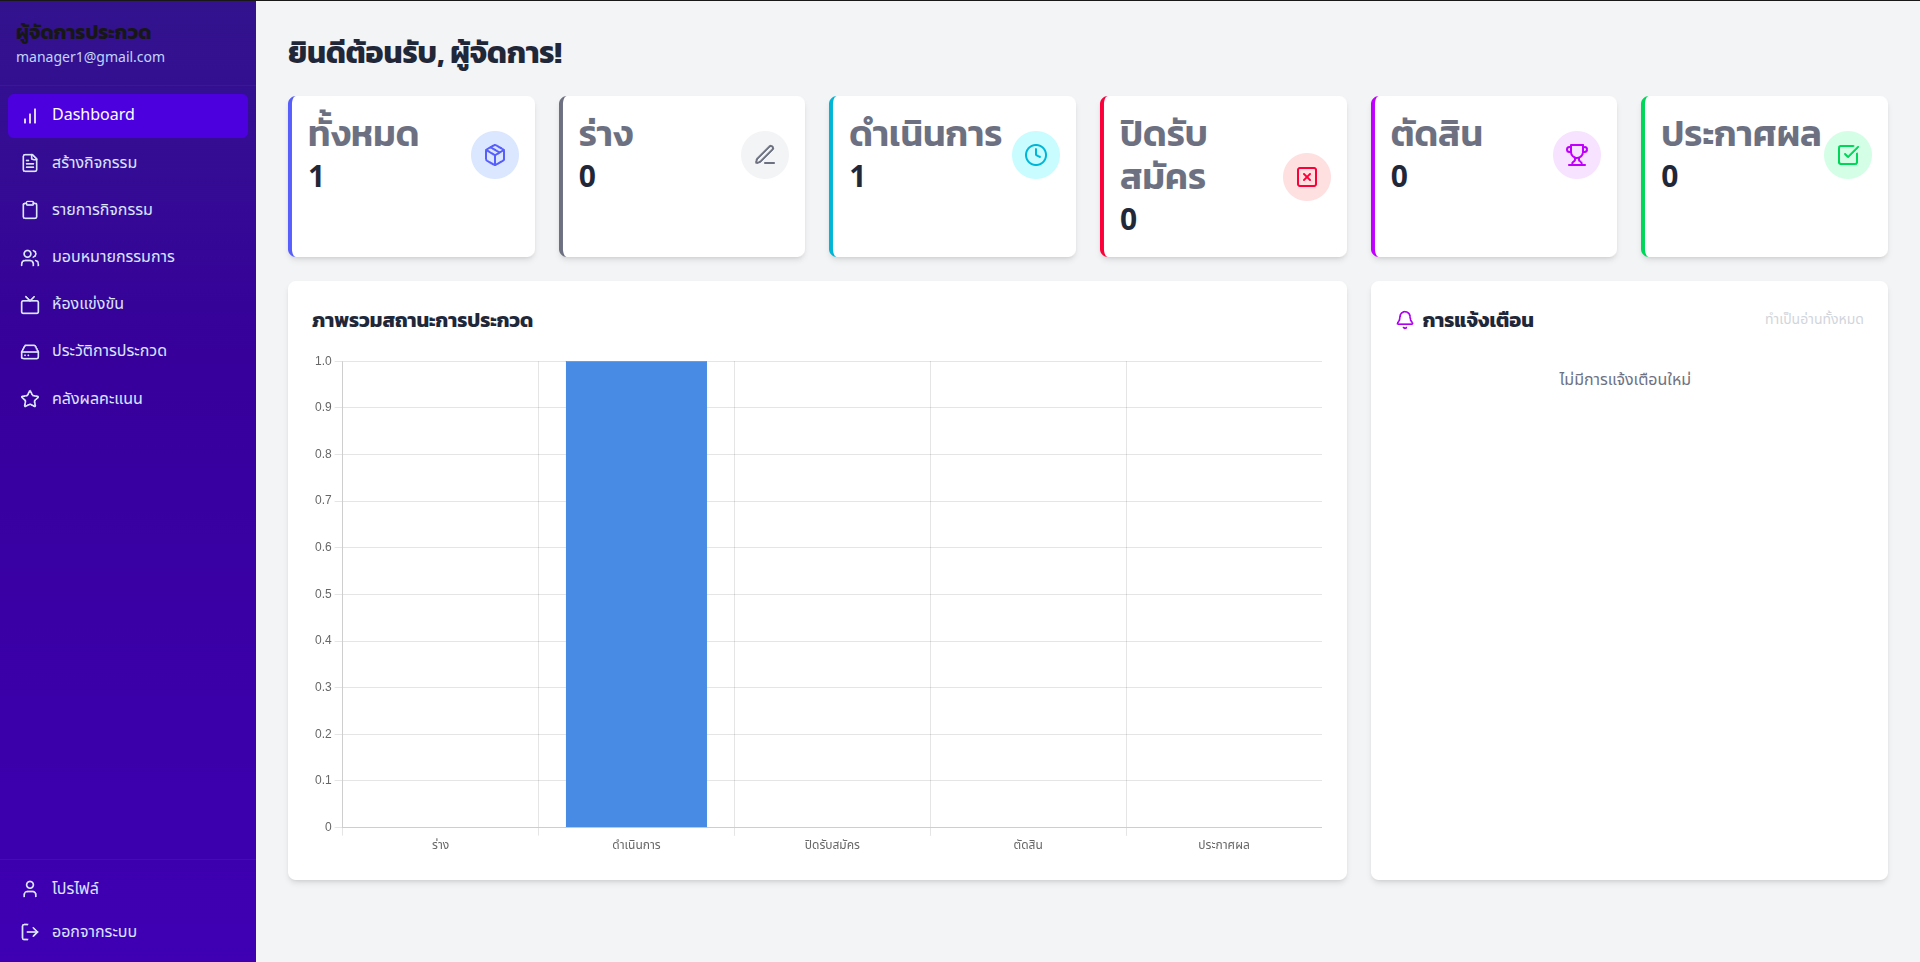
\includegraphics[width=0.8\linewidth]{MG1}
	\caption{หน้าหลักของผู้จัดการประกวด}
\end{figure}

\indent หน้านี้คือหน้า แดชบอร์ด (Dashboard) ผู้จัดการประกวด จัดการสามารถ ดูภาพรวม และ เข้าถึงเครื่องมือจัดการ ทั้งหมดได้ สรุปสถานะการประกวด: ตรงกลางหน้าจะมี การ์ดสรุปตัวเลข บอกชัดเจนว่าตอนนี้มีกิจกรรมทั้งหมดกี่รายการ, อยู่ในสถานะ "ร่าง", "กำลังดำเนินการ", หรือ "ประกาศผล" ไปแล้วกี่รายการ ซึ่งข้อมูลนี้จะถูกสรุปเป็น กราฟแท่ง ด้านล่างเพื่อให้เห็นภาพรวมได้ง่ายขึ้น ดูการแจ้งเตือน: ทางด้านขวาจะมีกล่อง "การแจ้งเตือน" คอยบอกข่าวสารสำคัญๆ เช่น มีผู้เชี่ยวชาญตอบรับคำเชิญ หรือมีกิจกรรมที่ใกล้จะเริ่มแล้ว

\vspace{\baselineskip}

\begin{figure}[h]
	\centering
	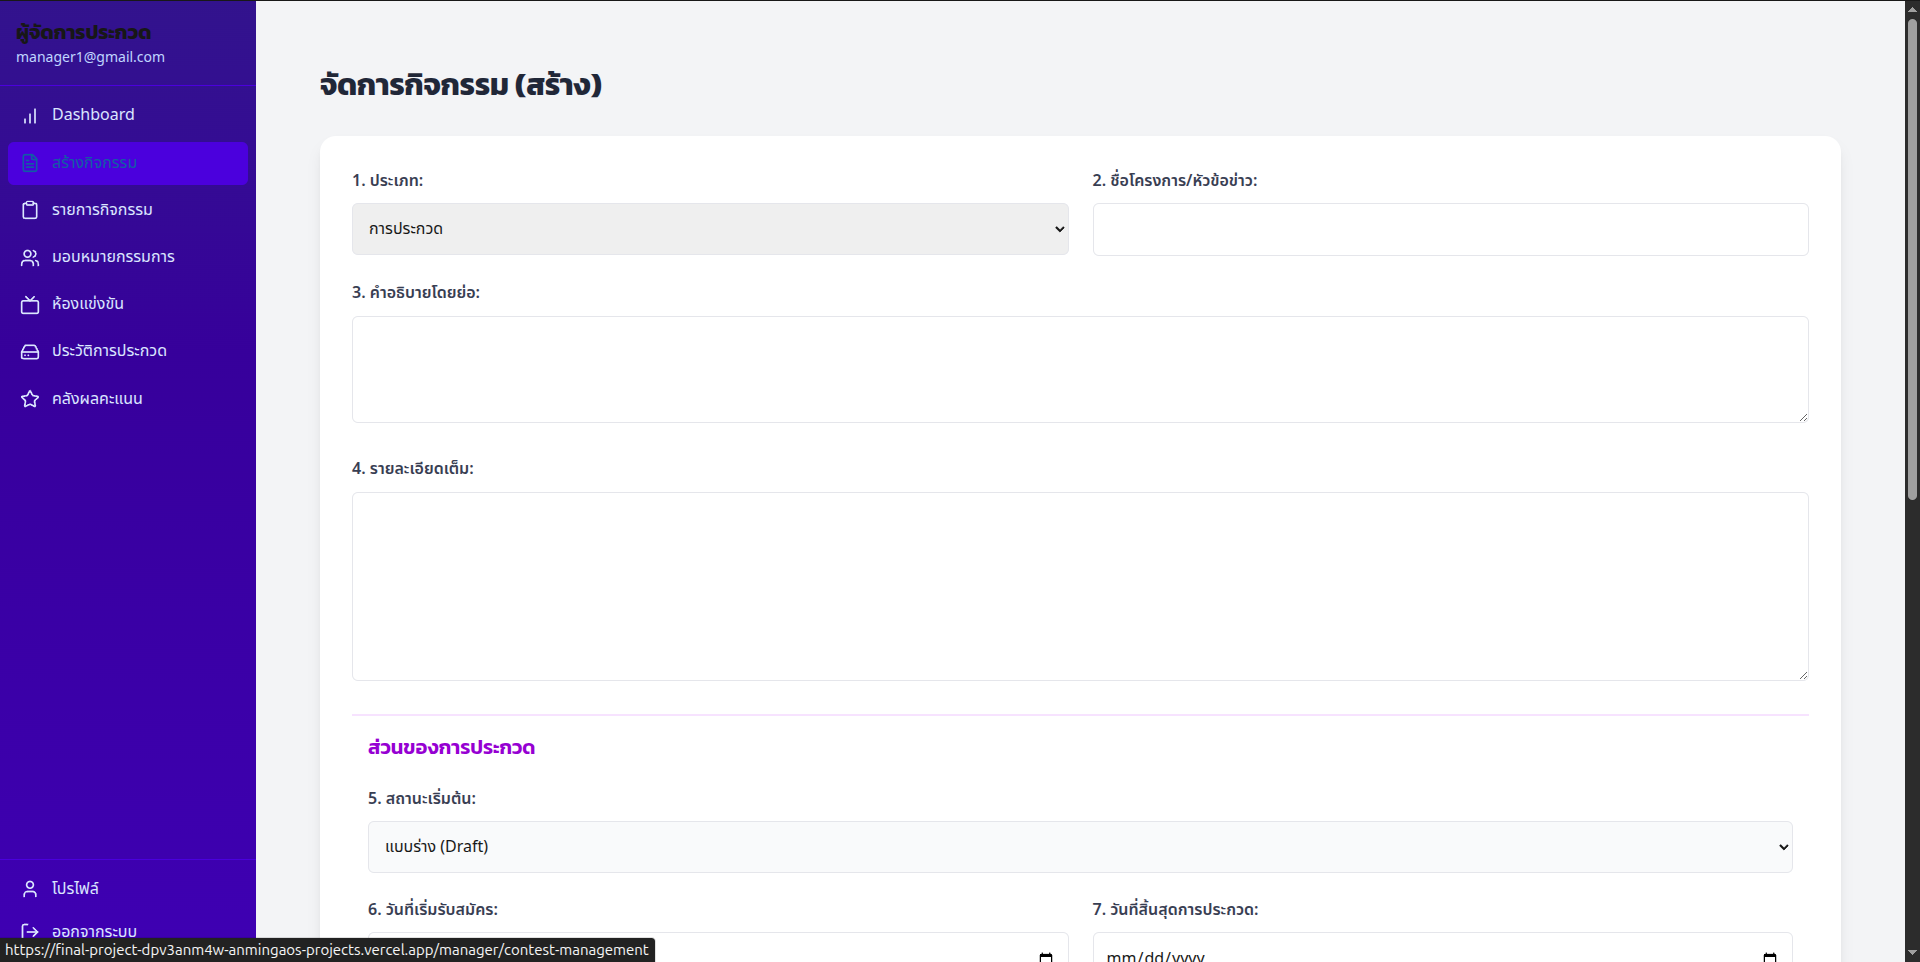
\includegraphics[width=0.8\linewidth]{MG2}
	\caption{หน้าสร้างกิจกรรมการประกวดหรือข่าวสาร}
\end{figure}

\indent หน้านี้เป็นหน้าที่ผู้จัดการใช้สำหรับ สร้าง "การประกวด" หรือ "ข่าวสาร" ใหม่ๆ เพื่อประกาศบนเว็บไซต์ โดยผู้จัดการจะต้องกรอกข้อมูลต่างๆ ให้ครบถ้วนตามแบบฟอร์ม

\newpage

\begin{figure}[h]
	\centering
	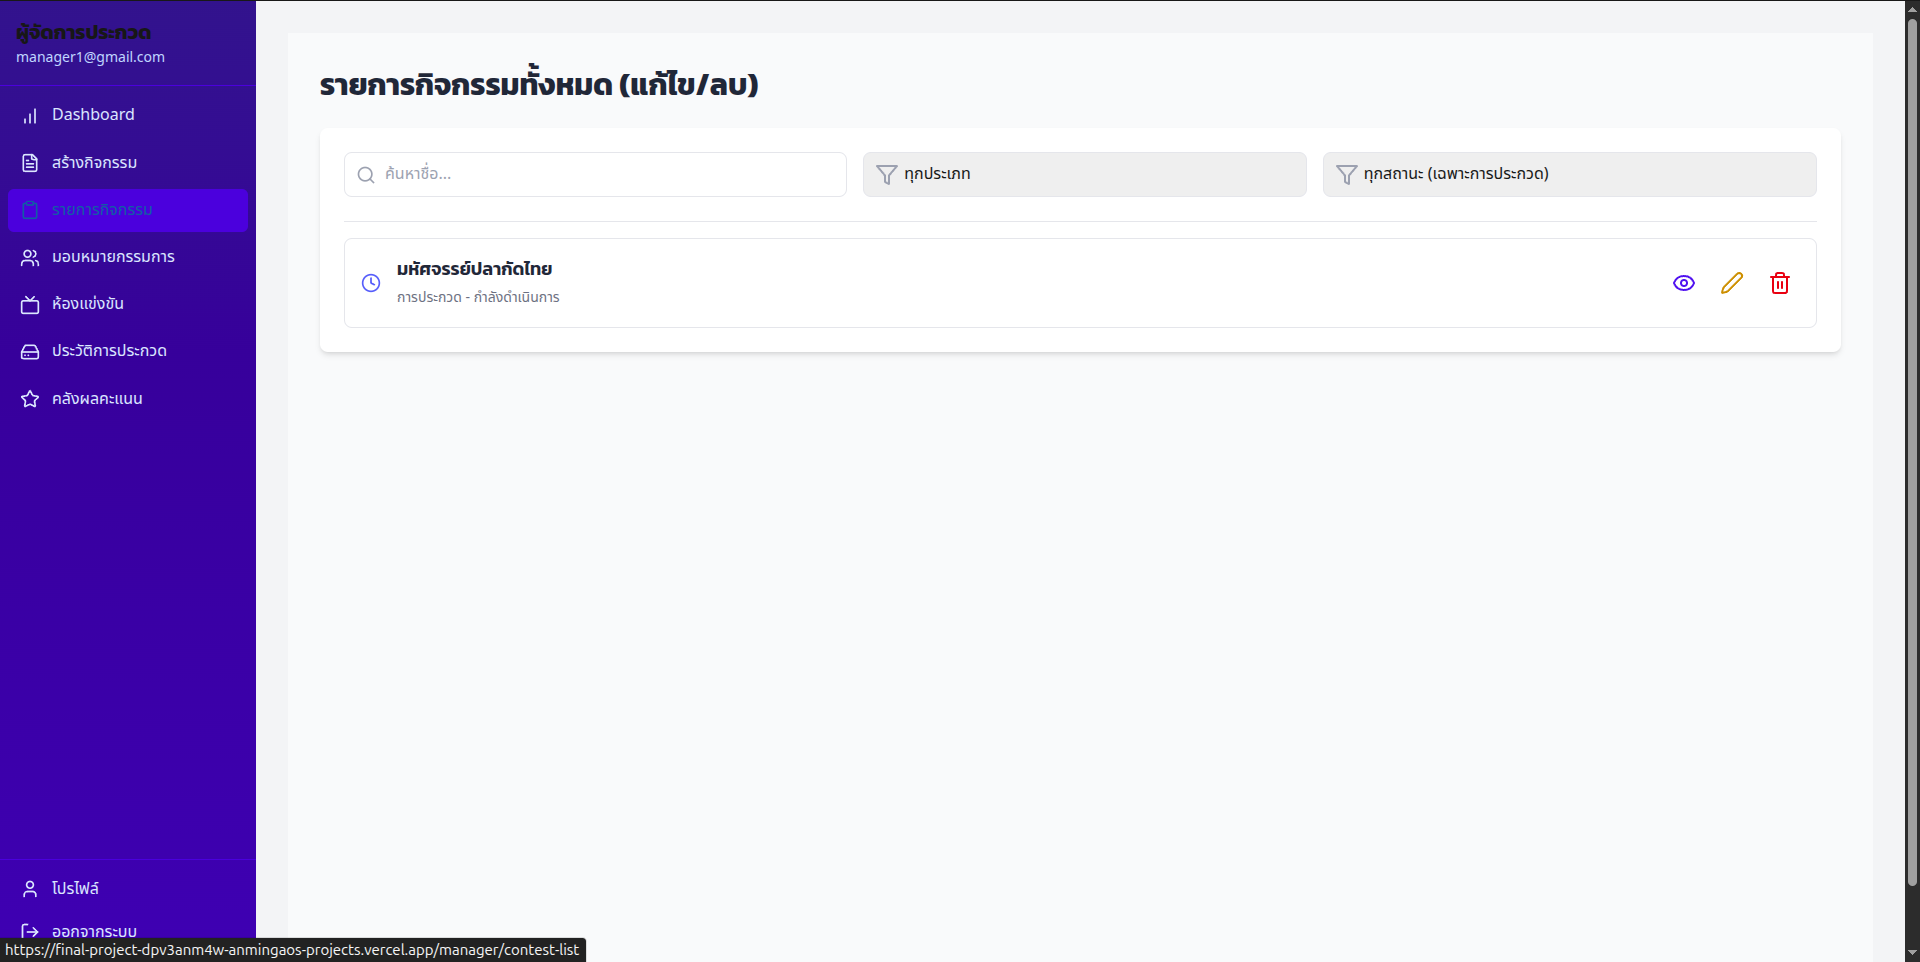
\includegraphics[width=0.8\linewidth]{MG3}
	\caption{หน้ากิจกรรมที่ได้สร้างขึ้นทั้งหมด}
\end{figure}

\indent หน้านี้เป็นเหมือนคลังเก็บกิจกรรมทั้งหมดที่ผู้จัดการเคยสร้างไว้ ไม่ว่าจะเป็น "การประกวด" หรือ "ข่าวสาร" ก็จะมารวมกันอยู่ที่นี่ทั้งหมด โดยผู้จัดการสามารถเข้ามาจัดการกิจกรรมต่างๆ ได้อย่างเต็มที่

\vspace{\baselineskip}

\begin{figure}[h]
	\centering
	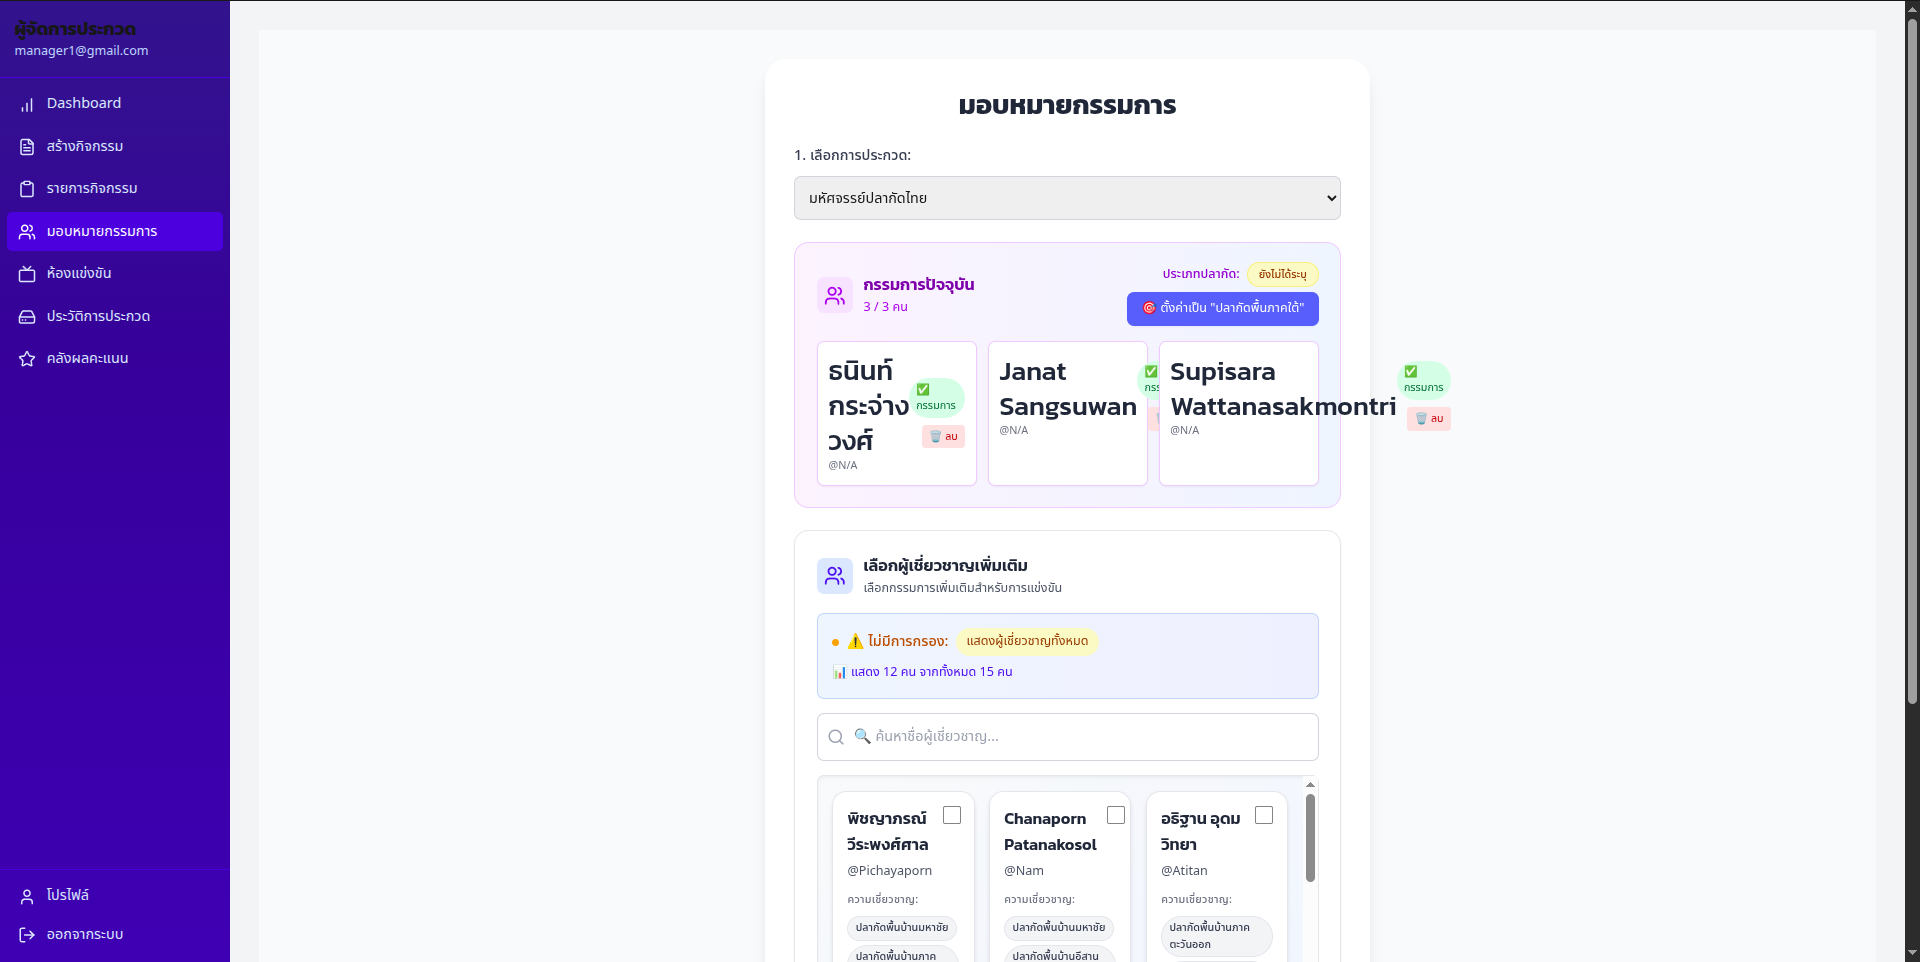
\includegraphics[width=0.8\linewidth]{MG4}
	\caption{หน้ามอบหมายกรรมการให้กิจกรรมการแข่งขัน}
\end{figure}

\indent นหน้านี้ ผู้จัดการสามารถเลือกการประกวด ผู้จัดการต้องใช้เมนู dropdown ด้านบนสุดเพื่อ เลือกการประกวด ที่ต้องการจะมอบหมายกรรมการก่อน ตรวจสอบกรรมการปัจจุบัน หลังจากเลือกการประกวดแล้ว ระบบจะแสดง "กรรมการปัจจุบัน" ที่ถูกมอบหมายให้งานนี้แล้วทำให้ผู้จัดการทราบว่าตอนนี้มีใครอยู่ในทีมตัดสินบ้าง

\newpage

\begin{figure}[h]
	\centering
	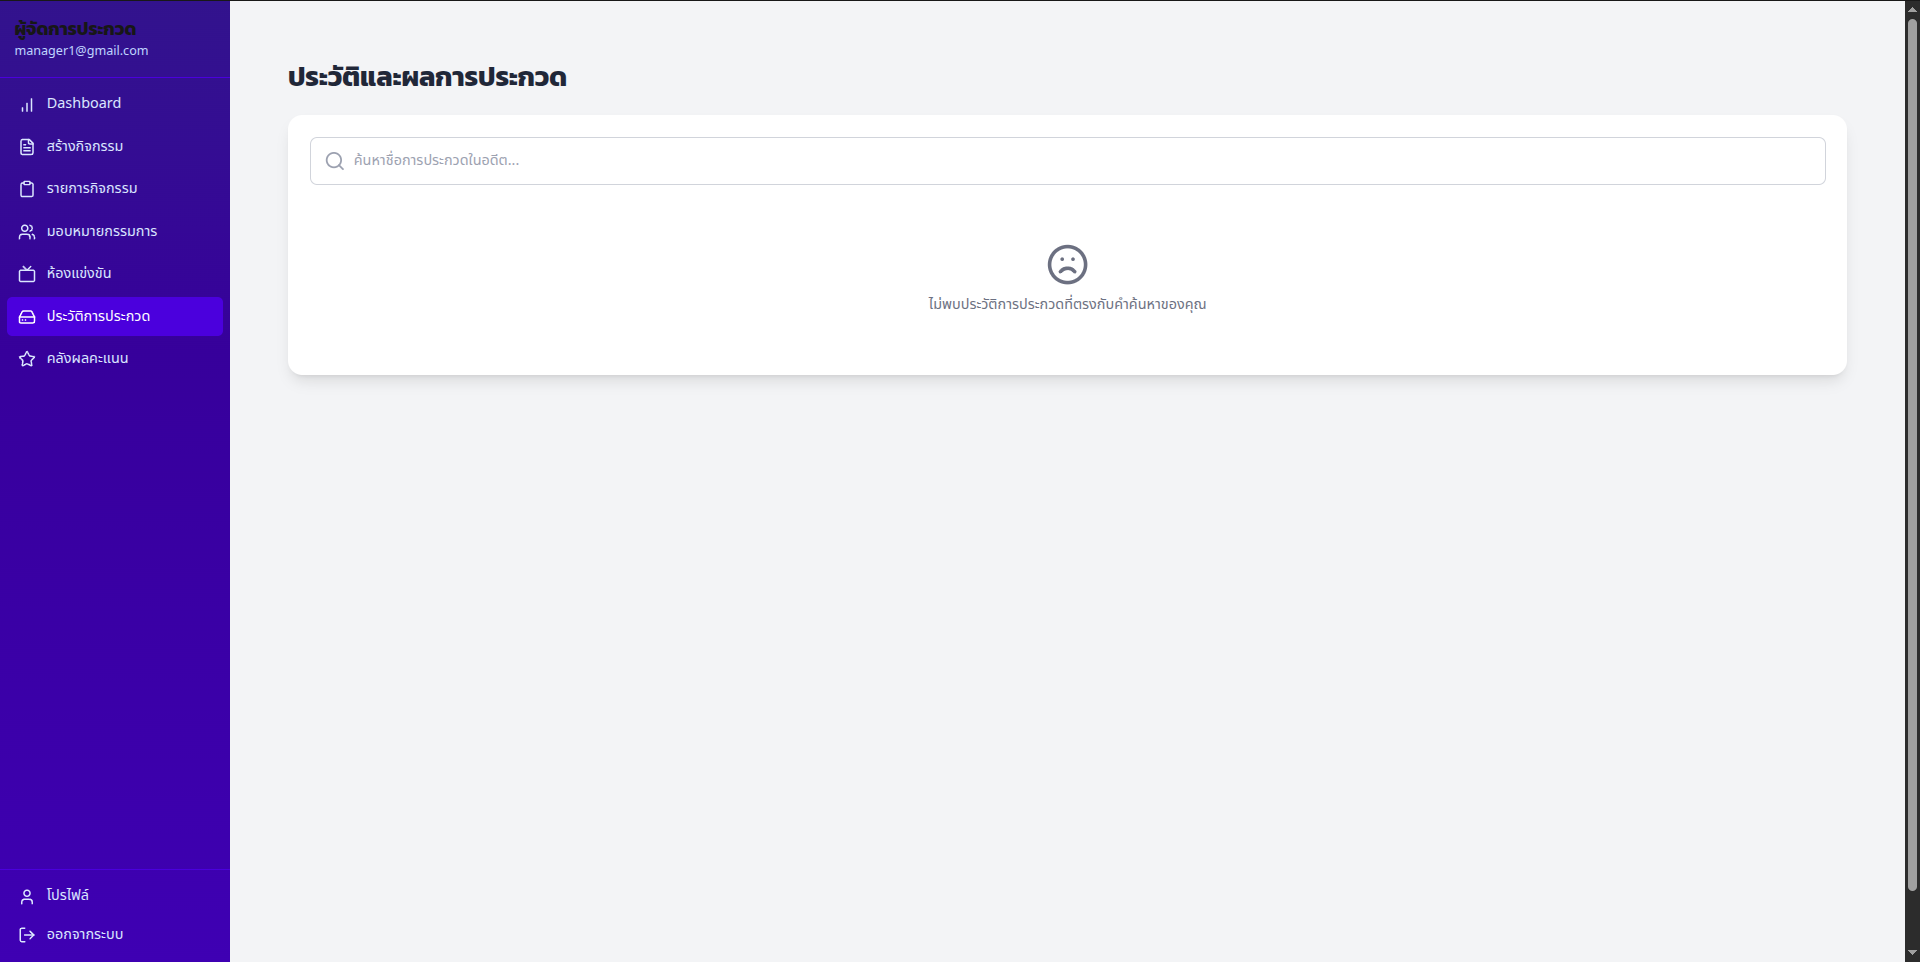
\includegraphics[width=0.8\linewidth]{MG6}
	\caption{หน้าประวติและผลการประกวด}
\end{figure}

\indent หน้านี้เปรียบเสมือนคลังเก็บข้อมูลสำหรับกิจกรรมการประกวดทั้งหมดที่ผู้จัดการเคยจัดและ เสร็จสิ้นไปแล้ว (เช่น ประกาศผลแล้ว หรือยกเลิกไป) ดูรายการประกวดที่จบไปแล้ว โดยปกติแล้ว หน้านี้จะแสดงรายการประกวดในอดีตทั้งหมดที่ผู้จัดการคนนี้เคยสร้างไว้ ทำให้สามารถย้อนกลับมาดูได้ว่าเคยจัดกิจกรรมอะไรไปบ้าง ดูผลสรุปการแข่งขัน คือส่วนที่สำคัญที่สุดครับ ในแต่ละรายการประกวดที่จบไปแล้ว จะมีปุ่ม "ดูผลสรุป" (ที่เป็นไอคอนรูปดวงตา) อยู่ข้างๆ เมื่อกดปุ่มนี้ จะมีหน้าต่าง Pop-up แสดงรายละเอียดผลการแข่งขันขึ้นมา ซึ่งจะบอกว่า ใครคือผู้ชนะ 3 อันดับแรก, ได้คะแนนรวมเท่าไหร่, และส่งปลาชื่ออะไรเข้าประกวด

\vspace{\baselineskip}

\begin{figure}[h]
	\centering
	\includegraphics[width=0.8\linewidth]{MG8}
	\caption{หน้าโปรไฟล์ผู้จัดการประกวด}
\end{figure}

\indent ในหน้านี้ ผู้จัดการสามารถทำจัดการข้อมูลส่วนตัว จัดการจะเห็นข้อมูลของตัวเอง เช่น รูปโปรไฟล์, ชื่อ, และอีเมล สามารถกดปุ่ม "แก้ไขข้อมูลส่วนตัว" เพื่อเข้าไป เปลี่ยนชื่อ-นามสกุล หรือ Username ของตัวเองได้ สามารถ คลิกที่รูปโปรไฟล์ เพื่ออัปโหลดรูปประจำตัวใหม่ได้ และยังสามารถภาพรวมและจัดการงานด่วน  ศูนย์ควบคุม จะมีสรุปตัวเลขสำคัญๆ ให้ดูอย่างรวดเร็ว เช่น ตอนนี้มี "ประกวดที่ดูแลอยู่" กี่รายการ, มี "ผู้สมัครรออนุมัติ" กี่คน, และมี "ประกวดที่เสร็จสิ้น" ไปแล้วกี่รายการ รายการที่ต้องจัดการ ส่วนนี้สำคัญมากจะแสดงรายการประกวดที่กำลังดำเนินการอยู่ (Active) ผู้จัดการสามารถดูสถานะคร่าวๆ และกดปุ่ม "จัดการ" ที่ท้ายรายการได้เลย เมื่อกดปุ่ม "จัดการ" ระบบจะพาผู้จัดการเข้าไปที่ "ห้องแข่งขัน" (Live Contest Room) ของการประกวดนั้นๆ ทันที เพื่อไปอนุมัติผู้สมัครหรือจัดการขั้นตอนต่อไป

\endgroup}{}
	
	% บทที่ 4 (ใช้หน้าใน Chapter3_28.tex เป็นหน้าบท)
	\thispagestyle{plain}
	\IfFileExists{Chapter3_28.tex}{%==================== chapter4.tex ====================

\clearpage
\thispagestyle{empty}

\begingroup
\fontsize{16pt}{19.2pt}\selectfont
\justifying
\XeTeXlinebreakskip=0pt plus 1pt minus 0.5pt
\setlength{\parindent}{1.5cm}
\setlength{\parskip}{0pt}

% ---------- หัวบท + เขียนสารบัญบทก่อนหัวข้อย่อย ----------
\phantomsection
\addcontentsline{toc}{chapter}{บทที่ 4 ผลการดำเนินงาน}
\begin{center}
	{\bfseries\fontsize{18pt}{21.6pt}\selectfont บทที่ 4}
\end{center}

\vspace{\baselineskip}

% ---------- ชื่อบท ----------
\begin{center}
	{\bfseries\fontsize{18pt}{21.6pt}\selectfont ผลการดำเนินงาน}
\end{center}

\vspace{\baselineskip}

% ---------- หัวข้อใหญ่ (ชิดซ้าย, หนา 16pt) ----------
\section*{แหล่งที่มาของข้อมูลภาพและวิธีการรวบรวม}
\addcontentsline{toc}{section}{แหล่งที่มาของข้อมูลภาพและวิธีการรวบรวม}

\indent สำหรับการได้มาซึ่งข้อมูลภาพปลากัด ผู้วิจัยใช้วิธีรับสมัครอาสาสมัครผ่านชุมชนผู้เลี้ยงปลากัดบน Facebook โดยเผยแพร่ “แบบฟอร์มเก็บข้อมูลออนไลน์” ไปยังกลุ่มที่เกี่ยวข้อง เพื่อขอความอนุเคราะห์ให้ผู้เลี้ยงปลากัดอัปโหลดภาพและระบุข้อมูลประกอบของปลาแต่ละตัว ทั้งนี้ได้แนบคำชี้แจงวัตถุประสงค์การวิจัย เงื่อนไขการใช้งานข้อมูล ก่อนการส่งแบบฟอร์ม ผู้ให้ข้อมูลต้องกดยินยอมการใช้ข้อมูลเพื่อการศึกษา/วิจัย (non-commercial) และยืนยันว่ามีสิทธิ์ในภาพดังกล่าว


% ---------- หัวข้อใหญ่ (ชิดซ้าย, หนา 16pt) ----------
\section*{ผลการทดสอบแบบจำลองปัญญาประดิษฐ์}
\addcontentsline{toc}{section}{ผลการทดสอบแบบจำลองปัญญาประดิษฐ์}

% ---------- เนื้อหา (จัดกระจายแบบไทย, ย่อหน้าแรก 1.5 ซม.) ----------
\indent ในการพัฒนาเว็บแอปพลิเคชัน “ศูนย์รวมการจัดประกวดปลากัดไทย” ผู้วิจัยได้สร้างระบบ
จัดเก็บข้อมูลการแข่งขัน ข่าวสาร และเชื่อมต่อกับแบบจำลองสำหรับการจำแนกสายพันธุ์ปลากัด ซึ่ง
โมเดลหลักที่เลือกใช้คือ ResNet50 (pre-trained บน ImageNet) พร้อมการปรับ Fine-tune
ให้เหมาะกับข้อมูลที่รวบรวมมา โดยก่อนการฝึกโมเดลมีการเตรียมข้อมูลภาพ ดังนี้


\begin{sloppypar}
	\begin{enumerate} %[start=4]  % เริ่มที่ 2 (ต่อจาก 1)
		\item \textbf{การตรวจสอบและกรองไฟล์ ภาพ:} ลือกเฉพาะไฟล์ ที่ รองรับ ได้แก่ .jpg, .jpeg, .png, .bmp,
		.webp
		\item \textbf{การทำความสะอาด (Cleaning):} เปิดภาพอย่างปลอดภัยด้วยไลบรารี PIL, แปลงเป็น RGB,ปรับขนาดด้านยาวไม่เกินที่กำหนด และบันทึกใหม่เป็น JPEG
		\item \textbf{การกำจัดภาพซ้ำ (Deduplication):} ใช้วิธี Average Hash เพื่อตรวจจับและตัดภาพที่ซ้ำหรือเกือบซ้ำ
		\item \textbf{การแบ่ง ชุด ข้อมูล (Splitting):} แบ่ง ข้อมูล เป็น Training set และ Validation set ในอัตรา 85:15 โดยสุ่มแยกต่อคลาส
	\end{enumerate}
\end{sloppypar}

\indent หลังการเตรียมข้อมูลได้ชุดข้อมูลรวมจำนวน 356 ภาพแบ่งเป็น Train 294 ภาพและ Validation 50 ภาพ

\newpage

\begin{table}[h]
	\caption{จำนวนภาพปลากัดหลังการเตรียมข้อมูล}
	{\tablefont
		\setlength{\tabcolsep}{6pt}%
		\begin{tabularx}{\linewidth}{@{}
				>{\raggedright\arraybackslash}X
				>{\centering\arraybackslash}p{2.2cm}
				>{\centering\arraybackslash}p{2.6cm}
				>{\centering\arraybackslash}p{2.2cm}
				@{}}
			\Xhline{1.5pt}
			\bfseries คลาส & \bfseries Train & \bfseries Validation & \bfseries รวม \\
			\Xhline{0.5pt}
			ปลากัดพื้นบ้านภาคอีสานหางลาย & 101 & 17 & 118 \\
			\Xhline{0.5pt}
			ปลากัดพื้นบ้านภาคใต้ & 114 & 20 & 134 \\
			\Xhline{0.5pt}
			ปลากัดพื้นบ้านมหาชัย & 79 & 13 & 92 \\
			\Xhline{0.5pt}
			รวม & 294 & 50 & 344 \\
			\Xhline{1.5pt}
	\end{tabularx}}
\end{table}

\endgroup}{}
	\IfFileExists{Chapter3_29.tex}{%==================== chapter3_29.tex ====================

\clearpage
\thispagestyle{plain}

\begingroup
\fontsize{16pt}{19.2pt}\selectfont
\justifying
\XeTeXlinebreakskip=0pt plus 1pt minus 0.5pt
\setlength{\parindent}{1.5cm}
\setlength{\parskip}{0pt}

\section*{ผลการทดสอบโมเดล ResNet50}
\addcontentsline{toc}{section}{ผลการทดสอบโมเดล ResNet50}

\indent โมเดลที่ใช้ทดลองคือ ResNet50 โดยเปลี่ยนชั้นสุดท้ายให้รองรับ 3 คลาสและทำการ
Fine-tune ด้วย Optimizer แบบ AdamW พร้อม Cosine learning rate schedule และ Early
Stopping เพื่อป้องกัน Overfitting

\begin{sloppypar}
	\begin{enumerate}
		\item ค่า \textbf{Accuracy} บนชุด Validation สูงสุด = 1.0000
		\item ค่า \textbf{Macro-F1} บนชุด Validation สูงสุด = 1.0000
	\end{enumerate}
\end{sloppypar}

\indent การหยุดการฝึกเกิดขึ้นที่ Epoch 20 จากทั้งหมด 30 Epoch ตามเกณฑ์ Early Stopping กราฟการเรียนรู้ แสดงดังรูป ซึ่งเห็นได้ว่าค่า Loss ลดลงต่อเนื่องและ Accuracy
F1-score ของ Validation set เพิ่มขึ้นจนถึง 100\% นอกจากนี้ยังได้สร้าง Confusion Matrix ดังรูป ซึ่งผลลัพธ์แสดงว่าโมเดลสามารถจำแนกได้ถูกต้องครบทุกตัวอย่างในชุด Validation

\vspace{\baselineskip}

\section*{สรุปผลการทดสอบแบบจำลอง}
\addcontentsline{toc}{section}{สรุปผลการทดสอบแบบจำลอง}
\indent โมเดลสามารถจำแนกปลากัดทั้งสามกลุ่ม (ปลากัดพื้นบ้านภาคอีสานหางลาย, ปลากัดพื้นบ้านภาคใต้, ปลากัดพื้นบ้านมหาชัย) ได้อย่างถูกต้องบน
Validation set อย่างไรก็ตาม ขนาดข้อมูลยังค่อนข้างเล็กโดยเฉพาะคลาส ปลากัดพื้นบ้านมหาชัย ที่มีจำนวน
น้อย ซึ่งอาจทำให้โมเดลมี Bias และค่า Accuracy ที่ได้สูงอาจสะท้อน Overfitting ต่อโดเมนข้อมูล
ที่ใช้ ดังนั้นควรมีการทดสอบเพิ่มเติมกับชุดข้อมูลใหม่ที่ไม่ได้อยู่ในกระบวนการฝึก เพื่อประเมินความ
สามารถทั่วไป (generalization) ของโมเดล



\begin{figure}[h]
	\centering
	\includegraphics[width=0.42\linewidth]{GF2}
	\hfill
	\includegraphics[width=0.42\linewidth]{GF1}
	\caption{กราฟ Loss ของ Train และ Validation และ Confusion Matrix ของผลการทดสอบ}
\end{figure}

\endgroup


}{}
	
	% บทที่ 5 (ใช้หน้าใน Chapter3_30.tex เป็นหน้าบท)
	\thispagestyle{plain}
	\IfFileExists{Chapter3_30.tex}{%==================== chapter3_28.tex ====================

\clearpage
\thispagestyle{empty}

\begingroup
\fontsize{16pt}{19.2pt}\selectfont
\justifying
\XeTeXlinebreakskip=0pt plus 1pt minus 0.5pt
\setlength{\parindent}{1.5cm}
\setlength{\parskip}{0pt}

% ---------- หัวบท + เขียนสารบัญบทก่อนหัวข้อย่อย ----------
\phantomsection
\addcontentsline{toc}{chapter}{บทที่ 5 บทสรุป}
\begin{center}
	{\bfseries\fontsize{18pt}{21.6pt}\selectfont บทที่ 5}
\end{center}

\vspace{\baselineskip}

% ---------- ชื่อบท ----------
\begin{center}
	{\bfseries\fontsize{18pt}{21.6pt}\selectfont บทสรุป}
\end{center}

\vspace{\baselineskip}

\indent จากการศึกษาค้นคว้า เรื่องเว็บ แอปพลิเคชัน ศูนย์ รวมการจัด ประกวดปลากัด ไทย และมี
การนำ Ai มาใช้ในการช่วยตรวจสอบประเภทปลากัด ว่าเป็นปลากัดประเภทไหน โดยมีวัตถุประสงค์
เพื่อ พัฒนาระบบเว็บ แอปพลิเคชัน ศูนย์ รวมการจัด ประกวดปลากัด ไทย โดยเราได้ ศึกษาและพัฒนา
ระบบเป็น Web Application โดยใช้ React, Visual Studio code, Supabase
การสร้างโมเดลจาก ResNet-50 เป็นการนำมาใช้ ในการสร้างต้นแบบบน Web App
Appication เนื่องจากมีการสนับสนุนร่วมกับ React,Node.js,Express โดย Web App Appication
สามารถทำการแยกประเภทปลากัด ได้ 3 ประเภทในตอนนี้สามารถทำการจำแนกได้โดยการอัปโหลดรูปภาพ 3 รูปภาพแต่เราเอารูปภาพรูปแรกเพื่อให้โมเดลดูว่าคือปลากัดประเภทไหน

\vspace{\baselineskip}

% ---------- หัวข้อใหญ่ (ชิดซ้าย, หนา 16pt) ----------
\section*{ปัญหาและอุปสรรค}
\addcontentsline{toc}{section}{ปัญหาและอุปสรรค}

\begin{sloppypar}
	\begin{enumerate}
		\item แหล่งข้อมูลในการทำ Dataset ที่เป็นรูปภาพปลากัดของแต่ละประเภท หาได้ค่อนข้างยากเพราะ
		ต้องใช้ภาพจำนวนมากต่อปลา 1 ตัว จึงต้องทำการขออนุญาตใช้ภาพจากกลุ่ม Facebook ชุมชน
		คนเลี้ยงปลากัด ที่อนุเคราะห์ให้ภาพปลากัดมาทำ Dataset
		\item เนื่องจาก Dataset ที่มีอยู่ยังไม่ครอบคลุมประเภทปลากัดพื้นบ้านทั้งหมด จึงทำให้โมเดลสามารถทำนายได้เพียง 3 คลาส ได้แก่ ปลากัดพื้นบ้านมหาชัย ปลากัดพื้นบ้านอีสานหางลาย และปลากัดพื้นบ้านภาคใต้
		\item ข้อจำกัดด้านการฝึก (Training) และการใช้งานโมเดลบนแพลตฟอร์มโฮสต์
		\begin{enumerate}
			\item ข้อจำกัดเมื่อฝึกโมเดลจริง: การฝึก ResNet50 แบบ Fine-tune ต้องใช้ทรัพยากรค่อนข้างมาก (ทั้งด้านเวลาและหน่วยประมวลผล) โดยเฉพาะเมื่อมีการทำ Augmentation และต้องจูน Hyperparameters หลายรอบ ส่งผลให้รอบการทดลอง (experiment iteration) ช้าลงและมีค่าใช้จ่ายทรัพยากรสูงเมื่อเทียบกับขนาดชุดข้อมูลที่เพิ่มขึ้น
			\item ข้อจำกัดเมื่อเผยแพร่บน Hugging Face Spaces (CPU Basic): โครงสร้างพื้นฐานที่ใช้งานแบบ \emph{CPU basic} (2 vCPU, RAM 16\,GB) ไม่มี GPU ทำให้เวลาอนุมาน (inference latency) สูงกว่าโหมดที่มี GPU โดยเฉพาะเมื่อรับภาพความละเอียดสูงหรือประมวลผลแบบหลายคำขอพร้อมกัน (concurrent requests) ส่งผลต่อประสบการณ์ผู้ใช้ในช่วงที่มีผู้ใช้งานพร้อมกัน
			\item ข้อจำกัดด้านพื้นที่และทรัพยากรหน่วยความจำ: แม้โมเดล ResNet50 จะไม่ใหญ่มากเมื่อเทียบกับสถาปัตยกรรมสมัยใหม่ แต่การรันพร้อม Pipeline ก่อน–หลังการประมวลผล (pre/post-processing) และการเก็บไฟล์เสริม (เช่น class mapping, ตัวอย่างสาธิต) อาจใช้หน่วยความจำจนกระทบเสถียรภาพของแอปเมื่อเกิดโหลดชั่วขณะ
			\item ผลกระทบจากการพักการทำงานอัตโนมัติ (Sleep after 48 hr of inactivity): เมื่อ Space เข้าสถานะพัก ระบบจะต้อง “อุ่นเครื่อง” (cold start) ใหม่ในคำขอแรกหลังตื่น ส่งผลให้การตอบสนองครั้งแรกช้าผิดปกติ และหากมีงานประมวลผลเป็นชุด (batch) หรืองานที่รออยู่ อาจสะดุดหรือหมดเวลา (timeout) ได้
			\item ความต่อเนื่องของบริการและการอัปเดต: การอัปเดตเวอร์ชันไลบรารีหรือรีสตาร์ทคอนเทนเนอร์อาจทำให้แคชโมเดลถูกล้าง ต้องดาวน์โหลด/โหลดโมเดลใหม่ (model warm-up) ทำให้ช่วงเวลาพร้อมใช้งานจริงลดลงหากไม่มีระบบแคชหรือกลไกเตรียมความพร้อม
		\end{enumerate}
		\item ผลกระทบต่อระบบเว็บแอป “ศูนย์รวมการจัดประกวดปลากัดไทย”
		\begin{enumerate}
			\item ประสบการณ์ผู้ใช้: ช่วงเวลาหน่วงสูงในคำขอแรกหลัง Space ตื่น หรือเมื่อมีผู้ใช้พร้อมกันหลายราย อาจทำให้ผู้ใช้รู้สึกว่าระบบช้า/ไม่เสถียร
			\item ข้อจำกัดด้านคุณภาพการทำนาย: เพราะชุดข้อมูลยังครอบคลุมได้เพียง 3 คลาส โมเดลจะไม่สามารถระบุประเภทอื่น ๆ ได้ ทำให้ต้องออกแบบ UX ให้รองรับกรณี “นอกคลาส” (out-of-distribution) เช่น แจ้งเตือน/เสนอให้เลือกประเภทด้วยตนเอง
		\end{enumerate}
	\end{enumerate}
\end{sloppypar}


% ---------- หัวข้อใหญ่ (ชิดซ้าย, หนา 16pt) ----------
\section*{ข้อเสนอแนะ}
\addcontentsline{toc}{section}{ข้อเสนอแนะ}

\begin{sloppypar}
	\begin{enumerate}
		\item รองรับการรับชำระเงินค่าสมัครเข้าร่วมประกวด (Payments)
		\begin{enumerate}
			\item แนวทางระบบ: แยก \emph{Payment Service} ออกเป็นโมดูล/ไมโครเซอร์วิส รับคำสั่งชำระเงินและรอ \emph{webhook} ยืนยันสถานะจากผู้ให้บริการชำระเงิน (PG) จากนั้นอัปเดตฐานข้อมูล (เช่น payments, orders) และเปลี่ยนสถานะการสมัครใน registrations เป็น paid.
			\item การเชื่อมต่อ: ใช้ Hosted Checkout/PaymentIntent ของผู้ให้บริการ (ลดภาระ PCI-DSS) พร้อมรองรับวิธีชำระเงินที่แพร่หลาย เช่น บัตร, โอน/QR, e-Wallet. ตั้งค่า \emph{webhook} ที่ปลอดภัย (ตรวจลายเซ็น/secret, IP allowlist).
			\item สคีมาฐานข้อมูล (ตัวอย่าง): \\
			payments(id, user\_id, registration\_id, amount, currency, provider, status, charge\_id, created\_at) \\
			payment\_logs(payment\_id, event\_type, payload, created\_at)
			\item ประสบการณ์ผู้ใช้: สร้างหน้าสรุปค่าธรรมเนียม, ปุ่ม ``ชำระเงิน'' และหน้า \emph{Return URL} ที่แสดงผล \emph{pending/success/failure} แบบชัดเจน พร้อมส่งหลักฐาน/ใบเสร็จ (อีเมล/ไฟล์ PDF)
			\item ความปลอดภัยและกฎระเบียบ: ไม่สัมผัสข้อมูลบัตรโดยตรง (ใช้ PG หน้าเว็บ), เปิด HTTPS บังคับ, เก็บเฉพาะ \emph{token/charge\_id}, ทำ \emph{idempotency} ในฝั่งเซิร์ฟเวอร์กันยิงซ้ำ, ล็อกธุรกรรมทุกครั้ง
		\end{enumerate}
		
		\item เปรียบเทียบปลากัดที่ชนะการประกวดกับปลากัดของผู้ใช้ (Similarity/Ranking)
		\begin{enumerate}
			\item แนวทางโมเดล: ใช้ \emph{feature extractor} เดียวกับโมเดลหลัก (ResNet50 ที่ Fine-tune แล้ว) ดึง \emph{embedding} จากชั้นก่อน FC แล้วทำ \emph{similarity search} (Cosine/Euclidean) กับฐานข้อมูลภาพผู้ชนะ
			\item เร่งความเร็วค้นหา: จัดทำดัชนีด้วย FAISS/Annoy/HNSW ให้ค้นหาใกล้เคียงแบบประมาณ (ANN) ได้เร็วเมื่อจำนวนภาพผู้ชนะเพิ่มขึ้น
			\item เมตริกและคำอธิบายผล: แสดง Top-$k$ ความใกล้เคียง พร้อมคะแนน/ระยะห่าง และ \emph{saliency/Grad-CAM} เพื่ออธิบายว่าบริเวณใดมีผลต่อความใกล้เคียง (เพิ่มความโปร่งใส)
			\item ส่วนติดต่อผู้ใช้: หน้าเปรียบเทียบแบบ \emph{side-by-side} (ภาพผู้ใช้ vs. ภาพผู้ชนะ) + ชิปคุณลักษณะเด่น (สีครีบ, ลายหาง, รูปทรงครีบ) และคำแนะนำการปรับปรุง (ถ้ามี)
			\item สคีมาฐานข้อมูล (ตัวอย่าง): \\
			winners(id, contest\_id, image\_url, class, embedding, meta) \\
			user\_images(id, user\_id, image\_url, embedding, created\_at)
			\item ถูกต้องและยุติธรรม: แจ้งผู้ใช้ว่าเป็นการ ``เปรียบเทียบเชิงลักษณะภาพ'' ไม่ใช่การตัดสินผลประกวด ลดความเข้าใจผิดเรื่องเกณฑ์กรรมการ
		\end{enumerate}
		
		\item เพิ่มจำนวนคลาสให้ครบประเภทปลากัดพื้นบ้านของไทย (Data Expansion \& Model Update)
		\begin{enumerate}
			\item กลยุทธ์ข้อมูล: ทำแคมเปญรับรูปอย่างเป็นระบบ (แบบฟอร์ม + เงื่อนไขสิทธิ์ใช้งาน), ใช้ \emph{active learning} ให้โมเดลช่วยคัดตัวอย่างที่ไม่มั่นใจเพื่อส่งให้ผู้เชี่ยวชาญช่วยติดป้ายกำกับ
			\item คุณภาพป้ายกำกับ: ใช้ผู้เชี่ยวชาญ 2 คนขึ้นไปต่อภาพ (double-blind) แล้วทำ consensus; เก็บ \emph{label provenance} และความเชื่อมั่นต่อคลาส
			\item ลดปัญหาคลาสไม่สมดุล: ใช้ \emph{class-balanced loss}, \emph{focal loss}, \emph{re-weighting}, และ \emph{augmentation} ตามลักษณะคลาส (ไม่บิดเพศ/ลักษณะจำแนก)
			\item ป้องกันข้อมูลรั่วไหล: แบ่ง \emph{train/val/test} แบบ \emph{grouped by owner/farm} ไม่ให้ภาพจากผู้ส่งเดียวกันไปอยู่หลายเซ็ต
			\item รองรับกรณีคลาสอื่น/นอกคลาส: เพิ่มคลาส ``unknown'' และตัวตรวจจับ \emph{out-of-distribution} (เช่น \emph{energy-based} หรือ \emph{Mahalanobis}) เพื่อบอกผู้ใช้อย่างปลอดภัยเมื่อโมเดลไม่มั่นใจ
			\item วงจรอัปเดตโมเดล: วาง \emph{model registry} (เวอร์ชัน, เมตริก, วันที่) และทดสอบ \emph{offline \& A/B} ก่อนสลับใช้งานจริง เพื่อลด \emph{regression}
		\end{enumerate}
		
		\item ระบบการแจ้งเตือนภายนอกสำหรับผู้เชี่ยวชาญ/ผู้จัดการประกวด (Notifications)
		\begin{enumerate}
			\item โครงสร้างเหตุการณ์: นิยามอีเวนต์หลัก (เช่น ``มีภาพรอประเมิน'', ``สมัครประกวดใหม่'', ``ต้องอนุมัติ/ปฏิเสธ'', ``ชำระเงินสำเร็จ''). ใช้ \emph{event bus} กลาง (เช่น database trigger $\rightarrow$ queue) แล้วค่อยกระจายไปช่องทางปลายทาง
			\item ช่องทางแจ้งเตือน: 
			\begin{itemize}
				\item \emph{Email}: ส่งสรุปรายวัน+เรียลไทม์เมื่อสำคัญ
				\item \emph{Web Push}: ผ่าน FCM สำหรับผู้ใช้ที่ยินยอม
				\item \emph{Chat Ops}: LINE Notify/Telegram Bot สำหรับทีมงาน (ห้องเฉพาะกิจ)
			\end{itemize}
			\item การบังคับใช้และกำกับสิทธิ์: ตั้งค่าการสมัครรับแจ้งเตือนรายบทบาท (ผู้เชี่ยวชาญ/ผู้จัด), ฟิลเตอร์ชนิดอีเวนต์, และช่วงเวลาเงียบ (Do-Not-Disturb)
			\item สคีมาฐานข้อมูล (ตัวอย่าง): \\
			notifications(id, user\_id, type, payload, status, channel, created\_at) \\
			subscriptions(user\_id, channel, event\_type, enabled, quiet\_hours)
			\item ความเชื่อถือได้: ใช้คิวงานพร้อม \emph{retry/backoff}, ทำ \emph{dead-letter queue}, และบันทึก \emph{delivery logs}. ทุกข้อความมี \emph{idempotency key} ป้องกันส่งซ้ำ
			\item อินทิเกรตกับระบบเดิม: หากใช้ Supabase/PG ให้ใช้ trigger $\rightarrow$ \emph{Edge Function} ยิงแจ้งเตือนเมื่อแถวในตาราง submissions, assignments, registrations, payments เปลี่ยนสถานะ
		\end{enumerate}
	\end{enumerate}
	
	\vspace{0.5em}
	\noindent Roadmap แนะนำ (ลำดับทำงาน): 
	\begin{enumerate}
		\item เปิดรับชำระเงิน (เพื่อลดภาระงานมือและสร้างรายได้ทันที)
		\item ระบบแจ้งเตือนภายนอก (ลดงานค้าง ช่วยการประสานงาน)
		\item เปรียบเทียบผู้ชนะ vs. ภาพผู้ใช้ (เพิ่มคุณค่า/แรงจูงใจ)
		\item ขยายคลาสให้ครบ (ลงทุนระยะกลาง-ยาว ยกระดับคุณภาพโมเดล)
	\end{enumerate}
\end{sloppypar}
}{}
	
	% ===== ส่วนท้าย =====
	% บรรณานุกรม
	\chapter*{บรรณานุกรม}
	\addcontentsline{toc}{chapter}{บรรณานุกรม}
	\thispagestyle{plain}
	\nocite{*}
	\printbibliography[heading=thai-bib]
	
	% ภาคผนวก
	\chapter*{ภาคผนวก}
	\addcontentsline{toc}{chapter}{ภาคผนวก}
	\thispagestyle{plain}
	\IfFileExists{Appendix.tex}{%==================== Appendix.tex ====================

\clearpage
\thispagestyle{empty}

\begingroup
% เนื้อหาภาคผนวก: 16pt baseline ~19.2pt ตามสเปกเล่ม
\fontsize{16pt}{19.2pt}\selectfont
\justifying
\XeTeXlinebreakskip=0pt plus 1pt minus 0.5pt
\setlength{\parindent}{1.5cm}
\setlength{\parskip}{0pt}

% ---------- หัวข้อใหญ่ (ชิดซ้าย, หนา 16pt) ----------
\noindent{\bfseries\fontsize{16pt}{19.2pt}\selectfont ภาคผนวก ก}\par
\noindent{\bfseries\fontsize{16pt}{19.2pt}\selectfont ผลการทดสอบโมเดล}\par

\indent ในการพัฒนาเว็บแอปพลิเคชัน “ศูนย์รวมการจัดประกวดปลากัดไทย” ผู้วิจัยได้สร้างระบบ
จัดเก็บข้อมูลการแข่งขัน ข่าวสาร และเชื่อมต่อกับแบบจำลองสำหรับการจำแนกสายพันธุ์ปลากัด ซึ่ง
โมเดลหลักที่เลือกใช้คือ ResNet50 (pre-trained บน ImageNet) พร้อมการปรับ Fine-tune
ให้เหมาะกับข้อมูลที่รวบรวมมา โดยก่อนการฝึกโมเดลมีการเตรียมข้อมูลภาพ ดังนี้

\begin{sloppypar}
	\begin{enumerate} %[start=4]  % เริ่มที่ 2 (ต่อจาก 1)
		\item \textbf{การตรวจสอบและกรองไฟล์ ภาพ:} ลือกเฉพาะไฟล์ ที่ รองรับ ได้แก่ .jpg, .jpeg, .png, .bmp,
		.webp
		\item \textbf{การทำความสะอาด (Cleaning):} เปิดภาพอย่างปลอดภัยด้วยไลบรารี PIL, แปลงเป็น RGB,ปรับขนาดด้านยาวไม่เกินที่กำหนด และบันทึกใหม่เป็น JPEG
		\item \textbf{การกำจัดภาพซ้ำ (Deduplication):} ใช้วิธี Average Hash เพื่อตรวจจับและตัดภาพที่ซ้ำหรือเกือบซ้ำ
		\item \textbf{การแบ่ง ชุด ข้อมูล (Splitting):} แบ่ง ข้อมูล เป็น Training set และ Validation set ในอัตรา 85:15 โดยสุ่มแยกต่อคลาส
	\end{enumerate}
\end{sloppypar}

\indent หลังการเตรียมข้อมูลได้ชุดข้อมูลรวมจำนวน 356 ภาพแบ่งเป็น Train 294 ภาพและ Validation 50 ภาพ

\begin{table}[h]
	\caption{จำนวนภาพปลากัดหลังการเตรียมข้อมูล}
	{\tablefont
		\setlength{\tabcolsep}{6pt}%
		\begin{tabularx}{\linewidth}{@{}
				>{\raggedright\arraybackslash}X
				>{\centering\arraybackslash}p{2.2cm}
				>{\centering\arraybackslash}p{2.6cm}
				>{\centering\arraybackslash}p{2.2cm}
				@{}}
			\Xhline{1.5pt}
			\bfseries คลาส & \bfseries Train & \bfseries Validation & \bfseries รวม \\
			\Xhline{0.5pt}
			ปลากัดพื้นบ้านภาคอีสานหางลาย & 101 & 17 & 118 \\
			\Xhline{0.5pt}
			ปลากัดพื้นบ้านภาคใต้ & 114 & 20 & 134 \\
			\Xhline{0.5pt}
			ปลากัดพื้นบ้านมหาชัย & 79 & 13 & 92 \\
			\Xhline{0.5pt}
			รวม & 294 & 50 & 344 \\
			\Xhline{1.5pt}
	\end{tabularx}}
\end{table}

\clearpage

}{}
	
	% ประวัติผู้วิจัย
	\chapter*{ประวัติผู้วิจัย}
	\addcontentsline{toc}{chapter}{ประวัติผู้วิจัย}
	\thispagestyle{plain}
	\IfFileExists{Biography.tex}{\clearpage
\thispagestyle{empty}


% ทั้งหน้า 13pt (baseline ~15.6pt)
\fontsize{16pt}{24pt}\selectfont

% จัดเต็มบรรทัดแบบไทย + ย่อหน้า 1.5 ซม.
\justifying
\XeTeXlinebreakskip=0pt plus 1pt minus 0.5pt
\setlength{\parindent}{1.5cm}
\setlength{\parskip}{0pt}

\phantomsection
\addcontentsline{toc}{chapter}{ประวัติผู้วิจัย}
\begin{center}
	{\bfseries\fontsize{16pt}{19.2pt}\selectfont ประวัติผู้วิจัย}
\end{center}
\vspace{\baselineskip}



% ---------- จัดบรรทัด "ป้ายกำกับ : ค่า" ให้ตรงคอลัมน์ ----------

\settowidth{\FieldLabelWidth}{\bfseries ประเภทสารนิพนธ์ :}

% ป้ายกำกับบรรทัดแรก "ตัวหนา 13pt" + ค่า "13pt ธรรมดา" อยู่บรรทัดเดียวกัน
% ถ้าค่ายาวจะตัดบรรทัดภายในคอลัมน์ขวาและชิดซ้ายใต้คอลัมน์ค่าเดิมเสมอ
\newcommand{\Field}[2]{%
	\noindent
	\makebox[\FieldLabelWidth][l]{\bfseries #1 :}%
	\hspace{\FieldSep}%
	\parbox[t]{\dimexpr\linewidth-\FieldLabelWidth-\FieldSep\relax}{#2}%
	\par
}

% ---------- บล็อกข้อมูลหัวเรื่อง ----------
\Field{ชื่อ-สกุล}{เอกสิทธิ์ อัศวดารา}
\Field{วัน เดือน ปี เกิด}{17 กรกฎาคม 2546}
\Field{สถานที่เกิด}{จังหวัดพิษณุโลก}
\Field{วุฒิการศึกษา}{-}
\Field{ที่อยู่ปัจจุบัน}{66/4 หมู่ที่ 4 ตำบลชาติตระการ อพเภาชาติตระการ จังหวัดพิษณุโลก 65170}

% เว้น 1 บรรทัด
\vspace{\baselineskip}}{}
	
\end{document}
